%%%%%%%%%%%%%%%%%%%%%%%%%%%%%%%%%%%%%%%%%
% Masters/Doctoral Thesis 
% LaTeX Template
% Version 2.5 (27/8/17)
%
% This template was downloaded from:
% http://www.LaTeXTemplates.com
%
% Version 2.x major modifications by:
% Vel (vel@latextemplates.com)
%
% This template is based on a template by:
% Steve Gunn (http://users.ecs.soton.ac.uk/srg/softwaretools/document/templates/)
% Sunil Patel (http://www.sunilpatel.co.uk/thesis-template/)
%
% Template license:
% CC BY-NC-SA 3.0 (http://creativecommons.org/licenses/by-nc-sa/3.0/)
%
%%%%%%%%%%%%%%%%%%%%%%%%%%%%%%%%%%%%%%%%%

%----------------------------------------------------------------------------------------
%	PACKAGES AND OTHER DOCUMENT CONFIGURATIONS
%----------------------------------------------------------------------------------------

\documentclass[
11pt, % The default document font size, options: 10pt, 11pt, 12pt
%oneside, % Two side (alternating margins) for binding by default, uncomment to switch to one side
english, % ngerman for German
onehalfspacing %onehalfspacing %singlespacing, % Single line spacing, alternatives: onehalfspacing or doublespacing
%draft, % Uncomment to enable draft mode (no pictures, no links, overfull hboxes indicated)
%nolistspacing, % If the document is onehalfspacing or doublespacing, uncomment this to set spacing in lists to single
%liststotoc, % Uncomment to add the list of figures/tables/etc to the table of contents
%toctotoc, % Uncomment to add the main table of contents to the table of contents
parskip, % Uncomment to add space between paragraphs
%nohyperref, % Uncomment to not load the hyperref package
headsepline, % Uncomment to get a line under the header
%chapterinoneline, % Uncomment to place the chapter title next to the number on one line
%consistentlayout, % Uncomment to change the layout of the declaration, abstract and acknowledgements pages to match the default layout
]{MastersDoctoralThesis} % The class file specifying the document structure

\usepackage{amsmath}
\usepackage{algpseudocode}
\usepackage{algorithm}


\algnewcommand\algorithmicforeach{\textbf{for each}}
\algdef{S}[FOR]{ForEach}[1]{\algorithmicforeach\ #1\ \algorithmicdo}

\makeatletter
\def\BState{\State\hskip-\ALG@thistlm}
\makeatother

\setlength{\parskip}{1.5em}


\usepackage[utf8]{inputenc} % Required for inputting international characters
\usepackage[T1]{fontenc} % Output font encoding for international characters

\usepackage{mathpazo} % Use the Palatino font by default
\usepackage{siunitx}
\usepackage[backend=bibtex,style=authoryear,natbib=true]{biblatex} % Use the bibtex backend with the authoryear citation style (which resembles APA)

\usepackage{titlesec}

\setcounter{secnumdepth}{5}

\titleformat{\paragraph}
{\normalfont\normalsize\bfseries}{\theparagraph}{1em}{}
\titlespacing*{\paragraph}
{0pt}{3.25ex plus 1ex minus .2ex}{1.5ex plus .2ex}

\titleformat{\subparagraph}
{\normalfont\normalsize\bfseries}{\thesubparagraph}{1em}{}
\titlespacing*{\subparagraph}
{0pt}{3.25ex plus 1ex minus .2ex}{1.5ex plus .2ex}

\addbibresource{example.bib} % The filename of the bibliography

\usepackage[autostyle=true]{csquotes} % Required to generate language-dependent quotes in the bibliography

%----------------------------------------------------------------------------------------
%	MARGIN SETTINGS
%----------------------------------------------------------------------------------------

\geometry{
	paper=a4paper, % Change to letterpaper for US letter
	inner=2.5cm, % Inner margin
	outer=3.8cm, % Outer margin
	bindingoffset=.5cm, % Binding offset
	top=1.5cm, % Top margin
	bottom=1.5cm, % Bottom margin
	%showframe, % Uncomment to show how the type block is set on the page
}

%----------------------------------------------------------------------------------------
%	THESIS INFORMATION
%----------------------------------------------------------------------------------------

\thesistitle{Interactive visualization for volumetric datasets } % Your thesis title, this is used in the title and abstract, print it elsewhere with \ttitle
\supervisor{Christophe \textsc{Hurter}} % Your supervisor's name, this is used in the title page, print it elsewhere with \supname
\examiner{} % Your examiner's name, this is not currently used anywhere in the template, print it elsewhere with \examname
\degree{Doctor of Philosophy} % Your degree name, this is used in the title page and abstract, print it elsewhere with \degreename
\author{Michael \textsc{Traor\'e}} % Your name, this is used in the title page and abstract, print it elsewhere with \authorname
\addresses{} % Your address, this is not currently used anywhere in the template, print it elsewhere with \addressname

\subject{Computer Science} % Your subject area, this is not currently used anywhere in the template, print it elsewhere with \subjectname
\keywords{} % Keywords for your thesis, this is not currently used anywhere in the template, print it elsewhere with \keywordnames
\university{\href{https://www.isae-supaero.fr/en/}{Institut supérieur de l'aéronautique et de l'espace (ISAE-SUPAERO)}} % Your university's name and URL, this is used in the title page and abstract, print it elsewhere with \univname
\department{\href{http://www.enac.fr}{\'Ecole Nationale de l'Aviation Civile (ENAC)}} % Your department's name and URL, this is used in the title page and abstract, print it elsewhere with \deptname
\group{\href{http://devi.recherche.enac.fr}{Data Economics and Interactive Visualization (DEVI)}} % Your research group's name and URL, this is used in the title page, print it elsewhere with \groupname
\faculty{\href{http://faculty.university.com}{Faculty Name}} % Your faculty's name and URL, this is used in the title page and abstract, print it elsewhere with \facname

\AtBeginDocument{
\hypersetup{pdftitle=\ttitle} % Set the PDF's title to your title
\hypersetup{pdfauthor=\authorname} % Set the PDF's author to your name
\hypersetup{pdfkeywords=\keywordnames} % Set the PDF's keywords to your keywords
}


\usepackage{amssymb}
\usepackage{array,longtable}

\newcounter{mquestion}
\newcounter{row}

\makeatletter
\newtoks\@tabtoks
\newcommand\addtabtoks[1]{\@tabtoks\expandafter{\the\@tabtoks#1}}
\newcommand*\resettabtoks{\@tabtoks{}}
\newcommand*\printtabtoks{\the\@tabtoks}
\makeatother

\newcommand\CheckTable[1]{%
  \setcounter{mquestion}{0}
  \setcounter{row}{0}
  \resettabtoks
  \loop\ifnum\therow<#1\relax
    \stepcounter{row}
    \addtabtoks{& $\square$ & $\square$ & $\square$ & $\square$ & $\square$ \\}%
  \repeat
  \begin{longtable}{>{\stepcounter{mquestion}}l*{5}{c}}
    \multicolumn{1}{c}{} & Bad & Not Bad & Neutral & OK & Good \\
    \printtabtoks
  \end{longtable}%
}


\newcommand\CheckTablelevel[1]{%
  \setcounter{mquestion}{0}
  \setcounter{row}{0}
  \resettabtoks
  \loop\ifnum\therow<#1\relax
    \stepcounter{row}
    \addtabtoks{& $\square$ & $\square$ & $\square$ & $\square$ & $\square$ \\}%
  \repeat
  \begin{longtable}{>{\stepcounter{mquestion}}l*{5}{c}}
    \multicolumn{1}{c}{} & Novice &  Adv. Beginner &  Competent & Proficient  & Expert \\
    \printtabtoks
  \end{longtable}%
}

\newcommand\CheckTableDifficulty[1]{%
  \setcounter{mquestion}{0}
  \setcounter{row}{0}
  \resettabtoks
  \loop\ifnum\therow<#1\relax
    \stepcounter{row}
    \addtabtoks{& $\square$ & $\square$ & $\square$ & $\square$ & $\square$ \\}%
  \repeat
  \begin{longtable}{>{\stepcounter{mquestion}}l*{5}{c}}
    \multicolumn{1}{c}{} & Easy & Quite Easy & Neutral & Quite Hard & Hard \\
    \printtabtoks
  \end{longtable}%
}


\usepackage{xpatch}% http://ctan.org/pkg/etoolbox
\xpatchcmd{\answerline}% <cmd>
  {\par\nobreak\vskip\answerskip}% <search>
  {}% <replace>
  {}{}% <success><failure>

\newcommand{\leftanswerline}[1][]%
{\ifthenelse{\equal{#1}{}}%
{\par\hspace{-1.3em}\begin{minipage}{1em}\answerline\end{minipage}}%
{\par\hspace{-1.3em}\begin{minipage}{1em}\answerline[#1]\end{minipage}}%
}

\begin{document}

\frontmatter % Use roman page numbering style (i, ii, iii, iv...) for the pre-content pages

\pagestyle{plain} % Default to the plain heading style until the thesis style is called for the body content

%----------------------------------------------------------------------------------------
%	TITLE PAGE
%----------------------------------------------------------------------------------------

\begin{titlepage}
\begin{center}

\vspace*{.06\textheight}
{\scshape\LARGE \univname\par}\vspace{1.5cm} % University name
\textsc{\Large Doctoral Thesis}\\[0.5cm] % Thesis type

\HRule \\[0.4cm] % Horizontal line
{\huge \bfseries \ttitle\par}\vspace{0.4cm} % Thesis title
\HRule \\[1.5cm] % Horizontal line
 
\begin{minipage}[t]{0.4\textwidth}
\begin{flushleft} \large
\emph{Author:}\\
\href{https://www.linkedin.com/in/michael-traor%C3%A9-1a620596/}{\authorname} % Author name - remove the \href bracket to remove the link
\end{flushleft}
\end{minipage}
\begin{minipage}[t]{0.4\textwidth}
\begin{flushright} \large
\emph{Supervisor:} \\
\href{http://recherche.enac.fr/~hurter/}{\supname} % Supervisor name - remove the \href bracket to remove the link  
\end{flushright}
\end{minipage}\\[3cm]
 
\vfill

\large \textit{A thesis submitted in fulfillment of the requirements\\ for the degree of \degreename}\\[0.3cm] % University requirement text
\textit{in the}\\[0.4cm]
\groupname\\\deptname\\[2cm] % Research group name and department name
 
\vfill

{\large \today}\\[4cm] % Date
%\includegraphics{Logo} % University/department logo - uncomment to place it
 
\vfill
\end{center}
\end{titlepage}

%----------------------------------------------------------------------------------------
%	DECLARATION PAGE
%----------------------------------------------------------------------------------------

\begin{declaration}
\addchaptertocentry{\authorshipname} % Add the declaration to the table of contents
\noindent I, \authorname, declare that this thesis titled, \enquote{\ttitle} and the work presented in it are my own. I confirm that:

\begin{itemize} 
\item This work was done wholly or mainly while in candidature for a research degree at this University.
\item Where any part of this thesis has previously been submitted for a degree or any other qualification at this University or any other institution, this has been clearly stated.
\item Where I have consulted the published work of others, this is always clearly attributed.
\item Where I have quoted from the work of others, the source is always given. With the exception of such quotations, this thesis is entirely my own work.
\item I have acknowledged all main sources of help.
\item Where the thesis is based on work done by myself jointly with others, I have made clear exactly what was done by others and what I have contributed myself.\\
\end{itemize}
 
\noindent Signed:\\
\rule[0.5em]{25em}{0.5pt} % This prints a line for the signature
 
\noindent Date:\\
\rule[0.5em]{25em}{0.5pt} % This prints a line to write the date
\end{declaration}

\cleardoublepage


%----------------------------------------------------------------------------------------
%	QUOTATION PAGE
%----------------------------------------------------------------------------------------

\vspace*{0.2\textheight}

\noindent\enquote{\itshape Thanks to my solid academic training, today I can write hundreds of words on virtually any topic without possessing a shred of information, which is how I got a good job in journalism.}\bigbreak

\hfill Dave Barry

%----------------------------------------------------------------------------------------
%	ABSTRACT PAGE
%----------------------------------------------------------------------------------------

\begin{abstract}
\addchaptertocentry{\abstractname} % Add the abstract to the table of contents

abstract here
\end{abstract}

%----------------------------------------------------------------------------------------
%	ACKNOWLEDGEMENTS
%----------------------------------------------------------------------------------------

\begin{acknowledgements}
\addchaptertocentry{\acknowledgementname} % Add the acknowledgements to the table of contents
The acknowledgments and the people to thank go here, don't forget to include your project advisor\ldots
\end{acknowledgements}

%---------------------------------------------------------------------------------------
%  Publications
%----------------------------------------------------------------------------------------
\begin{publications}
\addchaptertocentry{\publicationname} % Add the acknowledgements to the table of contents
Here are listed all of my publications during this thesis: \ldots
\begin{enumerate}

\item \textbf{ Journal }: Michael Traor\'e and Christophe Hurter, "Interactive Exploration of 3D Scanned Baggage", in IEEE Computer Graphics and Applications, vol. 37, no. 1, pp. 27-33, Jan.-Feb. 2017.
\item \textbf{ Conference + Journal} : Michael Traor\'e , Christophe Hurter, and Alexandru Telea, "Interactive Obstruction-free Lensing for Volumetric Data Visualization", 2018 IEEE Scientific Visualization Conference (SciVis  TVCG SI), Berlin, Germany
\item \textbf{ Patent } : HURTER, Christophe et SOMPAGNIMDI, Michael TRAORÉ. "Object definition in virtual 3D environment". U.S. Patent Application No 15/466,991, 28 sept. 2017.
\item \textbf{ Patent } : HURTER, Christophe et SOMPAGNIMDI, Michael TRAORÉ. "Boolean object management in 3D display". U.S. Patent Application No 15/466,497, 28 sept. 2017.
\item \textbf{ Patent } : HURTER, Christophe et SOMPAGNIMDI, Michael TRAORÉ. "Selective display in a computer generated environment". U.S. Patent Application No 15/485,828, 19 oct. 2017.

\end{enumerate}

\end{publications}


%----------------------------------------------------------------------------------------
%	LIST OF CONTENTS/FIGURES/TABLES PAGES
%----------------------------------------------------------------------------------------

\tableofcontents % Prints the main table of contents

\listoffigures % Prints the list of figures

\listoftables % Prints the list of tables

%----------------------------------------------------------------------------------------
%	ABBREVIATIONS
%----------------------------------------------------------------------------------------

\begin{abbreviations}{ll} % Include a list of abbreviations (a table of two columns)

\textbf{DVR} & \textbf{D}irect \textbf{V}olume \textbf{R}endering\\
\textbf{AR} & \textbf{A}ugmented \textbf{R}eality \\
\textbf{MR} & \textbf{M}ixed \textbf{R}eality \\
\textbf{VR} & \textbf{V}irtual \textbf{R}eality \\
\textbf{TF} & \textbf{T}ransfer \textbf{F}unction \\

\end{abbreviations}





%----------------------------------------------------------------------------------------
%	PHYSICAL CONSTANTS/OTHER DEFINITIONS
%----------------------------------------------------------------------------------------

%\begin{constants}{lr@{${}={}$}l} % The list of physical constants is a three column table

% The \SI{}{} command is provided by the siunitx package, see its documentation for instructions on how to use it

%Speed of Light & $c_{0}$ & \SI{2.99792458e8}{\meter\per\second} (exact)\\
%%Constant Name & $Symbol$ & $Constant Value$ with units\\

%\end{constants}

%----------------------------------------------------------------------------------------
%	SYMBOLS
%----------------------------------------------------------------------------------------
%\begin{comment}
%\begin{symbols}{lll} % Include a list of Symbols (a three column table)

%$a$ & distance & \si{\meter} \\
%$P$ & power & \si{\watt} (\si{\joule\per\second}) \\
%%Symbol & Name & Unit \\

%\addlinespace % Gap to separate the Roman symbols from the Greek

%$\omega$ & angular frequency & \si{\radian} \\

%\end{symbols}

%----------------------------------------------------------------------------------------
%	DEDICATION
%----------------------------------------------------------------------------------------

\dedicatory{For/Dedicated to/To my\ldots} 

%----------------------------------------------------------------------------------------
%	THESIS CONTENT - CHAPTERS
%----------------------------------------------------------------------------------------

\mainmatter % Begin numeric (1,2,3...) page numbering

\pagestyle{thesis} % Return the page headers back to the "thesis" style

% Include the chapters of the thesis as separate files from the Chapters folder
% Uncomment the lines as you write the chapters

% Chapter 1

\chapter{Introduction} % Main chapter title

\label{Introduction} % For referencing the chapter elsewhere, use \ref{Chapter1} 

%----------------------------------------------------------------------------------------

% Define some commands to keep the formatting separated from the content 
\newcommand{\keyword}[1]{\textbf{#1}}
\newcommand{\tabhead}[1]{\textbf{#1}}
\newcommand{\code}[1]{\texttt{#1}}
\newcommand{\file}[1]{\texttt{\bfseries#1}}
\newcommand{\option}[1]{\texttt{\itshape#1}}

%----------------------------------------------------------------------------------------

\section{Synthèse}

\subsection{Contexte}
Les jeux de donnes volumétriques sont présents dans de nombreux domaines tels que l'imagerie médicale, la physique, les sciences naturelles, la sécurité, l'ingénierie, etc... Ils sont composés de voxels qui représentent la forme de ces données. En effet, un volume est une fonction scalaire de trois variables spatiales $ (x, y, z) \in \mathbb{R}^3$. Ces volumes peuvent être produits de trois manières principales. Le premier consiste à acquérir directement du monde réel grâce à des dispositifs spécifiques. À titre d'exemple, les scanners à rayons X permettent de collecter des données sur les bagages dans les aéroports. La seconde méthode consiste à générer les voxels dans un volume en utilisant des modèles mathématiques. Par exemple, un écoulement de fluide dans un bassin peut être représenté dans un volume de voxels grâce au modèle mathématique adéquat. La troisième façon de produire des ensembles de données volumétriques consiste à pixelliser un modèle de données vectorielles en utilisant des algorithmes. Cela peut être réalisé à plusieurs fins, par exemple pour récupérer de nouvelles informations grâce à différentes techniques de visualisation.


Les données volumétriques sont très courantes de nos jours. L'importance de ce type de jeu de données augmente rapidement en raison du développement du champ d'acquisition de données 3D et des possibilités d'effectuer une visualisation avancée sur un poste de travail de bureau moderne avec un taux de raffraichissement interactif.

Un jeu de données volumétrique peut être capturé par diverses technologies, par ex. \textbf {IRM (imagerie par résonance magnétique)}, \textbf {tomodensitométrie}, \textbf {TEP (tomographie par émission de positrons)}, \textbf {USCT (Tomographie par ultrason)}, voir \cite{radiology}. Il peut également être produit par des simulations physiques, par exemple, la dynamique des fluides ou des systèmes de particules.


Après avoir acquis des données à partir de l'une de ces technologies, le premier défi consiste à résumer les principales caractéristiques du jeu de données. Cette étape initiale est généralement appelée l' \textbf{exploration de données}.

\ textbf {L’exploration de données} est l’étape initiale de l’analyse des données, dans laquelle les utilisateurs explorent un ensemble de données volumétriques de manière non structurée afin de découvrir des modèles, des caractéristiques et des points d’intérêt initiaux. Ce processus n’a pas pour but de révéler chaque information contenue dans un jeu de données, mais plutôt de contribuer à la création d’une vue d’ensemble des tendances importantes et des points importants à étudier plus en détail. L'exploration de données peut utiliser une combinaison de méthodes manuelles et d'outils automatisés tels que les visualisations de données et les graphiques.


Ces jeux de données tridimensionnels sont généralement volumineux (c.-à-d. Plus de 512$^{3}$) à mesure que la résolution et la précision du matériel utilisé lors de l'acquisition continuent de s'améliorer. Par conséquent, une carte graphique puissante est nécessaire pour visualiser ces ensembles de données avec une qualité élevée et de l' \ textbf {interactivité}.

Pour résumer, il existe de nombreux défis tout au long du processus d'obtention d'informations, et de récupération d'informations pertinentes à partir des jeux de données tridimensionnels.
Au cours de cette thèse, nous nous sommes principalement concentrés sur deux thèmes principaux:

\begin{itemize}

\item Une étude utilisateur où nous avons étudié l'activité spécifique de l'inspection des bagages, et proposé un système de visualisation interactif pour prendre en charge l'exploration de données volumétriques en fonction des exigences et des contraintes de ce domaine.

\item Techniques Focus+Context pour la gestion de l'occlusion dans la visualisation de données volumétriques.
\end{itemize}

\subsection{Problématique}
L'interaction avec des jeux de données volumétriques n'est pas triviale. En effet, la visualisation des volumes 3D est confrontée à de nombreux défis, tels que la gestion de l'occlusion et le taux de rafraichissement.


Plus précisément, la plupart des techniques de gestion des occlusions existantes ne répondent pas simultanément à toutes les exigences suivantes:
\begin{itemize}
\item crée rapidement une vue dégagée de la cible (R1),
\item permet une exploration locale souple de la zone cible (R2),
\item conserve le contexte dans lequel la cible est visuellement incorporée (R3),
\item gérer des ensembles de données où la cible et les objets gênants ne peuvent pas être séparé par des manipulations de la fonction de transfert (R4).
\end{itemize}

\subsection{ Question de recherche }

A partir de ces observations, cette thèse aborde la question de recherche suivante:\textbf{\textit{Pouvons-nous créer des techniques interactives pour explorer des jeux de données volumétriques tout en tenant compte du contexte et en offrant de la souplesse à l'utilisateur? }}

\section{Context}

Volumetric data sets are present in many fields such as medical imaging, physics, natural science, security, engineering etc. They are composed of voxels which represents the shape of these data. In fact, a volume is a scalar function of three spatial variables $(x,y,z) \in \mathbb{R}^3$. Voxel volumes can be produced by 3 main ways. The first one is to directly acquire from the real world thanks to some specific devices. As an example, X-ray scanners allow to collect data from baggage in airports. The second method is to generate the voxels through the volume by using mathematical models. For instance, a fluid flow in a basin can be represented in a volume of voxels thanks to the adequate mathematical model. The third way to produce volumetric data sets is to  rasterize vector data model using algorithms. This can be carried out for many purposes such as retrieving new insights thanks to different visualization techniques.


Volumetric data is very common nowadays. The importance of this dataset type will grow rapidly due to the development of the 3D data acquisition field, and the possibilities to perform an advanced visualization on a modern office workstation with an interactive framerate.


The dataset can be captured by various technologies, e.g. \textbf{  MRI (Magnetic resonance imaging) } , \textbf{ CT (computed tomography ) }, \textbf{PET (Positron-emission tomography ) }, \textbf{ USCT (Ultrasound computer tomography ) echolocation }, see \cite{radiology} . It also can be produced by physical simulations, for example, fluid dynamics or particle systems. The set of technologies mentioned before demonstrates that volumetric information plays an important role in medicine. It is used for an advanced cancer detection, visualization of aneurysms, and treatment planning. This kind of data is also very useful for non-destructive material testing via computer tomography or ultrasound. In addition, huge three-dimensional dataset is produced by geoseismic research.


An \textbf{  MRI (Magnetic resonance imaging) } is a radiology technique scan that uses magnetism, radio waves, and a computer to produce images of body structures. The MRI scanner is a tube surrounded by a giant circular magnet. The patient is placed on a movable bed that is inserted into the magnet. The magnet creates a strong magnetic field that aligns the protons of hydrogen atoms, which are then exposed to a beam of radio waves. This spins the various protons of the body, and they produce a faint signal that is detected by the receiver portion of the MRI scanner. A computer processes the receiver information, which produces an image.
MRI image and resolution is quite detailed, and it can detect tiny changes of structures within the body. For some procedures, contrast agents, such as gadolinium, are used to increase the accuracy of the images. \newline  An MRI scan can be used as an extremely accurate method of disease detection throughout the body and is most often used after the other testing fails to provide sufficient information to confirm a patient's diagnosis. In the head, trauma to the brain can be seen as bleeding or swelling. Other abnormalities often found include brain aneurysms, stroke, tumors of the brain, as well as tumors or inflammation of the spine.  \newline Neurosurgeons use an MRI scan not only in defining brain anatomy, but also in evaluating the integrity of the spinal cord after trauma. It is also used when considering problems associated with the vertebrae or inter-vertebral discs of the spine. An MRI scan can evaluate the structure of the heart and aorta, where it can detect aneurysms or tears. MRI scans are not the first line of imaging test for these issues or in cases of trauma.  \newline It provides valuable information on glands and organs within the abdomen, and accurate information about the structure of the joints, soft tissues, and bones of the body. Often, surgery can be deferred or more accurately directed after knowing the results of an MRI scan.



\textbf{  Computed tomography (CT) } is a diagnostic imaging test used to create detailed images of internal organs, bones, soft tissue and blood vessels. The cross-sectional images generated during a CT scan can be reformatted in multiple planes, and can even generate three-dimensional images which can be viewed on a computer monitor, printed on film or transferred to electronic media. CT scanning is often the best method for detecting many different cancers since the images allow to confirm the presence of a tumor and determine its size and location. CT is fast, painless, noninvasive and accurate. In emergency cases, it can reveal internal injuries and bleeding quickly enough to help save lives. \newline Computed tomography (CT) of the body uses sophisticated x-ray technology to help detect a variety of diseases and conditions. CT scanning is fast, painless, noninvasive and accurate.  Industrial CT Scanning  is a process which utilizes X-ray equipment to produce 3D representations of components both externally and internally. Industrial CT scanning has been utilized in many areas of industry for internal inspection of components. Some of the key uses for CT scanning have been flaw detection, failure analysis, meteorology, assembly analysis, image-based finite element methods and reverse engineering applications. CT scanning is also employed in the imaging and conservation of museum artifacts.


 \textbf{PET (Positron-emission tomography ) } uses small amounts of radioactive materials called radio-tracers, a special camera and a computer to help evaluate your organ and tissue functions. By identifying body changes at the cellular level, PET may detect the early onset of disease before it is evident on other imaging tests. It is a type of nuclear medicine imaging. Nuclear medicine is a branch of medical imaging that uses small amounts of radioactive material to diagnose and determine the severity of or treat a variety of diseases, including many types of cancers, heart disease, gastrointestinal, endocrine, neurological disorders and other abnormalities within the body. Because nuclear medicine procedures are able to pinpoint molecular activity within the body, they offer the potential to identify disease in its earliest stages as well as a patient's immediate response to therapeutic interventions. Nuclear medicine images can be superimposed with computed tomography (CT) or magnetic resonance imaging (MRI) to produce special views, a practice known as image fusion or co-registration. These views allow the information from two different exams to be correlated and interpreted on one image, leading to more precise information and accurate diagnoses.


\textbf{ USCT (Ultrasound computer tomography ) echolocation }  uses ultrasound waves for creating images. In the first measurement step a defined ultrasound wave is generated with  ultrasound transducers, transmitted in direction of the measurement object and received with other or the same ultrasound transducers. While traversing and interacting with the object the ultrasound wave is changed by the object and carries now information about the object. After being recorded the information from the modulated waves can be extracted and used to create an image of the object in a second step. Unlike X-ray or other physical properties which provide typically only one information, ultrasound provides multiple information of the object for imaging: the attenuation the wave's sound pressure experiences indicate on the object's attenuation coefficient, the time-of-flight of the wave gives the speed of sound information, and the scattered wave indicates on the echogenicity of the object (e.g. refraction index, surface morphology, etc.)


After acquiring data from any of theses technologies, the first challenge is to summarize the main characteristics of a dataset. This initial step is commonly data exploration.

\textbf{Data exploration} is the initial step in data analysis, where users explore a large data set in an unstructured way to uncover initial patterns, characteristics, and points of interest. This process isn’t meant to reveal every bit of information a dataset holds, but rather to help create a broad picture of important trends and major points to study in greater detail. Data exploration can use a combination of manual methods and automated tools such as data visualizations and charts.

This process makes deeper analysis easier because it can help target future searches and begin the process of excluding irrelevant data points (which can be considered as noises) and search paths or areas that may not turn up any interesting result. More importantly, it helps build a familiarity with the existing information that makes finding better answers much simpler.

Many times, data exploration uses visualization because it creates a more straightforward view of data sets than simply examining thousands of individual numbers or names. In any data exploration, the manual and automated aspects also look at different sides of the same coin.


In one hand, manual analysis helps users familiarize themselves with information and can point to broad trends. These methods are also by definition unstructured so that users can examine a whole data-sets without any preconceptions.

In the other hand, automated tools, on the other hand, are excellent at pruning out less applicable data points, reorganizing data into sets that are easier to analyze, and scrubbing data sets to make their findings relevant.


Visualizing beyond the two dimensions has become an integral part of the technical domain. Application of the third dimension is useful in many allied domains such as: animation (for entertainment and education), 3D printing, architecture, game creation, and scientific visualization. Although these (and many other) domains are wide apart in their application, they can be best explored using a common focal point of 3D visualization. In order to display the volumetric data-sets acquired through the technologies presented above, a specific type of 3D visualization is used:  \textbf{the volume rendering}.



In addition to modeling and rendering volumetric phenomena, volume rendering is essential to scientific and engineering applications that require visualization of three-dimensional data sets. Examples include visualization of data acquired by medical imaging devices or resulting from computational fluid dynamics simulations. Users of interactive volume rendering applications rely on the performance of modern graphics accelerators for efficient data exploration and feature discovery.


To visualize these type of data-sets, different rendering algorithms can be used. There are two major approaches to volume rendering. The first approach is to use ray casting based algorithms. They directly come from the rendering equation. They consists in shooting rays for each pixel of the final rasterized 2D image, sampling along the part of the ray located inside the volume, shading the sampling points, and compositing all the sampling points.   
The second approach to render volumetric data sets is to use plane compositing. It consists in accumulating information over the whole view plane for each plane of voxels in the data set. When each plane is processed, a pixel of the final rasterized 2D image is updated. This technique is texture-based and uses slices of the 3D Volume. Theses slices can be either aligned with the data set or with the viewing plane.


Theses three dimensional data-sets are usually big (i.e beyond $512^{3}$ ) as the resolution and the precision of the hardware used during the acquisition keep improving. Therefore, a powerful graphic card is need to visualize these data-sets with high quality and \textbf{interactivity}. 

In general, \textbf{interactivity} means controlling the parameters in the visualization reference model. This naturally means that there are different types of interactivity, because the user could control the parameters to data transformations, to visual mappings, or to view transformations. It also means that there are different forms of interactivity based on the response cycle of the interaction, see \cite{jacko2012human}. Thus, the visualization should allow users inputs and respond fast enough and avoid latency time. The design of how a user communicates, or interacts, with theses visualization is consequently very important. The design of the interaction component of a visualization tools is  concerned with what users can and should do with the represented information, what actions should be made available to them to work and think with the represented information, and what their subsequent reactions should be. The focus of interaction design, then, is on the rhetoric that takes place between users and the represented information. It is through interaction with the represented information that users can restructure and modify the form and amount of displayed information in order to optimize and enhance its utility for performing complex cognitive activities.

     
To summarize, there many challenges throughout the whole process of getting insight and retrieve relevant information from the three dimensional data-sets.  
During this thesis, we mainly focused on two main topics: 

\begin{itemize}

\item A user study where we investigated the specific activity of baggage inspection, and proposed an interactive visualization system to support their volumetric data exploration according to the requirements and constraints of this field. 

\item Focus+Context techniques for occlusion management in volumetric data visualization.

\end{itemize}


 
 \section{Problem}
 \label{problem}
 
  Interacting with volumetric data sets is not trivial. In fact, 3D volume visualization face many challenges such as the occlusion management and the computational time.
 In volume rendering, occlusion management is a challenge. As such, in 3d representations of volumes, some areas or objects (subsets) can be partially or fully hidden by others because of their locations. Transfer functions are used to match the volumetric data to colors in a meaningful way. Therefore, they are a good way to reduce occlusion and make visible interesting features.  However, it is still difficult to create a good transfer function especially when the data are heterogeneous. In fact, designing a good transfer function depends heavily on the type of dataset and on the user's purpose. For instance, in the field of baggage inspection, the variation of densities prevents to create a unique transfer function for each baggage. In contrast, it is easier to design a good transfer function for a system dedicated to visualizing the same type of datasets (brain CT scans, bone tissues, etc.). 
 
 \subsection{Baggage inspection}
 
  Since volumetric data-sets are more and more used in many areas thanks to technological breakthroughs, switching from the old systems working with 2D images to the newest ones with 3D is not straightforward and easy.  In the field of baggage inspection, the displayed 2D scanned image can suffer from four issues or dissimulation strategy.

\textbf{Superposition}: A threat (e.g. prohibited object like knife, cutter…) may be sheltered behind dense materials. Sometimes, it is possible to see through these blind shield using some functionalities such as high penetration (enhanced X-ray power) or image processing (contrast improvement). 

\textbf{Location}: Depending on its location inside the luggage, a threat can be difficult to detect. Objects located in the corners, in the edges or inside the luggage's frame are very difficult to identify.

\textbf{Dissociation}: Another way to dissimulate a threat is to separate and to spread parts of it in the luggage (weapon or explosive are composed of many separated items like the trigger, the cannon...). This dissociation can be combined with other dissimulation techniques.

\textbf{Lure}: An ill-intentioned individual may use a lure to hide the real threat. For instance, a minor threat like a small scissors may be clearly visible and catch security agent's attention while a more important threat remains hidden.


3D baggage scan exploration are one potential solution of such limitations. Few systems investigated this activity domain with interactive volumetric exploration tools like \cite{Li:2012:LVV:2425296.2425325}. Even if extensive works have been done in medical 3D scan exploration and manipulation by \cite{preim2013visual}, there is a great opportunity to adapt and develop new interaction and data manipulation techniques to support 3D baggage exploration.
 
 
 \subsection{Occlusion management using Focus+Context techniques}
 \label{introreq}
 
 Direct volume rendering (DVR) is a pervasive visualization technique for displaying 3D scalar fields with applications in engineering, material sciences, and medical imaging sciences. However widely adopted, and able to handle large datasets at interactive rates, DVR inherently suffers from the problem of \emph{occlusion}: Structures of interest located deep in the volume, called next \emph{targets}, can be hard to spot and/or explore.


To address this issue, various techniques have been designed including transfer functions, segmentation, selection, and clipping. Yet, all such techniques have limitations.  \emph{Global} mechanisms, like transfer function editing, can remove both occluders and targets if these have similar densities. In certain applications, carefully designed transfer functions exist and should be used without (significant) modifications to facilitate understanding and user training like with \cite{4276082}. \emph{Local} mechanisms like segmentation, selection, or clipping are more effective in manipulating data confined to a given spatial region. Yet, many such mechanisms assume that one can easily and accurately select targets to remove them (occluders) or keep them (occluded). This is hard to do when \emph{e.g.} one does not have direct access to the targets, or when significant 3D interaction is required to select occluder(s).


A different way to handle occlusion is to use \emph{lenses}. These are flexible lightweight tools which enable local and temporary modifications of the DVR to reveal targets while keeping the global visualization context ( \cite{595268,CGF:CGF12871,6327262} ). However, efficiently selecting the target and  removing all in-between occluders is still challenging. More specifically, most existing occlusion management techniques do not simultaneously meet all following requirements: 


\begin{itemize}

\item rapidly create an unobstructed view of the target (R1),

\item allow a flexible local exploration of the target zone (R2),

\item keep the context in which the target is visually embedded (R3),

\item handle data-sets where the target and occluders cannot 
be separated by transfer function manipulations (R4).

\end{itemize}

\section{Research Question}

The two problems presented in the previous section (\autoref{problem}) have something in common. In fact both issues are related to the management of occlusion and the analysis of the context. 

First, with the baggage inspection, being able to display correctly the volume and provide interactive tool to explore while keeping in mind the whole context is really important.

Second, although existing occlusion management are effective, most of them fail to keep the context while exploring a local region of interest. In, addition they do not not provide enough flexibility to interact with the region of interest while the rest of the volume remains intact.

From these observations, this thesis addresses the following research question: 

\textbf{\textit{
Can we create interactive techniques to explore volumetric data-sets  while taking into account the context , and providing flexibility to the user ? }}


\section{ Thesis outline }

This thesis presents two scientific contributions embedded into a visualization software followed by three patents. The first one is  a  user Study of the interactive exploration of 3D scanned baggage.

 As second contribution, we increase the flexibility of lenses for direct volume rendering exploration to jointly cover all above requirements in \autoref{introreq}. We propose a focus-and-context (F+C) lens that combines a distortion technique, which pushes aside the occluding objects, with a fish-eye field of view, to provide a better perspective on targets.
 

Before detailing those contributions, this manuscript starts with a presentation of existing work in volume rendering algorithms, occlusion management strategies, and volume rendering in mobile devices( smartphones, Virtual Reality, and Augmented Reality). First we present the existing algorithms to render volumetric data-sets, then we discuss the existing strategies of occlusion management. finally we  describe the previous work on  volume rendering in mobile devices.


The third chapter present the user study of the interactive exploration of 3D scanned baggage. First, we present the activity of airport security agents and the difficulties they face in order to highlight the main requirements for the new 3D systems. Second, we propose a set of GPGPU interactions to explore the baggage. Then we illustrate the efficiency of the proposed interactions with two use cases or scenarios.
In addition, we highlight the technical constraints and  the implementation of these interaction techniques. Finally we conclude this chapter and discuss the pertinence of the work presented in this chapter.


The fourth chapter  proposes a focus-and-context (F+C) lens that combines a distortion technique, which pushes aside the occluding objects, with a fish-eye field of view, to provide a better perspective on targets. First we exhaustively define  the requirements already  presented in \autoref{problem}. Second, we present the principle of our novel lens by describing all the   parameters and their influences. Third, we show how this lens has been implemented on the GPU. Furthermore, we illustrate this novel lens thanks  to five different scenarios from different fields of activity. Finally we discuss the advantages and the shortcomings of this lens, then conclude this chapter.  


The fifth chapter deals with volume rendering on mobile devices or advanced displays (Virtual Reality, Augmented Reality, Mixed Reality). In fact, This chapter presents an early on going work on this topic. First we define role of the stereoscopic 3D technique. Second, we present address the case of virtual reality (VR). Third, we deal with Augmented reality (AR). Then, we study volume rendering in mixed reality (MR). Finally we conclude and discuss the perspective of this work.


Finally, we present the conclusion of the thesis and directions for future work.



\chapter{State of the art} % Main chapter title
\label{StateOfTheArt}

\section{Volume rendering algorithms}

The fundamental volume visualization algorithms described
below fall into two main categories: 

\begin{itemize}

\item Direct volume rendering (DVR) algorithms: they include approaches such as ray-casting, texture mapping, splatting, and V-buffer rendering. Splatting and V-buffer are also called projection methods. These these methods are characterized by mapping elements directly into screen space without using geometric primitives as an intermediate representation.

\item Surface-fitting (SF) algorithms : they are also called isosurfacing or feature-extraction. These algorithms consist in fitting surface primitives such as
polygons or patches to constant-value contour surfaces in volumetric datasets. The surface primitives used are most of the time planar.

\end{itemize}

DVR methods are especially appropriate for creating images from datasets containing amorphous features like clouds, fluids, and gases. One disadvantage of using DVR methods
is that the entire dataset must be traversed each time an image is
rendered. A low resolution pass or random sampling of the data is
sometimes used to create low-quality images quickly for parameter
checking. The process of successively increasing the resolution
and quality of a DVR image over time is called progressive
refinement.

 The user begins by choosing a threshold value
and then geometric primitives are automatically fit to the high-contrast
contours in the volume that match the threshold. Cells
whose comer-values are all above the chosen threshold (cell is
inside) or all below the threshold (cell is outside) are discarded and
have no effect on the final image. Showing just the cells falling on
the threshold is sometimes useful, but can be a problem. Another
consideration is the huge number of surface primitives generated
for large volumetric datasets. 


Many steps in the volume visualization process are common to
volume visualization algorithms.  Most of the fundamental volume
visualization algorithms include only a subset of the steps listed
here.
The initial step in every procedure is data acquisition. The next
common step is to pat the data slices into a form that can be worked
with and then to process each slice so that it covers a good
distribution of values, is high in contrast, and is free of noise and
out-of-range values. Of course, the same set of processes must be
applied to every slice.
Next, the dataset is reconstructed so that the ratio of the
dimensions is proportional to the ratio of the dimensions of the
measured substance or substance being simulated. This may
involve interpolating between values in adjacent slices to construct
new slices, replicating existing slices, interpolating to estimate
missing values, or scan-converting an irregular grid or non-orthogonal
grid onto a Cartesian grid by interpolation. At this point
three-dimensional enhancement may be applied, such as a slight
blurring of the data values. Next, a data-classification or
thresholding is performed. This step will be discussed in detail in
the section on data classification.
After data-classification, a mapping operation is applied to map
the elements into geometric or display primitives. This is the stage
that varies the most between algorithms, as will be shown in the
section on volume visualization algorithms. At this point the
primitives can be stored, manipulated, intermixed with externally
defined primitives, shaded, transformed to screen space, and
displayed. The shading and transformation steps can be reordered
and shading can be done in one of eleven ways as explained in 


\subsection{Direct Volume Rendering}

\subsubsection{Texture mapping}

\paragraph{2D Texture mapping}
2D Texture mapping consists in representing the whole volume as a set of slices parallel to coordinate planes. To create images of the slices, one can use the standard texture mapping capabilities provided by graphics libraries like OpenGL. \ref{fig:2dslices} shows how pixel colors and opacities are calculated when rendering a texture-mapped polygon. In texture mapping, texture coordinates (s, t) are stored along with each vertex. These coordinates are interpolated across the polygon during scan conversion, and are used as coordinates for color look-up inside a texture image \ref{fig:2dtexture}. Color and opacity values from the texture image are reconstructed using bi-linear interpolation.


\begin{figure}[th]
\centering
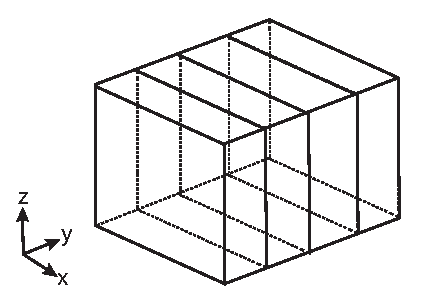
\includegraphics{Figures/2D_slices}
\decoRule
\caption[2D Sclices]{2D slices of the volume.}
\label{fig:2dslices}
\end{figure}
On modern graphics workstations, the complete process of interpolating texture coordinates and reconstructing texture values is incorporated into the scan-conversion process and done completely in hardware. Because texture mapping is such a common application, these routines are well-optimized and highly efficient.
To simulate ray casting using texture mapping, we have to slice the volumetric data set into parallel slices, and the use these slices as texture images to texture-map the projections of the sliced onto the image plane. To composite the slices, we can use the blending operations provided by the OpenGL graphics library. As it happens, one of the standard operators provided is exactly the compositing operator used in ray casting. Since compositing is also fully hardware-assisted, it is also very fast.
\begin{figure}[th]
\centering
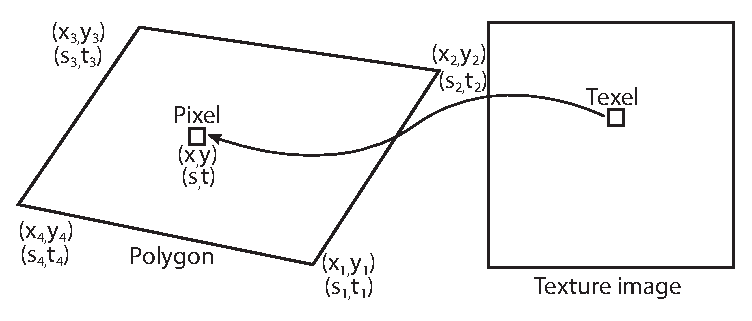
\includegraphics{Figures/2dtexmapping}
\decoRule
\caption[2D texture mapping]{Calculating color and opacity of a pixel inside a texture-mapped polygon.}
\label{fig:2dtexture}
\end{figure}

There are two ways to deal with varying viewpoints.

The first one is to create slice images for the given data set in a pre-processing step and uses different projection matrices to create arbitrary-viewpoint images of these slices. This is fast, since the (expensive) step of slice creation has to be done only once. On the other hand, image quality suffers because the views of all slices will be distorted due to the projection onto the image plane. In the extreme case of the view direction being parallel to the slices, there will be no image at all.

The second way is to create slices which are always orthogonal to the viewing direction. This results in optimal image quality, but it means that the slice stack has to be re-generated for each new image. Furthermore, arbitrary ("oblique") slices through a cuboid are generally not square or rectangular, and can be anything from triangles to hexagons.

\begin{algorithm} \caption{Volume Rendering using 2D Texture Mapping Algorithm} 
\label{alg:tex2dmapping}
\begin{algorithmic}[1]
\Require $N$ the number of slices, $\vec{v} $ the view direction
\State Load the data $\mathcal V(x,y,z) \gets data$ 
\State create the slices $s_i \in \mathcal V$ with each normal $\vec{n_i} \parallel \vec{v}$
\State Turn off the Depth test 
\State Enable the Blending 

\ForEach {$s_i \in \mathcal V $ form back to front}
\State $Texture \gets s_i$
\State create a polygon $p$ corresponding to the slice $s_i$
\State Assign texture coordinates to four corners of the polygon
\State Render and blend the polygon (alpha blending) 
\EndFor

\end{algorithmic}
\end{algorithm}

\paragraph{3D Texture mapping}
To allow interactive generation of view-orthogonal slices, a special hardware technique has been developed. This is a generalization of texture-mapping to three-dimensional textures, appropriately called "3D texturing."
As seen in Figure \ref{fig:2dtexture}, 2D texture-mapping interpolates two additional coordinates (s, t) across a polygon's interior. In 3D texture-mapping, three additional coordinates (s, t, r) are interpolated. To determine a pixel's color and opacity, these three coordinates are used as indices into a three-dimensional image, the 3D texture, see Figure \ref{fig:3dtexture}. To reconstruct texture values, tri-linear interpolation is used.

3D textures allow direct treatment of volumetric data. Instead of generating a set of two-dimensional slices in a pre-processing step, the volumetric data is directly downloaded into the graphics hardware, and is directly used to calculate color and opacity values for each pixel covered by a rendered primitive.

\begin{figure}[th]
\centering
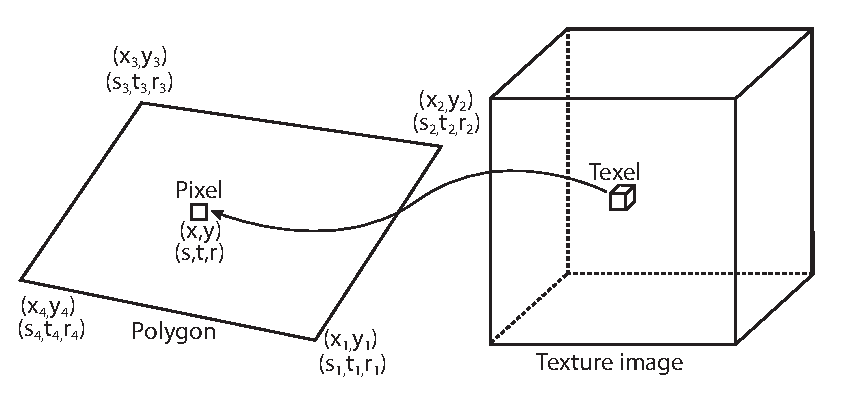
\includegraphics{Figures/3dtexmapping}
\decoRule
\caption[3D texture mapping]{Calculating color and opacity of a pixel inside a texture-mapped polygon using 3D texture.}
\label{fig:3dtexture}
\end{figure}


To generate oblique slices using 3D texturing, one only has to calculate the vertices of the slice, and then to generate the correct 3D texture coordinates for those vertices, see Figure \ref{fig:cubeSlice}. Then these coordinates are passed to the graphics library, and the graphics library will render the projection of the slice onto the image plane, using tri-linear interpolation to reconstruct each pixel's color and opacity values.

\begin{figure}[th]
\centering
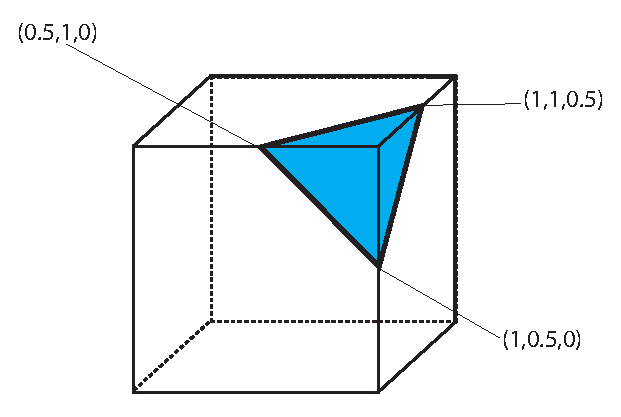
\includegraphics{Figures/cubeSlice}
\decoRule
\caption[3D Cube slice]{Calculating vertex coordinates and texture coordinates for an oblique slice. In this figure, the vertex and texture coordinates are identical.}
\label{fig:cubeSlice}
\end{figure}

\subsubsection{Raycasting}
Volume raycasting computes a 2D image from the 3D volumetric data set.The basic goal of ray casting is to allow the best use of the three-dimensional data and not attempt to impose any geometric structure on it. It solves one of the most important limitations of surface extraction techniques, namely the way in which they display a projection of a thin shell in the acquisition space. Surface extraction techniques fail to take into account that, particularly in medical imaging, data may originate from fluid and other materials which may be partially transparent and should be modeled as such. Ray casting doesn't suffer from this limitation. This algorithm can be split in four main steps (see Figure \ref{fig:rayasting}) :
\begin{itemize}

\item \textbf{Ray casting}. For each pixel of the final image, a ray of sight is shot ("cast") through the volume. At this stage it is useful to consider the volume being touched and enclosed within a bounding primitive, a simple geometric object (usually a cuboid) that is used to intersect the ray of sight and the volume.

\item \textbf{Sampling}. Along the part of the ray of sight that lies within the volume, equidistant sampling points or samples are selected. In general, the volume is not aligned with the ray of sight, and sampling points will usually be located in between voxels. Because of that, it is necessary to interpolate the values of the samples from its surrounding voxels (commonly using trilinear interpolation).

\item \textbf{Shading}. For each sampling point, a transfer function retrieves an RGBA material colour and a gradient of illumination values is computed. The gradient represents the orientation of local surfaces within the volume. The samples are then shaded (i.e. coloured and lit) according to their surface orientation and the location of the light source in the scene.

\item \textbf{Compositing}. After all sampling points have been shaded, they are composited along the ray of sight, resulting in the final colour value for the pixel that is currently being processed. The composition is derived directly from the rendering equation and is similar to blending acetate sheets on an overhead projector. It may work back-to-front, i.e. computation starts with the sample farthest from the viewer and ends with the one nearest to the viewer. This work flow direction ensures that masked parts of the volume do not affect the resulting pixel. The front-to-back order could be more computationally efficient since, the residual ray energy is getting down while ray travels away from camera; so, the contribution to the rendering integral is diminishing therefore more aggressive speed/quality compromise may be applied (increasing of distances between samples along ray is one of such speed/quality trade-offs).

\end{itemize}

\begin{figure}[th]
\centering
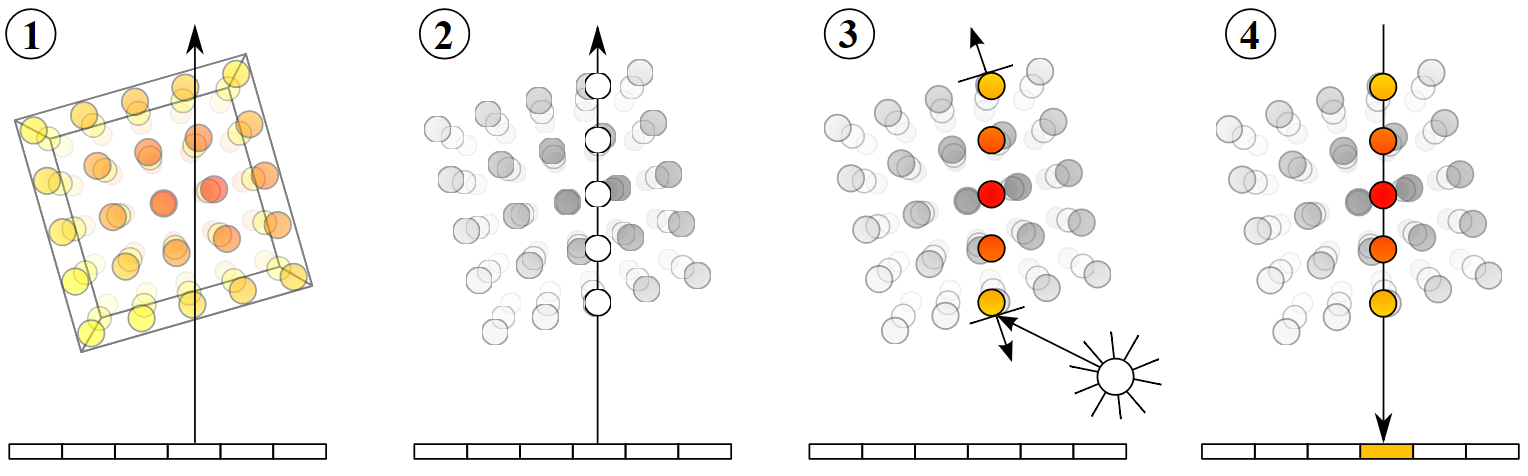
\includegraphics[width=\textwidth]{Figures/raycasting}
\decoRule
\caption[Volume raycasting]{ The four steps of the volume raycasting algorithm  }
\label{fig:rayasting}
\end{figure}

\subsection{Surface-fitting}


\section{Occlusion management strategies}



\subsection{Transfer Function}

A transfer function (TF) maps volumetric data to optical properties
and is part of the traditional visualization pipeline: data acquisition,
processing, visual mapping, and rendering. Volumetric data is
considered to be a scalar function from a three-dimensional spatial
domain with a one-dimensional range (e.g., density, flow magnitude,
etc.). Image generation involves mapping data samples through the
TF, where they are given optical properties such as color and opacity,
and compositing them into the image.
A TF simultaneously defines which parts of the data are essential
to depict and  how to depict these, often small, portions
of the volumetric data. Considering the first step, a TF is a special,
but important, case of a segmentation or classification. With classifi-
cation, certain regions in a three-dimensional domain are identified
to belong to the same material, such as bone, vessel, or soft tissue,
in medical imaging. A plethora of classification and segmentation
algorithms have been developed over the last decades, with semiautomatic
approaches often tailored to specific application scenarios.
Segmentation algorithms can be quite intricate since information
from the three-dimensional spatial domain and the one-dimensional
data range are taken into account. TFs in their basic form are, on the
other hand, restricted to using only the data ranges. In comparison
with general classification algorithms, this characteristic makes a
TF less powerful with respect to identifying relevant parts of the
data. The advantage of a TF is, however, a substantial performance
gain as classification based on the one-dimensional data range reduces
the complexity tremendously. This gain is the result of the
three-dimensional domain being typically two orders of magnitude
larger than the small data range. Histograms are an example of discarding
potentially complex spatial information and aggregating
only the data values to binned-frequency information. In the same
spirit, TFs classify interesting parts of the data by considering data
values alone. The second functionality of a TF deals with specifying
optical properties for portions of the data range previously identified
as being relevant

The transfer functions can be classified according to different criteria. Some of the most important are:

\begin{itemize}
\item \textbf{The dimension: } The one-dimensional TF classifies the scalar data value, $d$, and subsequently maps the material to an optical property for rendering: $ \textbf{q}(d)=\textbf{V}(\textbf{M}(d))$ where $\textbf{M}(.)$ is the material classification function and $\textbf{V}(.)$ is the
visual mapping of the material. One-dimensional TFs are adequate in many cases of simulation data where measurement noise is low or even non-existent where different materials of interest have few overlapping intensity
ranges \cite{4303986}. One-dimensional TFs are often the first tool available in software packages providing volume rendering, as they are relatively easy to comprehend for the novice or occasional user. Practically all production
visualization software, such as ParaView by \cite{paraview},
 VisIt by \cite{Childs:SciDAC2011}, 
or ImageVis3D by {\cite{Fogal2010Tuvok}}, support 1D TF editors.

\begin{figure}[th]
\centering
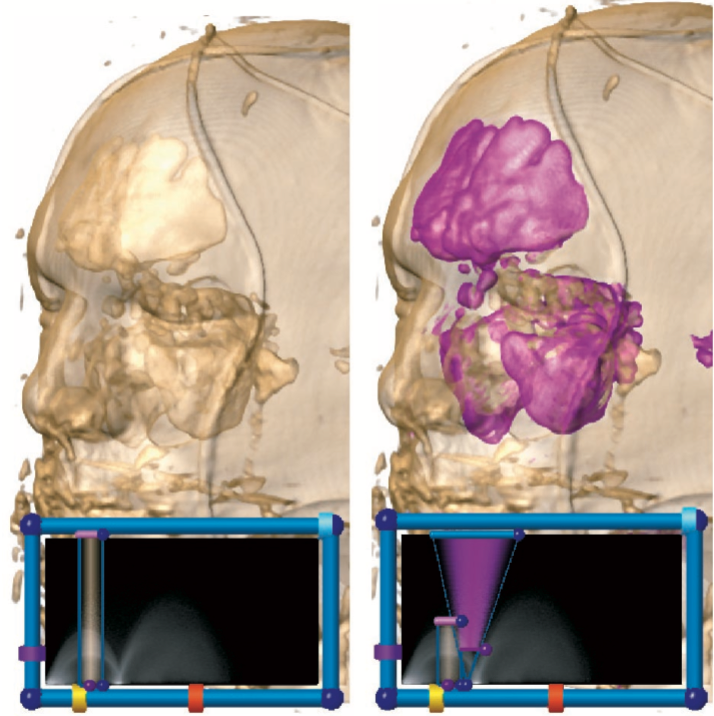
\includegraphics[width=\textwidth]{Figures/2dtf}
\decoRule
\caption[2D transfer Function]{ The two-dimensional TF editor widgets allow the user
to more precisely control the classification power of the 2D TF.
The triangular widget can also be skewed to better fit the desired
classification domain (\cite{1021579}) }
\label{fig:tf2d}
\end{figure}

Multidimensional TFs are used for Multidimensional data. If the user has to manipulate the TF definition directly, moving beyond
2D TFs immediately poses significant challenges in terms of
user interfaces and cognitive comprehension (\cite{1021579}). Much research and
work on Multidimensional TFs is, therefore, related to various forms of automation
and advanced user interfaces. Typical approaches include dimensional reduction, clustering
and grouping, machine learning, and various user interface
approaches such as parallel coordinates by \cite{5742368} or direct slice or volume
view interaction. 

\begin{figure}[th]
\centering
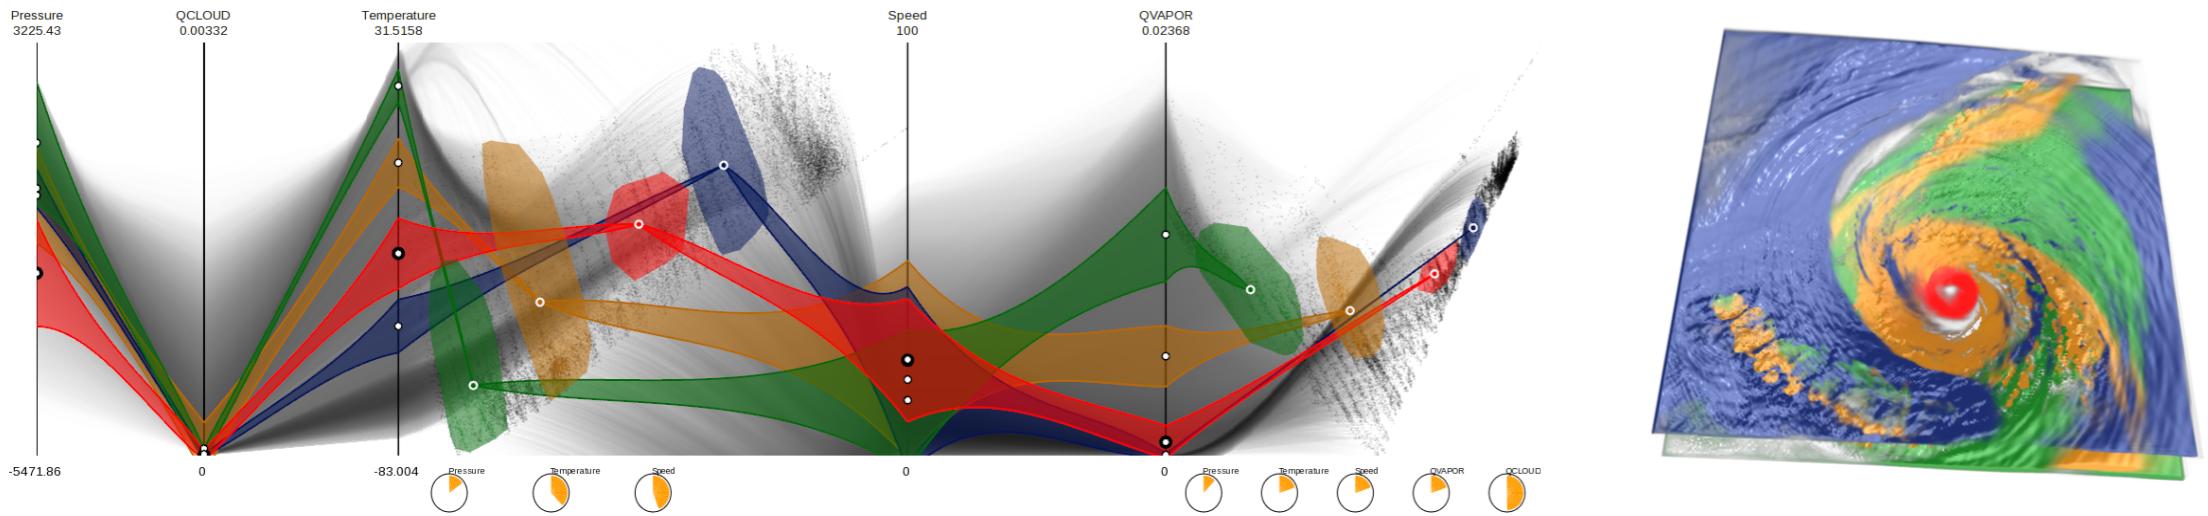
\includegraphics[width=\textwidth]{Figures/mdtf}
\decoRule
\caption[Multidimensional transfer Function]{ Parallel coordinates with embedded multidimensional scale plots for editing multidimensional TFs(\cite{5742368}) }
\label{fig:tfmd}
\end{figure}


\item \textbf{The automation}: The automation includes techniques such as adapting presets, semi-automatic, automatic, and supervised machine learning. Volume rendering has established itself as
a powerful visualization tool in many domains, but the necessary
design of TFs is a time consuming and tedious task. Consequently,
a significant amount of work is dedicated to the automatic and semiautomatic generation of TFs. 

\item \textbf{The aggregated attributes} : Conceptually, the introduction of additional quantities in the TF definition makes it possible to discriminate more parts in a dataset. Histogram clustering helps to reduce the degrees of freedom in designing a TF. As an illustration, \cite{5887324} propose modeling the
histogram space using a Gaussian mixture model. An elliptical TF
is assigned to each Gaussian, and the user interaction is simplified in order to edit the parameters of these ellipsoids.  

\end{itemize}

\subsection{Segmentation}

\subsection{Deformations and Focus + Context}

An interactive lens is a lightweight tool to solve a localized visualization problems by temporarily altering a selected part of the visual representation of the data~\cite{CGF:CGF12871}. Using this lens approach, we propose an interactive volume deformation based on GPU accelerated ray-casting to free a designated target from local occlusion while keeping the global context.

A lens is a parameterizable selection according to which a base visualization is altered. Typically, a lens is added to a visualization to interactively solve a specific localized problem. This property is very interesting with the aim of providing a focus+context solution to occlusion in volume rendering. Lenses can have different geometric properties not only defining their appearance, but also determining the selection, which is the subset of the data where these lenses take effect. The major geometric properties of a lens are shape, position, and size as well as the orientation.
The shape of a lens is usually chosen to fulfill the requirements of the application and is strongly linked to the lens function. Most virtual lenses are circular~\cite{1648236} or are rectangular~\cite{Kincaid:2010:SFA:1907651.1907963} as the real-world ones (magnifying glass, windows). Our lens has also a circular shape in order to remind its magnifying property. Some lenses, such as the  JellyLens~\cite{Pindat:2012:JCA:2380116.2380150} and the smart lenses~\cite{Thiede2008} can adapt their shape automatically according to the data. 
The position and the size parametrization can increase the flexibility of an interactive lens.
Modifying this position or size will set its focus on a different part of the data according to the user's interest. It is possible to update automatically these parameters in order to guide the user toward interesting events in the data~\cite{Tominski:2011:ECU:2336207.2336211}, or adjust the lens position according to predefined paths as the Routelens~\cite{Alvina:2014:RER:2598153.2598200} does. With this mind, our lens updates automatically its properties once a target has been selected. This allows a smooth transition towards an unobstructed and magnified area of interest. 

Lenses for volume visualization face challenges mainly related to spatial selection and occlusion. Wang et al. addressed these issues by proposing the Magic Lens~\cite{1532818}. This Magic Lens renders the obstructions with higher transparency and magnifies volumetric pre-computed features interactively or automatically in a pre-segmented dataset. In addition to interactively magnifying areas and objects of interest, our lens frees them from obstruction and allows local modification of the camera to see the target under other perspectives. Tong et al. proposed the GlyphLens~\cite{7539643} that removes the occluding glyphs by pulling the glyphs aside through the animation, but this tool is only well suited for systems where 3D volumetric dataset are visualized using glyphs. Lenses can create discontinuities between their inner part and the rest of the volume. Deformation can be a solution to this discontinuity issue.   




 \cite{Hsu:2011:RFM:2070781.2024165} developed a framework that can generate non-linear sampling rays that smoothly project objects in a scene at multiple levels of detail onto a single image. Such a technique requires a lot of computational time to render a single image from features of interest at different scales, see figure \ref{fig:multiscale}.This  multiscale rendering framework consists of a sequence of pinhole cameras, each of which captures a view of interest at a particular scale. The camera rays for each pixel in the final projected image are generated based on a user-defined image mask which specifies the interesting regions in each view.  The camera rays non-linearly cast through all scales of interest. Since the camera rays in the model are bent coherently and march consistently, the objects projected on the image are continuous in both image-space and object-space. 
 Their method starts by setting up several pinhole cameras for viewing different scales of interest, utilizing most users’ ease and familiarity with manipulating ordinary pinhole cameras. Each camera produces an image of its view. In order to combine all such views to form a single multiscale image, a user-specified image mask is used to indicate regions of each view that the user would like to show in the final image. In other words, every camera projects only part of its view onto the final image space, based on a corresponding image mask. In order to ensure consistency while projecting different camera
viewpoints onto different parts of the image, we force all camera rays to originate from the first camera, which is the one that has the largest scale of view. The rest of the cameras define intermediate
points that camera rays must pass through in order, from the largest to smallest scales. They use B\'ezier curves to connect the nearclipping planes of two successive cameras.

  The rays are bent gradually from one scale to another to maintain object-space continuity as well as image-space smoothness. The multiscale camera can also achieve a focus+context effect, a technique frequently used in many visualization applications. Finally, we show that it can potentially create pictures that mimic artistic or impossible views of objects or scenes like the kind made by the artist M. C. Escher. 
 
\begin{figure}[th]
\centering
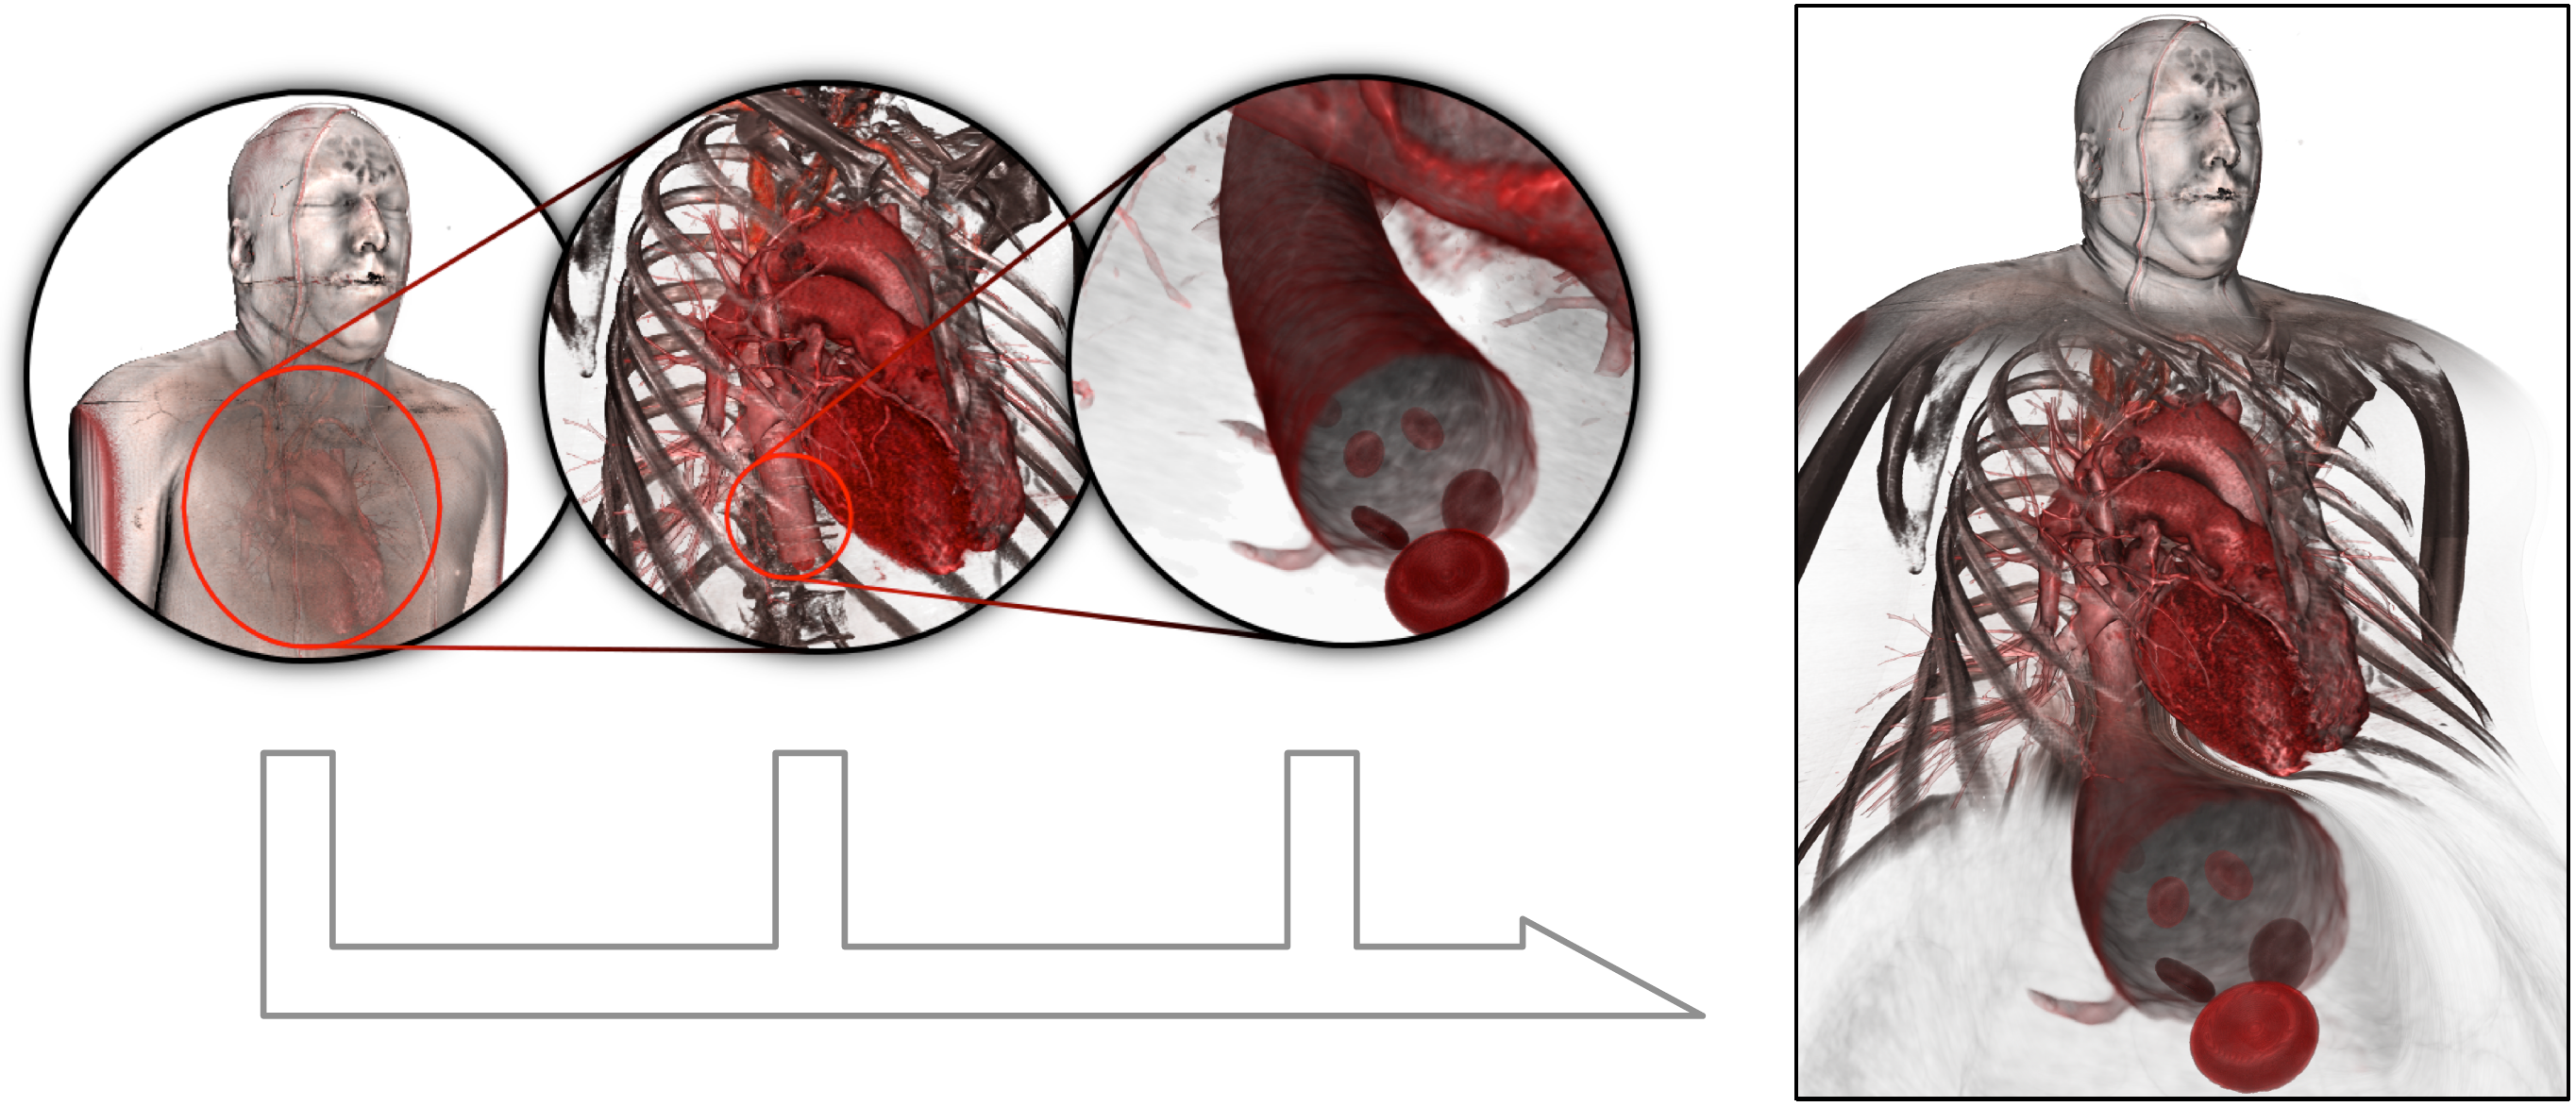
\includegraphics[width=\textwidth]{Figures/multiscale3d}
\decoRule
\caption[ multiscale ]{ A Rendering Framework for Multiscale Views of 3D Models. A continuous multiscale view (right) of a volumetric human body dataset shows three different levels of detail (left three) in a single image. The image on the right is directly rendered with our multiscale framework.}
\label{fig:multiscale}
\end{figure} 
 
  Bruckner and  Groller~\cite{4015467} proposed exploded view for volume data by partitioning the volume into several segments (figure \ref{fig:exploded}). Basically, in an exploded view the object is decomposed into several parts which are displaced so that internal details are visible. This does not only give an unobstructed view on the focus but also potentially reveals other interesting information, such as
cross-sections of the split object. The advantage of exploded views is that they simultaneously convey the global structure of the depicted object, the details of individual components, and the local relationships
among them. A Force-directed layout approach is used to arrange three-dimensional objects
in such a way that they do not occlude another object, but with as little displacement as possible. Four forces are used. \textbf{The Return force } is an attractive force that tries to move the parts towards
their original location. The force $F_r$ is realized as a logarithmic spring:
 \[ F_r=c_{r}\ln(||r||)\cdot \frac{r}{||r||} \] 
 where $r$ is the vector from the vertex's current position to its original location and $c_r$ is a constant factor.
 \textbf{The Explosion force} drives the specified parts away from our selection object. The explosion point is also weighted according to the size of the region corresponding to an octree node. Each explosion point exerts a force $F_e$ on every part $P_i$:
  \[ F_e=  \frac{c_e}{e^{||r||} } \cdot \frac{r}{||r||} \]
  where $r$ is the vector from the explosion point to the closest point of the part geometry of $P_i$ and $c_e$ is a scaling factor.
   \textbf{The Viewing force} is a view-dependent force which attempts to arrange parts so that they do not occlude the selection for the current viewing transformation. The force $F_v$ is:
   \[ F_v=  \frac{c_v}{||r||} \cdot \frac{r}{||r||} \] 
   where $r$ is the vector from the closest point along the viewing ray to the center of the body and $c_v$ is a scaling factor.
   \textbf{The Spacing force} prevents clustering of parts, we also add a
repulsive force $F_s$. For a part $P_i$, the spacing force exerted by another part $P_j$ is:
\[ F_s=  \frac{c_s}{||r||^2} \cdot \frac{r}{||r||} \] 
where $r$ is the vector from the center of $P_j$ to the center of $P_i$ and
$c_s$ is a constant scaling factor. 
\begin{figure}[th]
\centering
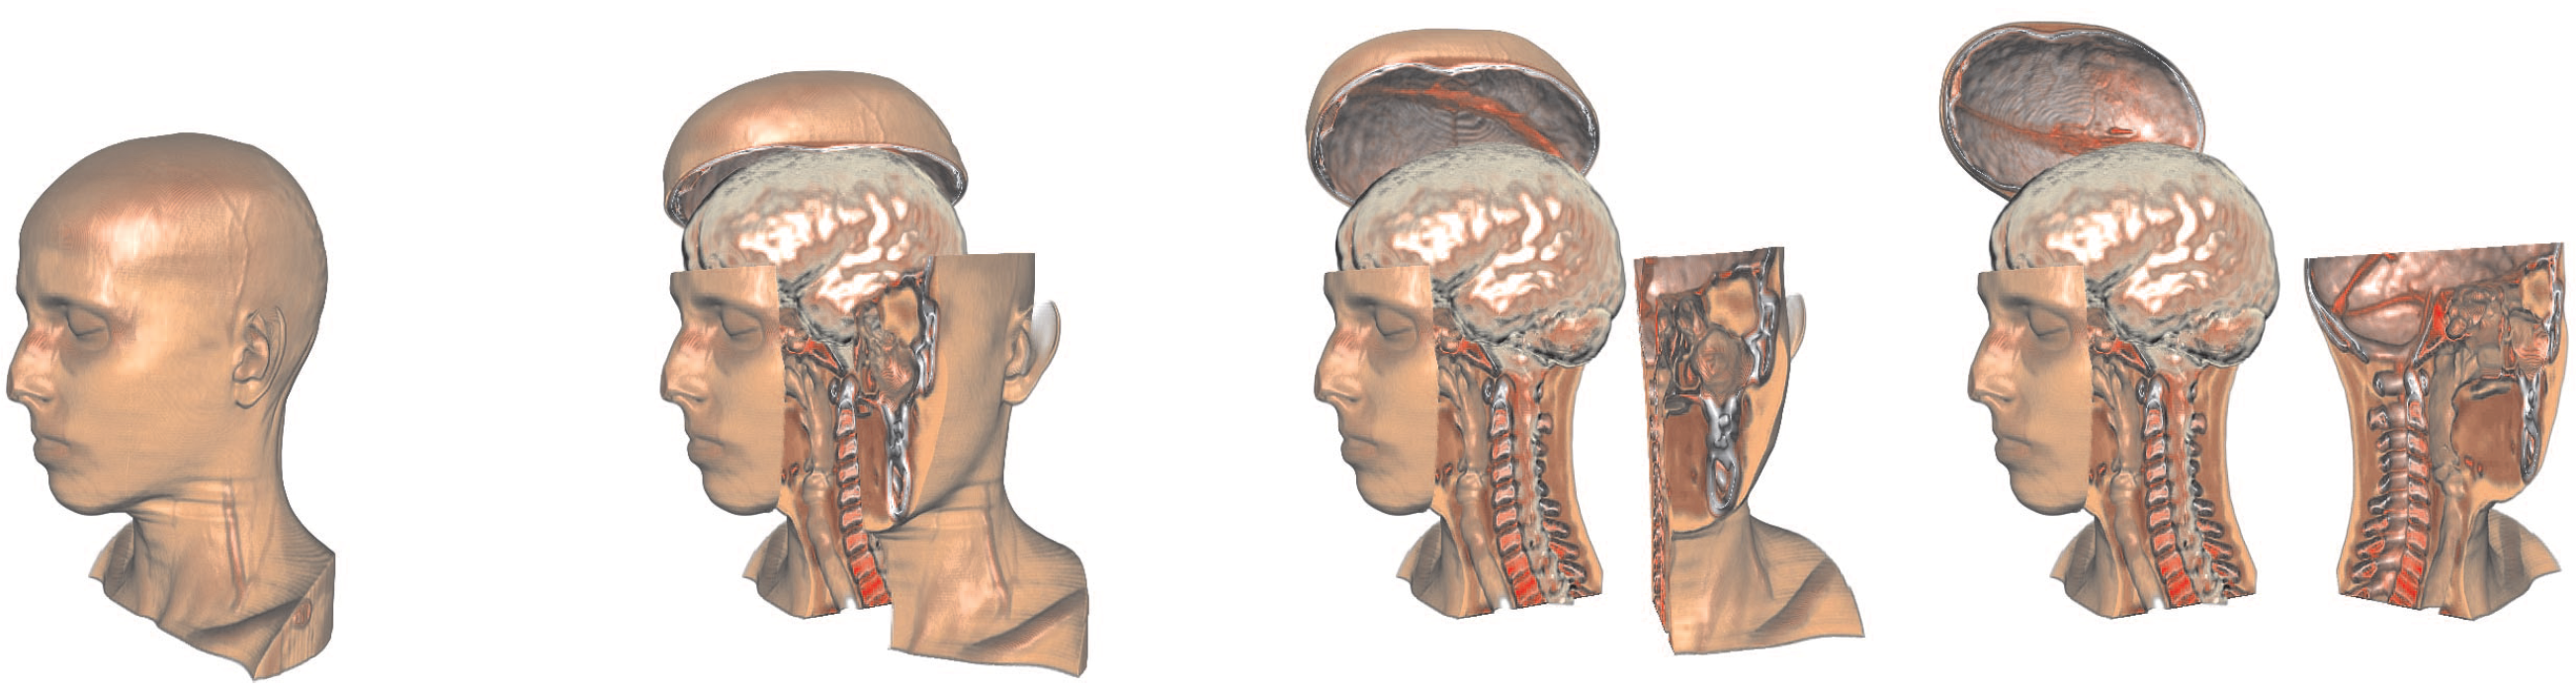
\includegraphics[width=\textwidth]{Figures/explodedview}
\decoRule
\caption[ Interactive exploded-view]{ Interactive exploded-view illustration of a human head with increasing degrees-of-explosion. Two hinge joints are used to constrain part
movement}
\label{fig:exploded}
\end{figure}
  
 
  
   McGuffin et al.~\cite{1250400} performed deformations using peeling to see hidden parts of the data. However, these techniques have the disadvantage of removing potentially important surrounding contextual information while trying to solve the local occlusion. 
 
 
Deformations can reveal predefined features in the dataset by taking into account the precomputed segmentation. Tong et al. proposed a deforming Lens which moves streamlines to observe the inner part of streamline bundles~\cite{7332955}. 


 Correa et al. proposed a framework~\cite{Correa:2007:IDD:1313046.1313163} allowing the users to physically or actively manipulate the geometry of a data object. Some studies performed deformations using surgical metaphors like ~\cite{4069230,Correa:2006:FAV:1187627.1187827} to see hidden parts of the volume, see figure \ref{fig:cut}. They propose a feature-based technique for manipulating volumetric objects for illustrative visualization, and describe a GPU-based implementation that enables interactive specification and their rendering.
Inspired by medical illustrations that frequently
depict the results of manipulation with tools such as peelers,
retractors and pliers, this system allows the specification of manipulation
through a collection of procedurally-defined manipulation operators.

\begin{figure}[th]
\centering
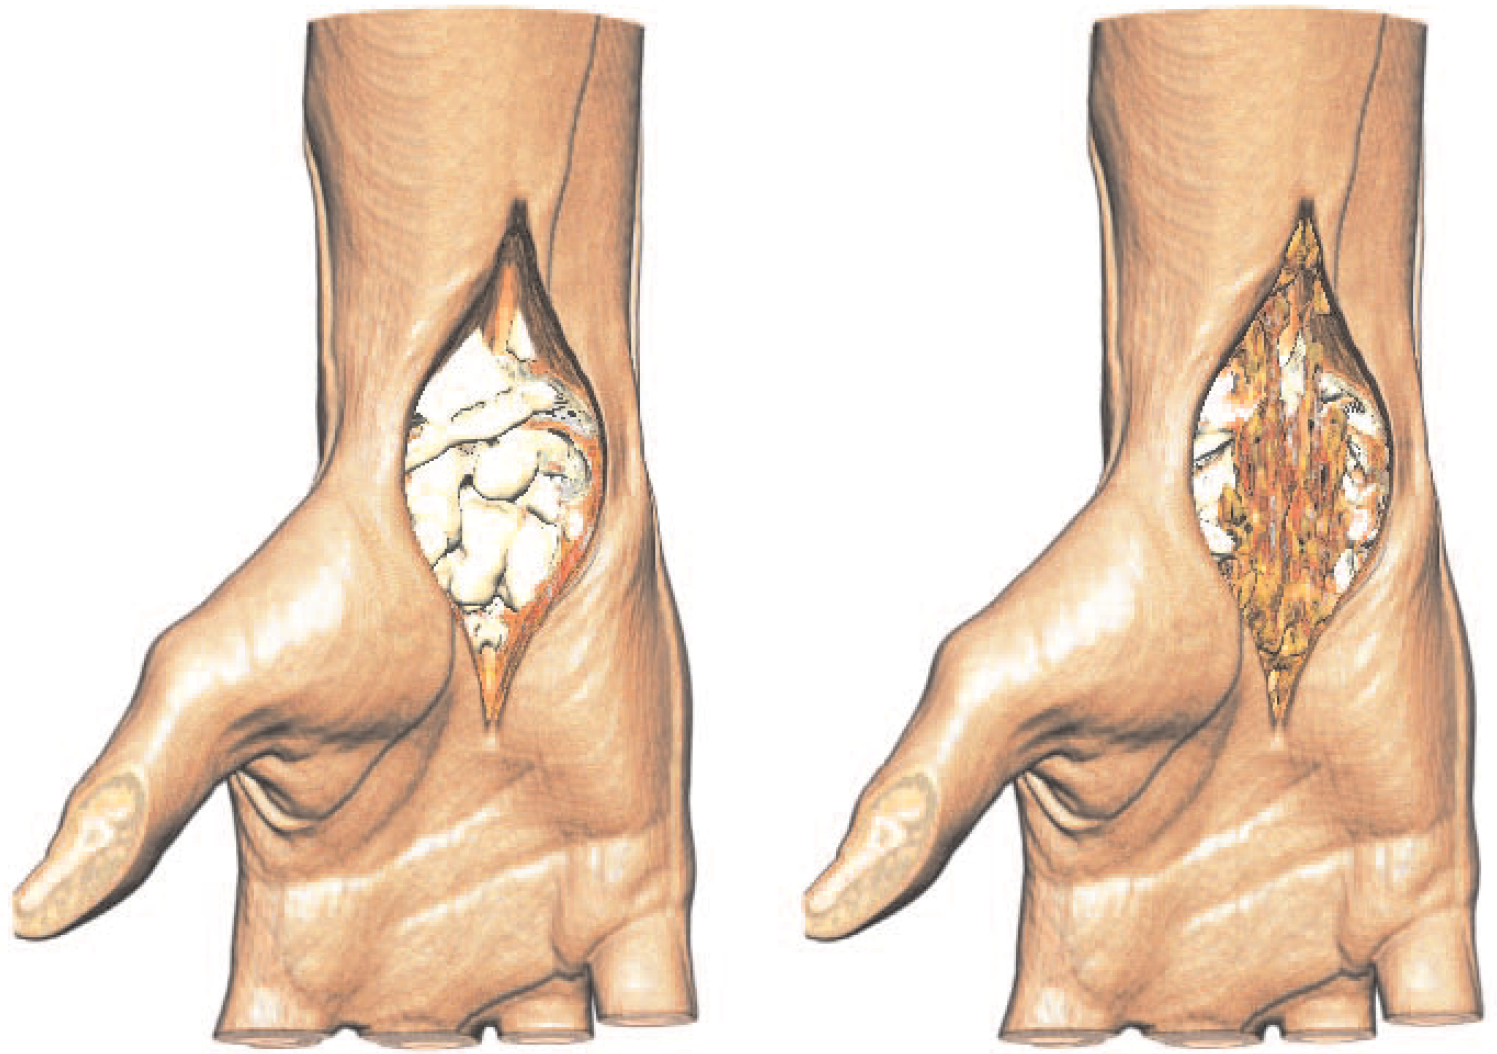
\includegraphics[width=\textwidth]{Figures/cut}
\decoRule
\caption[ Feature Aligned Volume Manipulation]{ A feature-aligned retraction applied to a human hand data set, showing bones (left) and vessels (right)}
\label{fig:cut}
\end{figure}

  \begin{figure}[th]
\centering
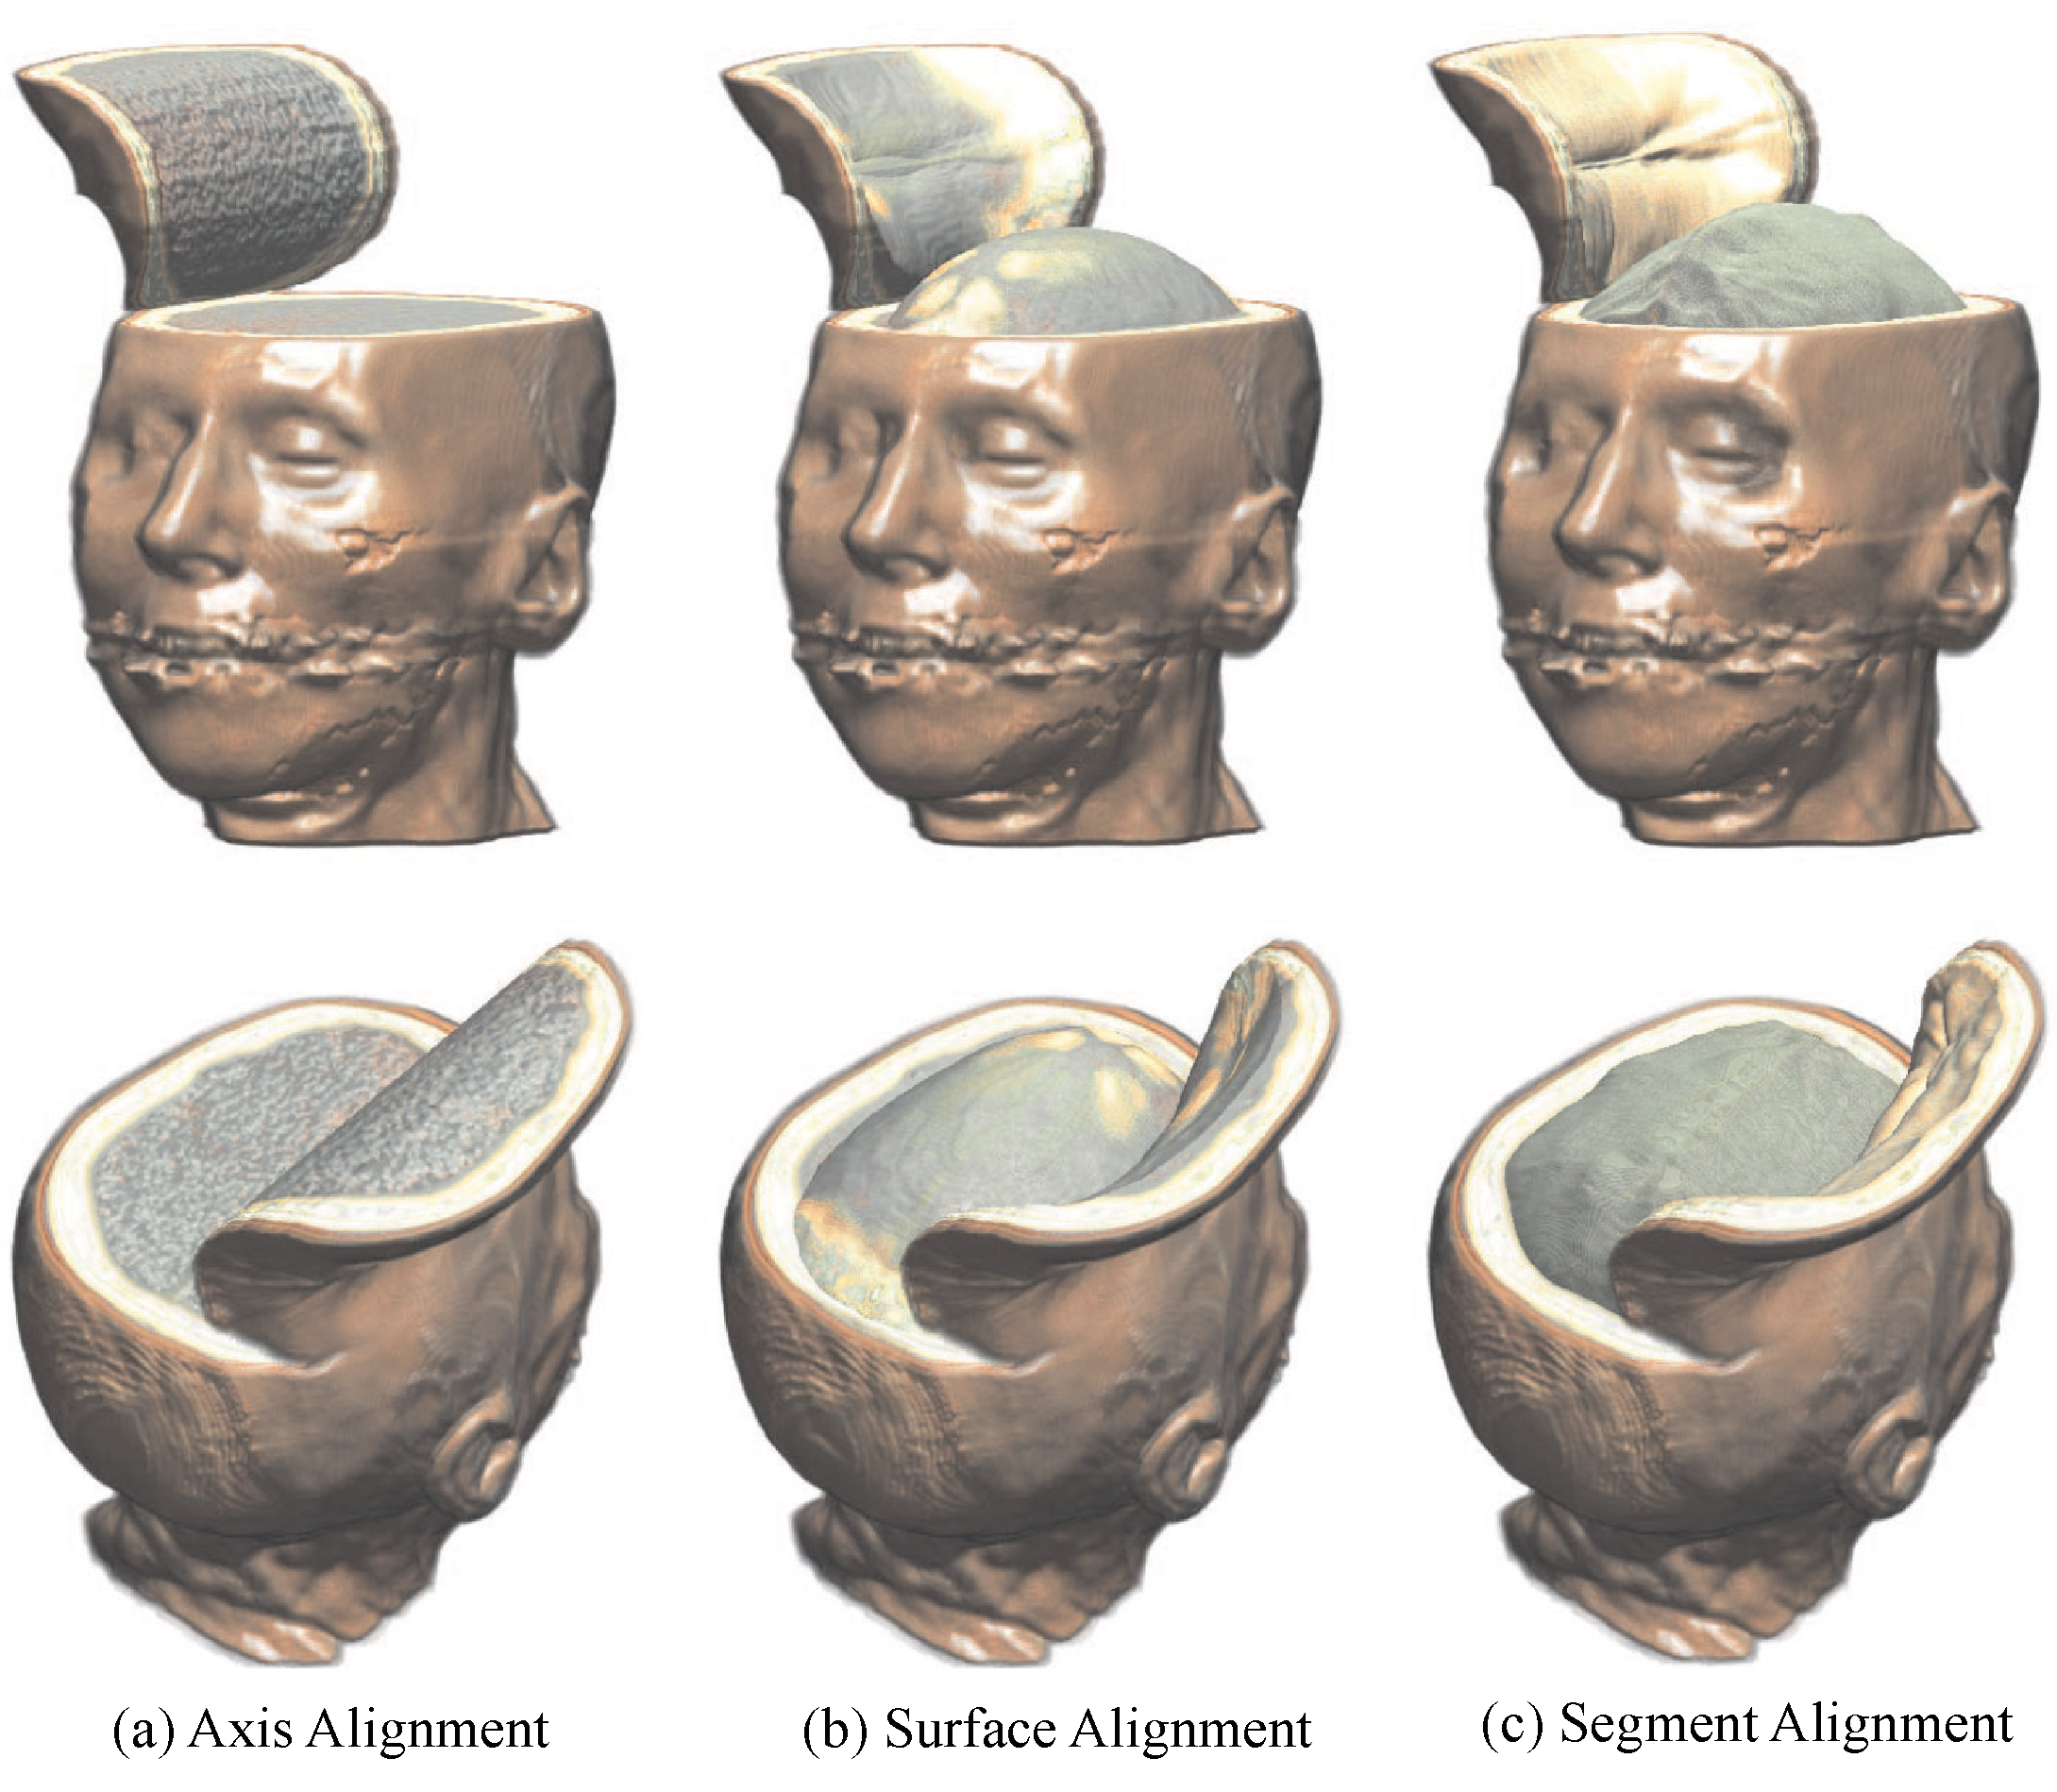
\includegraphics[width=\textwidth]{Figures/peel.pdf}
\decoRule
\caption[ Feature Aligned Volume Manipulation]{ An example of different types of alignment. (a) Axis aligned peel. Note how the peeled layer is thick and flat, since it is aligned with
an orthogonal axis. (b) Surface aligned peel, aligned with a computed
distance field. Notice how it approximates a surface. (c) Segment
aligned peel, based on segmentation, which is more accurate. Note
that in the feature based alignment (b) and (c) the peel is thin and
rounded.}
\label{fig:peel}
\end{figure}

 Correa et al. introduced two feature-based methods, namely surface alignment and segment alignment for modeling and rendering illustrative manipulation, and compare them with the traditional axis alignment method, see figure \ref{fig:peel}. They devise a method for estimating accurate normals along the surface of cuts
and dissections while maintaining continuous normals, which allows
us to obtain correct shading of the object being manipulated, opaque
or translucent. The four operators proposed in this framework are the following:
\begin{itemize}
\item Peeler: The peeler simulates peeling or cutting of the outer layers
of a volumetric model. Different parameters
of the peeler, such as thickness of the cut and the angle of bending of
the peeled layer, can be manipulated interactively to obtain different
illustrative effects.
\item Retractors: In the context of surgical illustration, retractors are tools used to spread organs or bones, or to hold back soft tissues such as
skin. In the context of illustration, they are useful for illustrating the
access to the internal organs.
\item Pliers: Pliers are tools used to grasp tissue and pull it or poke it into the volumetric object. The operator parameters include the shape of
the displacement and the radius of influence which specifies how the
displacement propagates through the volume.
\item Dilator: Dilators are used to gain access into narrow regions, cuts
or vessels. They essentially scale the region from the inside typically
by blowing air, to increase the visibility or accessibility of the region.
When applied to volumetric manipulation, dilators have a similar effect
to that of volumetric magic lenses (~\cite{1532818}).
\end{itemize} 
However this framework do not offer tools for local manipulation and exploration inside the cut, which allows perceiving a target under a different perspective while keeping the global context. 


\section{Volume rendering in Virtual Reality and Augmented Reality}

\subsection{ Remote volume rendering}

Volumetric data exploration with direct volume rendering technique is of great help to visually extract relevant structures in many fields of science: medical imaging ~\cite{ljung_full_2006}, astrophysics and more recently in baggage inspection. To leverage this knowledge extraction, many techniques have been developed. 

In this section, we detail existing ones with volume visualization, transfer function, direct voxel manipulation, and focus plus context interaction.
Volume visualization can be done with geometric rendering system which transforms the data into a set of polygons representing an iso-surface. The contour tree algorithm ~\cite{carr_computing_2000} and other alternatives such as branch decomposition ~\cite{pascucci_multi-resolution_2004} are usually used to find these iso-surfaces. According to H. Guo ~\cite{guo_local_2013}, contour trees algorithms are vulnerable to noises, which can be problematic in baggage inspections since dense materials (e.g. iron) cause noises by reflecting the X-rays. For this reason we used the volume rendering technique; Chen et al. provide a review of existing techniques ~\cite{chen_3-d_2000}.
In order to investigate volumetric dataset, one can use the Transfer Function (TF). In practice, it maps the voxel density with a specific color (including its transparency). Transfer function can be 1D, 2D or nD and are of great help to isolate structures of interest in volumetric data ~\cite{kniss_multidimensional_2002}. Thanks to the color blending process, suitable transfer function can also reveal iso surface or hide density to improve the volumetric data visualization. The setup of this transfer function remains complex, but some automatic systems provide solution thanks to data analysis ~\cite{correa_size-based_2008} ~\cite{sereda_visualization_2006} ~\cite{patel_moment_2009} or user interactions ~\cite{guo_wysiwyg_2011}. Since our users have a limited knowledge on volume rendering, we developed new interaction techniques with sufficient abstraction level regarding technical constraints. These techniques will be detailed in this paper. As an example, we investigated predefined transfer functions with smooth transitions when changing their setup to reduce disruptive animation effects ~\cite{tversky_animation:_2002}.
Since graphic card power never stops to improve, new techniques allow the direct manipulation of the voxels which composes the volume to be displayed. Color tunneling introduced a set of interactions (lock, Brush, Dig) to explore 2D and 3D dataset composed of pixels of voxels ~\cite{hurter_interactive_2014} with point based rendering techniques ~\cite{sainz_point-based_2004} . Histomage also provides direct manipulation of pixels thanks to a histogram which can be used as a new selection and pixel modification tool ~\cite{chevalier_histomages:_2012}. Other interactive systems investigated pixel exploration with a lens as a focus plus context technique ~\cite{elmqvist_color_2011} ~\cite{hurter_moleview:_2011}. Our work provides additional interaction techniques with pixel based techniques ~\cite{hurter_interactive_2014} to address occlusion issues, focus and context awareness, reversibility of the actions, and continuity.  
\chapter{User Study: Interactive exploration of 3D scanned baggage} % Main chapter title
\label{DesignStudy}

\section{ Preliminary user study }
During the first months of my thesis, I carried out a user study of eye tracking devices to build interactive systems for Air Traffic Controllers. \textbf{ The purpose of that was quite similar to the one I describe in this chapter: \textit{Provide fluid and fast interactions to ease the tasks of the users.} }


While the mouse is the main input device for interacting with different screens, many alternatives do exist. In this work, we reported our exploratory study with the usage of
eyes as a new input device for Air Traffic Control systems. Our investigations, based on a user-centered design, included a study of the activity, a classification of interaction
techniques based on eye tracking systems, and finally a working prototype with the evaluations of the developed interaction techniques. Our goal was to investigate gaze usages
as a means of interaction, and give recommendations for future development of Air Traffic Control systems.


The activity of air traffic control is complex. Operators use many interactions techniques with dedicated IT systems to ensure the traffic flow with respect of security and
optimization concerns. Air traffic activities is constantly evolving. Air traffic
controllers, responsible for ensuring the safety and the fluidity of air traffic, have to deal with more and more information that could cause a significant increase in their
workload. However, whether in control tower, approach or even in En-Route control center, air traffic controllers have many tools in addition to the radar screen. Their
workspace is thus the scene of an accumulation of interaction devices (mainly mice and touchscreens).

\subsection{ Contextual observations }

In the following, we briefly describe the controller tasks within the three previously defined contexts. The activity of en-route and approach controllers [16] is mainly to maintain a safe distance between aircraft, and to guide them with traffic fluidity concerns. For this, the airspace is divided into sectors, each sector being the responsibility of one controller pair. When a flight goes through an area, controllers guide
the pilot by giving him or her orders (clearances) for heading, speed or altitude, until the flight reaches an adjacency sector where other controllers will be in charge of
this aircraft. In a typical environment, two controllers are seated in front of a control position, specially designed to support their job. A traditional position includes a set of
main subsystems: two radar screens (one for each controller), paper strips shared by both controllers (for systems using the strips) displayed on a horizontal table.

\subsection{ limiting factors }

With current systems, controllers are able to perform many
different types of interaction. This allows in particular to
obtain aircraft details, to setup the radar configuration or to
share information with other controllers. During the
observation sessions, we extracted some controllers frequent
interactions with existing systems:
\begin{itemize}
\item pan and zoom to set the radar view configuration,
\item entering a clearance,
\item distance computation between planes using the alidade,
\item display of the separation distance between aircraft,
display of velocity speed vectors (position of the aircraft in
3, 6, or 9 minutes).
\end{itemize}

We have identified a number of limiting factors for these
interactions. Although navigation is available in the radar
image (pan and zoom), it still does not allow to see the
calling planes located outside of the displayed area. This
view configuration is done by clicking on the buttons located
in a context menu. Other features are accessible via a toolbar
or a shortcut menu. This is for example the case of the
alidade (measuring the distance between two aircraft), which
is performed by selecting it on the tool bar on the left of the
radar display (Figure 1) and then plotting on the map the line
representing the distance to assess the distance using a drag
with the left mouse button.
In conclusion, many interaction requires the mouse device with
numerous manipulations (reach the mouse, find the menu
location, select the appropriated item, perform selections and mouse drags, etc.)

\subsection{Interactions}
After the brainstorming, we built prototypes (\autoref{e:prototype}) that were
evaluated during a design walkthrough session with 3
confirmed air traffic controllers.

 \begin{figure}
 \centering
	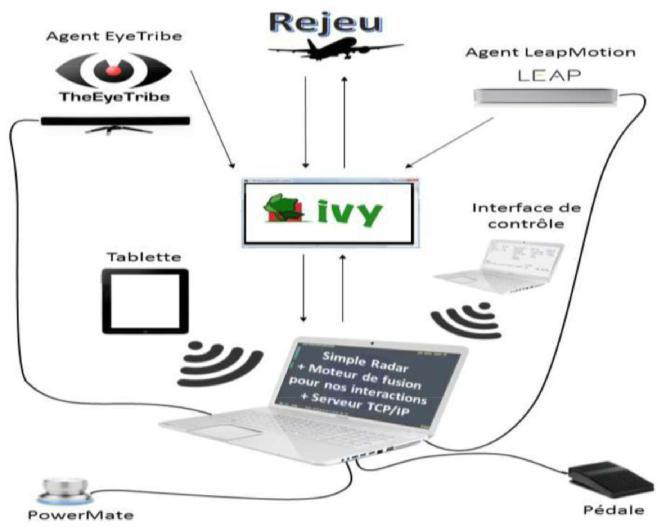
\includegraphics[width=0.95\textwidth]{Figures/prototype.png}
	\caption{ The architecture of the prototype}
	\label{e:prototype}
\end{figure}

\subsubsection{I1: Selection methods}
The selection of an aircraft is the first task an air traffic
controller shall achieve before interacting with it. To do this, different techniques of
interaction are possible and are shown in the following.

\paragraph{I1-1: The mouse (Existing Technic)}

We kept the functioning of this interaction which is already
implemented in existing systems, in order to compare the
eye tracker and the single mouse. (\autoref{e:})


\paragraph{I1-2: The Dwell Time}
The Dwell Time is a technique that allows to change the
state of a target (aircraft in this case) when looked for a
certain period (\autoref{e:selectionState}).

\begin{figure}
 \centering
	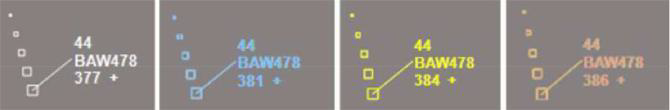
\includegraphics[width=0.95\textwidth]{Figures/selectionState.png}
	\caption{ The different states of an aircraft}
	\label{e:selectionState}
\end{figure}

Our prototype has two buttons, one for the validation and the
other one to cancel a previous validation. The appearance
and size of these buttons have been modified following the
remarks during the design walkthrough sessions. The
buttons are positioned in areas normally without traffic
(\autoref{e:selectionDwell}). The user must look at a plane: it will switch to
blue after a first timer (dwell time, 200ms). Then the user
simply look at the "validate" button for a certain period to
select the aircraft (it changes to yellow). To cancel the
selection of this aircraft, the user must again look at it, then it turns red, and if the user looks at the cancel
button for a certain period, the airplane is deselected (\autoref{e:selectionDwell}).

\begin{figure}
 \centering
	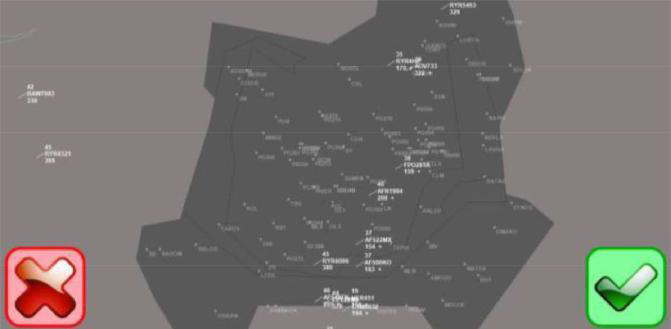
\includegraphics[width=0.90\textwidth]{Figures/selectionDwell.png}
	\caption{ Selection with dwell time}
	\label{e:selectionDwell}
\end{figure}



\paragraph{I1-3: Buttons}
During the brainstorming session, it emerged that the best
option to select an aircraft is to use an external device
(button, keyboard or pedal, etc.). That is why we decided to
include this interaction in the final prototype.

\paragraph{I1-4: Pedal}
This interaction is almost identical to the previous one,
except that it offers the user a button that plays both the role
of the "validate" and the "cancel".

\subsubsection{I2: Function Selection}
The methods of the function selection we implemented,
respond to the needs to obtain information on a plane, and
free the hands.
 
\paragraph{I2-1: Pulldown Menu}
This interaction is similar to the one existing in the current
systems. With a click on an aircraft, users have access to a
context menu offering several features. This interaction has
been developed for the purpose of comparison with the new
methods of selection that we propose (\autoref{e:selectionFunction}).
\begin{figure}
 \centering
	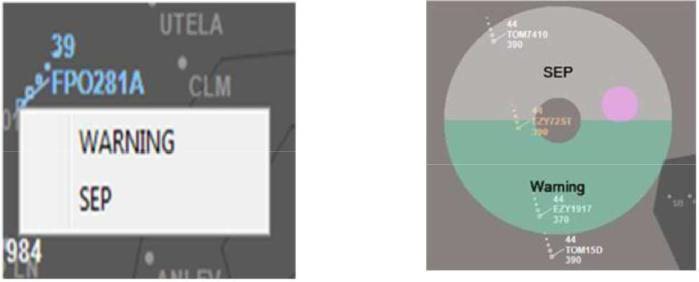
\includegraphics[width=\textwidth]{Figures/selectionFunction.png}
	\caption{
	A pulldown menu and a pie Menu.}
	\label{e:selectionFunction}
\end{figure}

\paragraph{I2-2: Pie Menu and Dwell Time}
The advantage of the pie menu is that it appears at the exact
location where the user has selected the second aircraft.
Hence, the user can directly select one of the menu items.
However, following the remarks of some users, we have
increased the delay to 500ms before opening the pie menu.
Moreover, in order to respond to the need to keep all the
parts of the radar image visible, we opted for transparent
colors (\autoref{e:selectionFunction}).

\paragraph{I2-3: Pie Menu and Gaze Gestures}
In this interaction, the user must move his or her gaze from
one of the menu items to the outside of the pie menu. This
gaze gesture launches the warning function on the selected
planes.
\subsubsection{I3: Zoom Methods}
These interactions respond to the need to freely navigate
through the radar image.
\paragraph{I3-1: Pointer centered Scroll}
This interaction exists in some ATC interfaces (mainly
interfaces without strip called "stripless"). The user acts on
the mouse wheel to zoom in or out. The zoom center is then
located at the mouse pointer. Also, it will help us to compare
the effectiveness of our new interactions.
\paragraph{I3-2: Gaze centered Scroll}
As before, this zoom technique is based on the mouse, but
this zoom is not centered on the mouse pointer anymore, but
rather on the user's gaze location on the screen. In both
techniques, the zoom returns to its original level by clicking
with the mouse wheel.
\paragraph{I3-3: Touchpad}
With the usual gestures made on a touch pad, the controllers
can perform forward zooming (Pinch open) and backward
zooming (Pinch close) centered on his / her gaze.
\paragraph{I3-4: Leap Motion}
The Leap Motion is a device that detects the movements and
aspects of the user's hands. We therefore used it to achieve
an interaction that is to approach or pull away the palm of
the hand to zoom in or out. When removing the hand form
the Leap motion's detection area , the zoom will return to
its original level.

\subsubsection{I4: Pan Methods}
Sometimes it is necessary for the controller to observe the
planes that are not necessarily displayed on the controller
screen. To do this, the user must perform lateral movements
(i.e. Pan) of the radar screen. These interactions respond to
the need to navigate through the radar image.
\paragraph{I4-1: The Mouse}
A first technique, which often exists in some air traffic
control systems, is to make lateral movements with the
mouse. The user clicks on the map then performs the
movements of "drag" to move it.
\paragraph{I4-2: Touchpad}
This technique does not use the gaze but given the presence
of the touchpad in the final prototype, we wanted to know if
the users appreciated the fact to navigate through the map
with their fingers (as we can do it in Google Map
Application for Smartphone for example).
\paragraph{I4-3: SmartPan}
Our goal was to use the eye tracker to observe directly a
calling aircraft that would be out of the controller's screen.
For this, we have designed a system with voice recognition
to detect the corresponding call sign from calling aircraft. If
the calling plane is not within the area displayed on the
screen, the system automatically displays an arrow
indicating the direction toward this aircraft. The user then
has to look at the arrow (which gets yellow thanks to the eye
tracker), and a pan is automatically processed toward the
calling aircraft. This aircraft will be displayed in a different
color for easy identification (\autoref{e:smartPan}). Once the information
is taken by the controller, he or she just need to look in the
opposite direction of the arrow and the Pan
returns to its initial value. In user testing, we simulate a
calling plane with the control software.
\begin{figure}
 \centering
	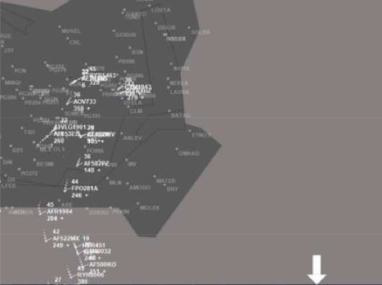
\includegraphics{Figures/smartPan.png}
	\caption{
	SmartPan: the arrow indicates a calling
aircraft outside the radar image.}
	\label{e:smartPan}
\end{figure}

\subsubsection{I5: Heat map}
The heat map is already widely used in other areas and
allows ATC to analyze the gaze of a user by recording the
history of the recorded gaze locations. These locations are
then transcribed in the form of a color gradient indicating
regions of interest on which the user focused on. When
controllers interact with each other to discuss a situation,
they often have to share information from the radar screen
and to highlight aircraft to clarify the situation. The idea
here is to use the heat map as a support to discussions and to
solve conflicting aircraft situations. When one of the
two controllers do not immediately identify the area his or
her colleague is talking about, one can press a button or a
key to display a heat map tracing the gaze history (about 20
seconds of past gazes) of the areas observed (\autoref{e:heatmap}). The
controllers can then have an overview of the specific
situation and find a solution to address it.

\begin{figure}
 \centering
	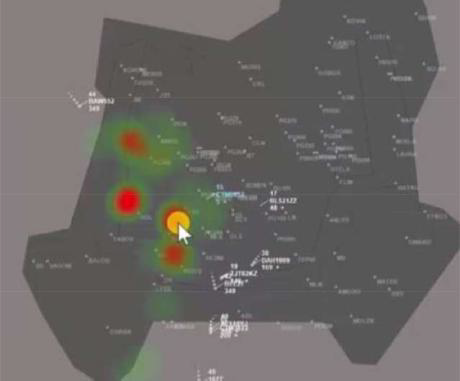
\includegraphics{Figures/heatmap.png}
	\caption{
	Heat map showing the most viewed areas +
improved magic pointer display the mouse cursor
inside the most viewed area}
	\label{e:heatmap}
\end{figure}

\subsubsection{I6: Improved Magic Pointing}
This interaction takes is root from the heat map
computation. Its goal is to display the mouse pointer at a
suitable location when the controller has to use it and thus
avoid too long mouse drag to reach the suitable pointing
target. To do so, just before the controller touch the mouse,
the algorithm computes the heat map. When the user moves
the mouse pointer, the system will display the mouse pointer
location at denser gaze location (\autoref{e:heatmap}).

\subsection{Evaluation of the prototype}
The first task was to change the state of two aircraft in a
conflict situation into "Warning". This task involved the use
of a selection method and the warning function. The second
task was to give a clearance (change of altitude or speed) to
an aircraft located in a dense traffic area. This task required
the use of a zoom technique. The third task was to give a
clearance to an aircraft located outside the area displayed on
the screen. We had the opportunity to test a method of pan.
And finally, the last task was to show the recorded gaze
location on the screen via a heat map.
Each of these tasks has been performed with each of the
proposed interactions including the techniques used in the
current ATC systems. At the end of each task, the user had
to give their opinions by filling a questionnaire asking a
qualitative evaluation of each of the interaction techniques.

The heat map was generally appreciated, especially by the
instructors. Indeed, they found that it would be very
interesting during the training courses of controllers in the
sense that this heat map would help them observe and
correct the visual path of apprentice. It is also a good help
for the other controllers who will be able to know if their
colleague is aware or not of a conflicting situation. The
zoom centered method on the gaze using the mouse wheel
was the method that received the most positive comments
from users.
Following user tests, many interactions have been improved
and new ones were created to best meet the needs of air
traffic controllers. To select an aircraft with only the eyes,
we designed another solution. When the plane is gazed, two
small labels appear on its side.

Regarding the selection of functions, the pie menu was not
easy to master, either with the selection of items via the
dwell time or worse through gaze gestures. In stressful
situations, involuntary actions could take place. To address
this, we proposed a validation of pie menu items via a button
or keyboard. We also added a visual feedback on the gazed
item in order to meet user' needs during the first test
session.
To compensate the loss of calibrations noticed during the
tests, we implemented an algorithm called Bubble Cursor  (see
\cite{Grossman:2005:BCE:1054972.1055012}). This algorithm consisting in computing the nearest
neighbor of the user gaze location. Thus, even if the eye is
not perfectly on one of the aircraft in the control area, the
nearest aircraft is still selected.
\section{Introduction}
Volumetric data found in many fields, such as engineering, material sciences, medical imaging, astrophysics. Their exploration is not trivial, and heavily impacted by the users' needs. In most airports, security agents deal with such data exploration during baggage inspections. They use two types of fluoroscopic systems: X-ray and tomography scanning systems. X-ray system provides a flattened 2D baggage scan while tomography scanning system produces transversal scans, also called slices. 
Thanks to data processing (e.g. \cite{deans2007radon}), they can produce a full 3D scan (set of voxel with their corresponding density).
Our input data is a uniformly sampled multivariate field F : D $\longrightarrow$ V, D $\subset \mathbb{R}^{n}$ 
,V $\subset \mathbb{R}^{m}$ with n = 3 (volume) and m=1 (scalar field).



\section{Activity analysis}

During this thesis, I had the opportunity to intend to training courses for security agents' instructors, and to visit an airport (Toulouse-Blagnac Airport). These helped me to study the activity of security agents and get the users' needs. The training courses lasted 3 weeks. In fact, I studied weapons and Explosives, scan analysis methods, dissimulation techniques, and fluoroscopic systems functionalities. In addition, I spent 3 days among the security agents of Brink's at Toulouse-Blagnac Airport. In this section, first I describe the security agents' task by describing their equipment, the prohibited articles, and the protocol to analyze a scan. Next, I highlight their activity issues by showing the different error types, and the dissimulation techniques.

\subsection{Task description}

The airport security agents have many roles depending on their work position. They control people (the passengers, the flight crew, and the airport personnel), and the luggage at security checkpoints. The different work positions are:
\begin{itemize}
\item The reception, where the security agents check the documents and put the hand luggage on the treadmill of the X-ray machine,
\item viewing and detection of objects and luggage through X-rays,
\item pat-down search,
\item baggage inspection.
\end{itemize}
In this study, we focus on the threat detection through X-rays.

\subsubsection{The Equipment}

In most French airport, the security agents two types of fluoroscopic system: the tomograph, and the classic system. The classic fluoroscopic system provides a 2D scan of luggage on the one hand, and on the other, the tomograph can produce transversal scans in addition to the 2D scan. Some scanners are able to detect explosive automatically, they are called EDS (Explosive Detection System). The architecture of the classic system is composed of:
\begin{itemize}
\item a mechanical set comprising a frame, a conveyor, and a collimator,
\item a physical set comprising an x-ray generator, a detector, and detection cells,
\item the central unit,
\item and input/output devices (keyboard, screens).
\end{itemize}
When a luggage get in the frame, the x-rays are sent from the generator to the L-shaped detector through the luggage's components. The x-rays are attenuated depending on the molecular density of the encountered objects, which allows to receive different x-ray intensities on the L-shaped detector. Then, the different received intensities are processed to get the final 2D scan.
The final image does not keep the original colors, instead they use 3 colors (orange, green, and blue) to show the density of each encountered object. The orange color is used for low density matters which are mainly organic. In opposition, the blue color is used for high density matters which are mainly inorganic. The green color expresses the superposition of different kinds of materials or average density materials, see \autoref{f:image2d}.

\begin{figure}
\centering
	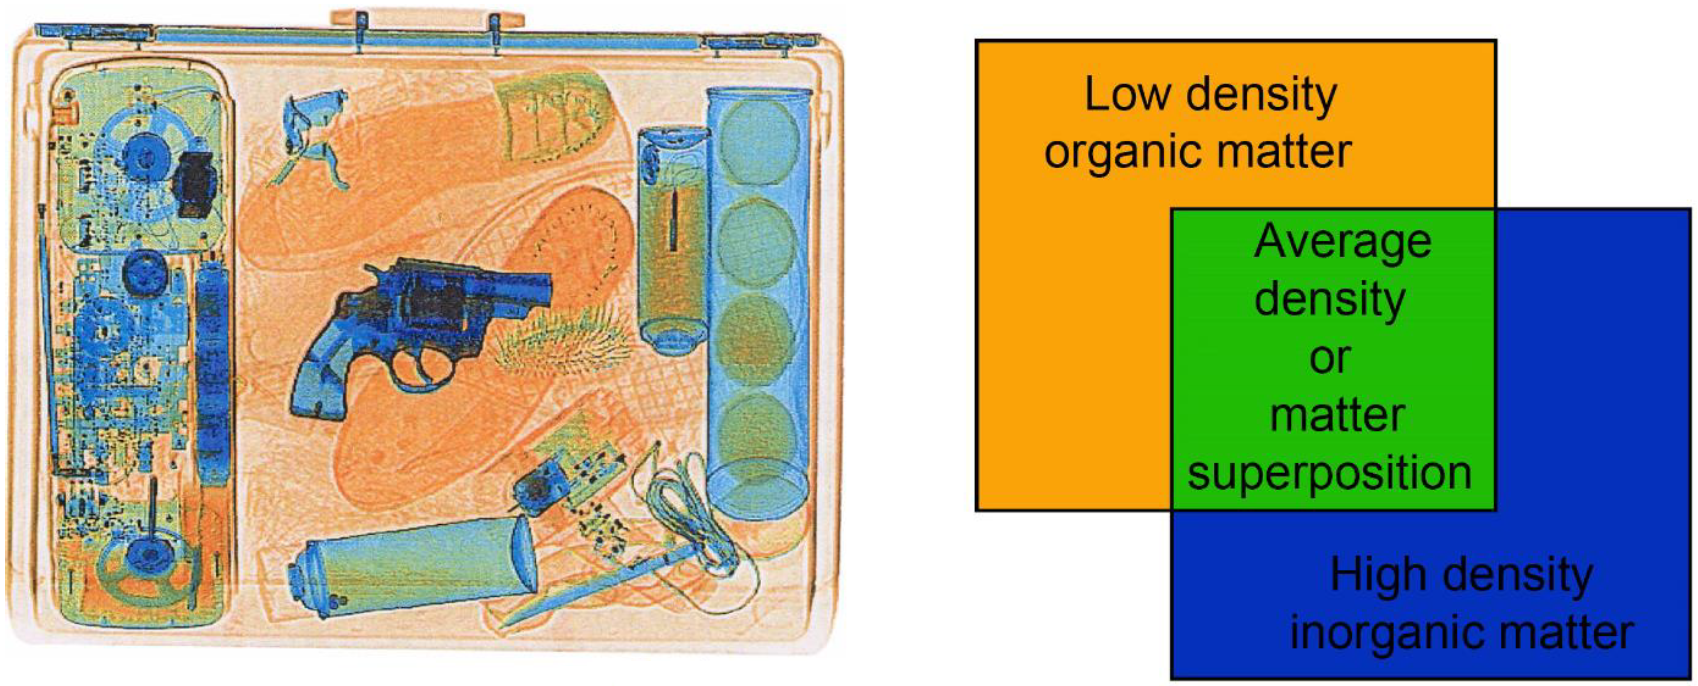
\includegraphics[height=5.2cm]{Figures/contour}
	\caption{ X-ray scan with the 3 standard colors (orange, green, and blue)}
	\label{f:image2d}
\end{figure}

\subsubsection{Prohibited articles}
Depending on the context, there are many prohibited articles. The aim is to avoid any kind of weapon to board in the aircraft. According to the regulations, weapons are items intended primarily to kill, injure, immobilize or reduce to impotence. The prohibited articles are:
\begin{itemize}
\item Guns, firearms, and any other equipment emitting projectiles,
\item Stun devices,
\item objects with a sharp tip or a cutting edge,
\item working tools,
\item blunt instruments,
\item explosive or incendiary substances and devices.
\end{itemize}
In addition to these prohibitions, some articles such as liquid, gels, and aerosols are restricted.

\subsubsection{Scan analysis}
Whatever fluoroscopic system is used, the security agents try to follow an analysis protocol to ensure any prohibited article is detected. This protocol is composed of 4 major steps, which are the global picture analysis, the in-depth analysis, the structure analysis, and the context.

\paragraph{Global picture analysis}


First, the security agent check whether the luggage is well placed. Indeed, the luggage should appear on the screen with \ang{45} of rotation. If it is not the case, a re-positioning is required. To avoid this issue, another agent must check the luggage positioning.
Next, the agent try to find out whether the luggage is complex or not. A luggage is complex when there is a superposition of usual objects and metallic materials. A complex luggage can hide threat and make them invisible. If possible, the complex luggage is opened and all troublesome objects are removed.

\paragraph{The in-depth analysis}


First, the security agent divides the luggage's component in groups. The aim is to reduce the risk of error. Indeed, smaller prohibited articles may be easily unseen. Then, the dark areas must be lightened up. To do it, the security agent can use functionalities such as high penetration or contour enhancement. If the area is still dark, the luggage must be opened to remove the serious doubts.
Next, the agent focus on the problematical shapes. A non-recognizable shape may be caused by a bad positioning. Any unrecognized object must be inspected by the agent. If any prohibited article is detected, the agent follows the procedure related to the threat. In addition, an organic matter superposed to an electronic device is considered as a sufficient reason to open the luggage. Liquids, gels, and aerosols should be less than 100ml otherwise they will be removed from the luggage. These liquids should be placed into a plastic bag.

\paragraph{The structure analysis}


During this step, the security agent compare each element of the luggage which must be symmetrical because of its industrial conception such us suitcase's wheels. If the symmetry is not respected, it is might be a clue to the deliberate luggage modification for dissimulating prohibited objects.

\paragraph{The context}


Depending on the context some articles are prohibited or not. The agent must be aware of his work position.
On an explosive detection system, the threats are already highlighted. The agent's job is to verify whether the threats are real or not.
In our study, we focus on a conventional system to provide new interaction techniques for analyzing 3D luggage scans.

\subsection{The activity issues}
There is many level of security in luggage inspection depending on the airport (between 1 and 6). Humans and machines work together to detect any potential threat inside the luggage. At the lowest levels of security, the security agents are in contact with the passengers, and therefore face 4 main operational constraints for safety and economical reasons: Facilitation, security, speed, and self-protection. 

First of all, The facilitation constraint implies that the security agent has to ensure a good user experience to the customers (the passengers). Second, they must prevent any potential threat to pass their inspection. In addition, they have to protect themselves from different kind of threats (ill-intentioned persons, parcel bomb). And finally, economical reasons oblige them to be fast enough in order to ensure a good flow. Therefore, the security agent face a trade-off between these four constraints, see  \autoref{f:constraints} .
\begin{figure}
\centering
	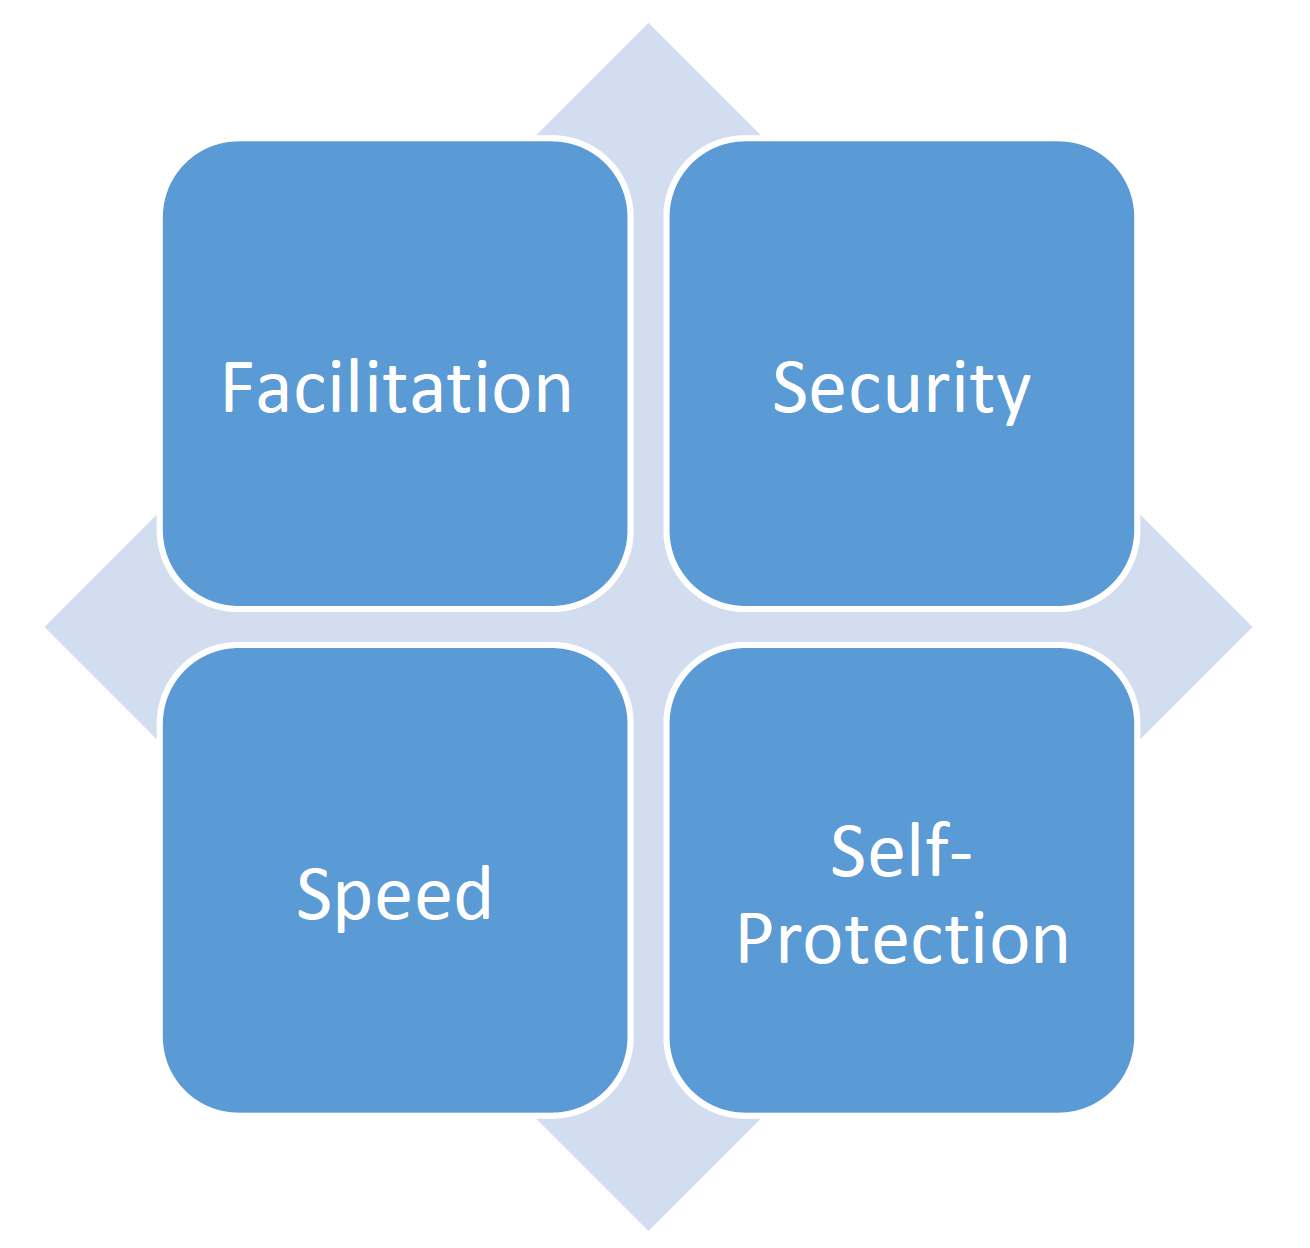
\includegraphics[height=5.2cm]{Figures/constraints}
	\caption{The operational constraints of the security agents.}
	\label{f:constraints}
\end{figure}



\subsubsection{ Error Types }


The security agents can usually do 3 types of error during the baggage inspection process.

\paragraph{Perception errors}

The security agent does not detect the right area to analyze. He is not focus on the troublesome area, see  \autoref{f:perception}.
\begin{figure}
\centering
	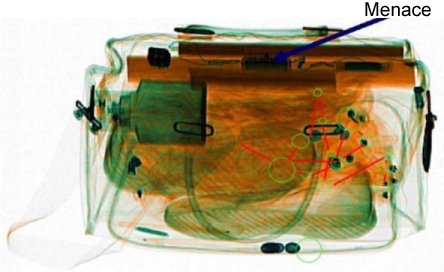
\includegraphics[height=8cm]{Figures/perceptionError}
	\caption{Perception error. The security agent do not notice the menace at the top of the image (the initiating system of an explosive) }
	\label{f:perception}
\end{figure}
\paragraph{Interpretation errors}

The security agent detects the right troublesome area but does not judge it as a potential threat. In other words, he is focused on the right area but cannot see the menace. The agents used to combine what they find out with their knowledge on real world objects stored in their memories. They have their own model of the situation, see  \autoref{f:interpretation}.
\begin{figure}
\centering
	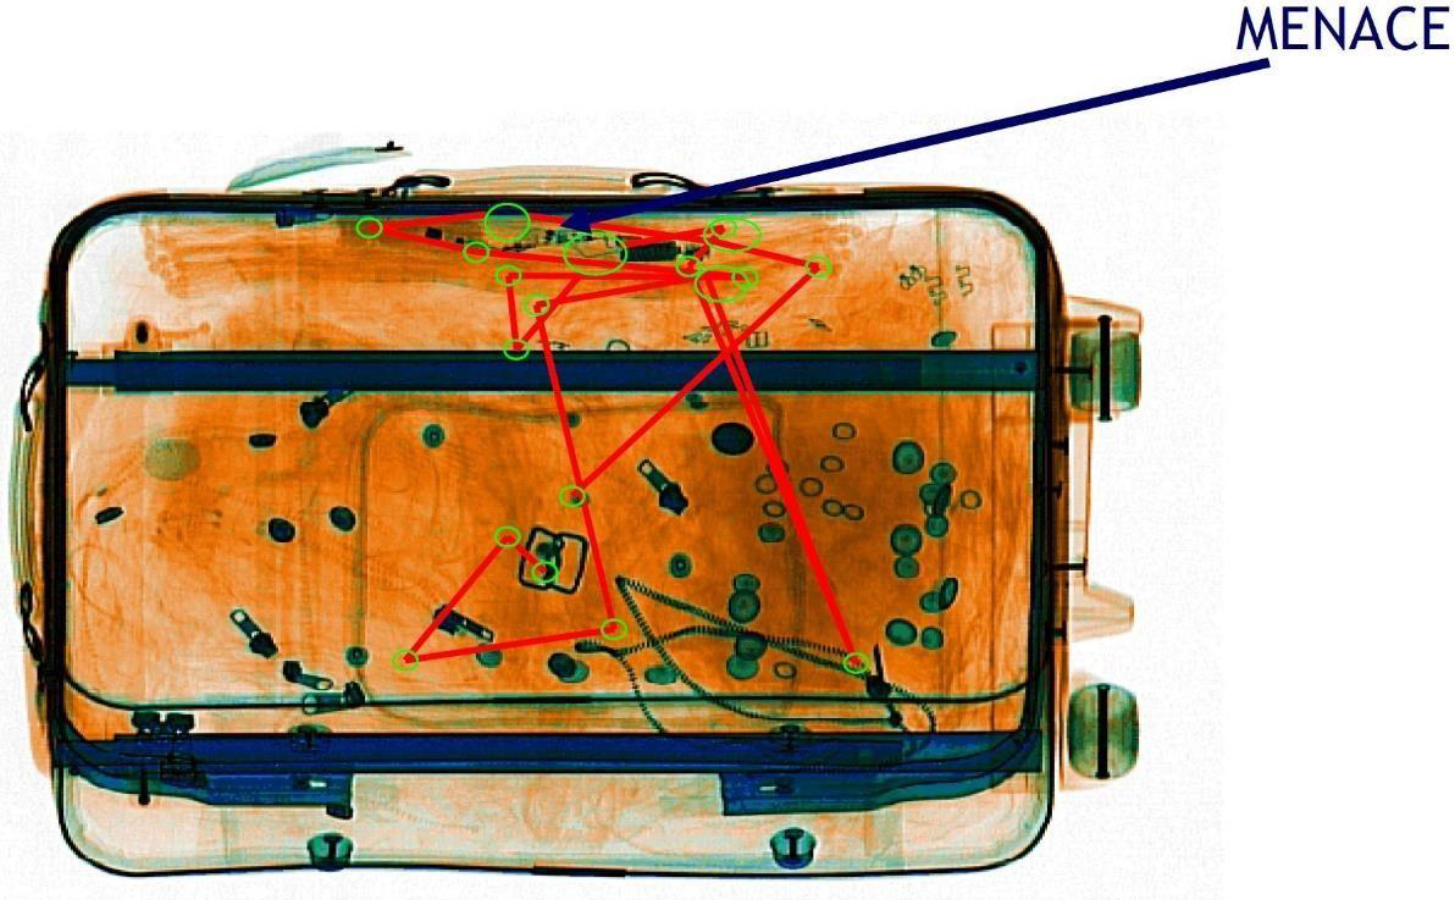
\includegraphics[height=8cm]{Figures/interpretationError}
	\caption{Interpretation errors. The security agent notice the menace at the top of the image do not interpret it as a threat (the initiating system of an explosive)}
	\label{f:interpretation}
\end{figure}

\paragraph{Decision making errors}
In this case, the security agent detects the right troublesome area with a good interpretation, but make a bad decision. It might be related to the context or the procedure knowledge.
In addition to these errors related to the agent, four hiding techniques can be used to bypass the security mechanisms. Those techniques are superposition, positioning, dissociation, and bait.

\subsubsection{ Dissimulation techniques }
Since the resulting X-ray scanned image only contains densities, it cannot display the material original colors. The standard color visual mapping uses 3 different colors (orange, green, and blue) to display the data density. Orange color corresponds to low density (mainly organic items). In opposition, blue color is used for high density items (e.g. metal). In the case of X-ray systems, green color corresponds to the superposition of different kinds of materials or average density materials (\autoref{f:image2d}). 

The displayed 2D scanned image can suffer from four issues.

\textbf{Superposition}: A threat (e.g. prohibited object like knife, cutter…) may be sheltered behind dense materials. Sometimes, it is possible to see through these blind shield using some functionalities such as high penetration (enhanced X-ray power) or image processing (contrast improvement),  see  \autoref{f:superposition}. 
\begin{figure}
\centering
	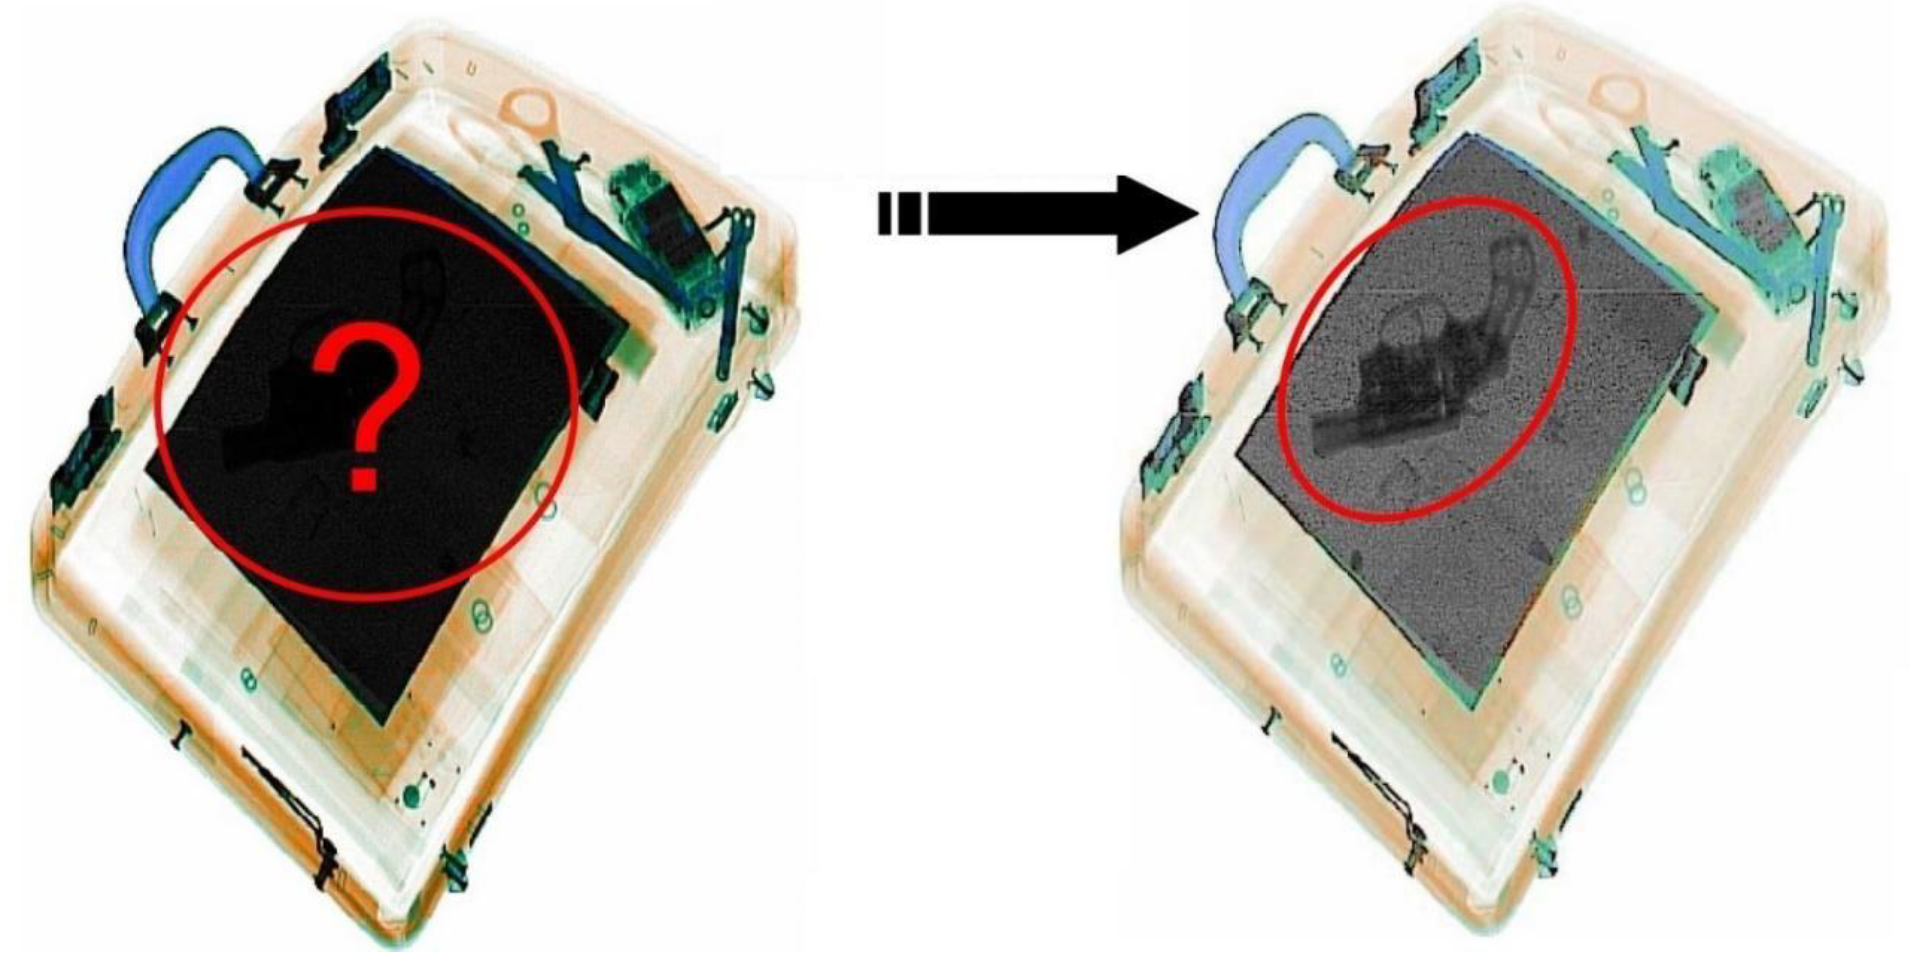
\includegraphics[width=0.95\textwidth]{Figures/superposition}
	\caption{Dissimulation by superposition}
	\label{f:superposition}
\end{figure}

\textbf{Location}: Depending on its location inside the luggage, a threat can be difficult to detect. Objects located in the corners, in the edges or inside the luggage's frame are very difficult to identify,  see  \autoref{f:location}.
\begin{figure}
\centering
	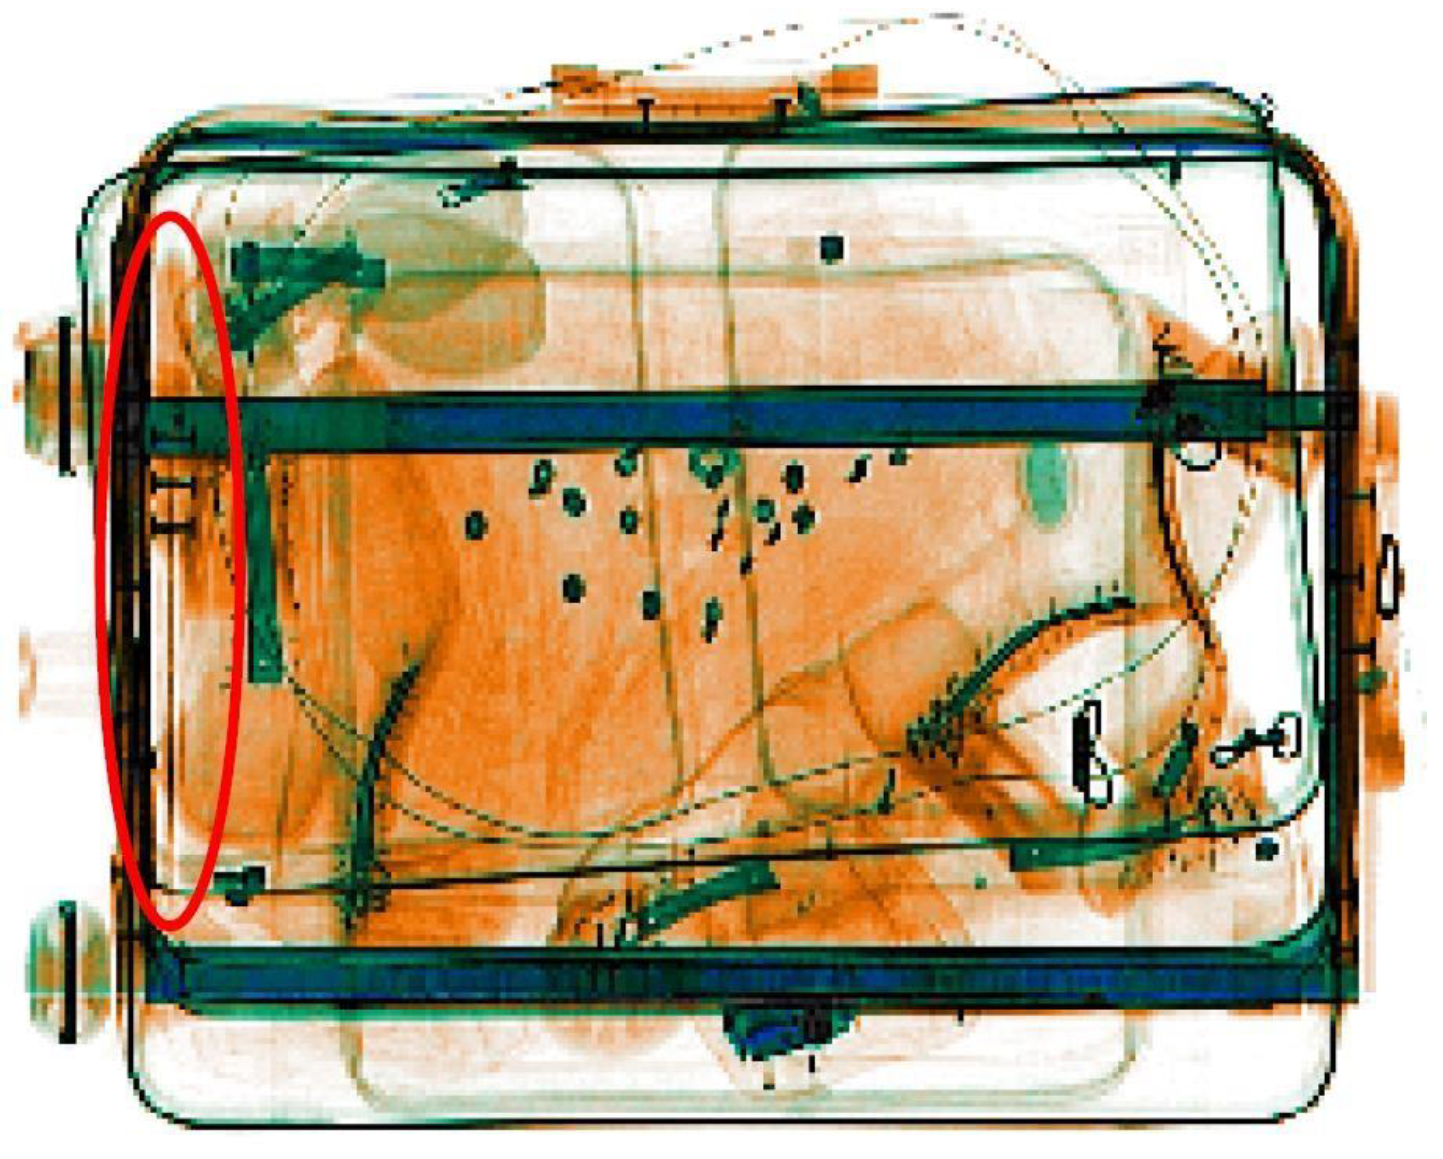
\includegraphics[width=0.9\textwidth]{Figures/positioning}
	\caption{Dissimulation by the location}
	\label{f:location}
\end{figure}

\textbf{Dissociation}: Another way to dissimulate a threat is to separate and to spread parts of it in the luggage (weapon or explosive are composed of many separated items like the trigger, the cannon...). This dissociation can be combined with other dissimulation techniques,  see  \autoref{f:dissociation}.
\begin{figure}
\centering
	\includegraphics[width=0.8\textwidth]{Figures/Dissociation}
	\caption{Dissimulation by dissociation}
	\label{f:dissociation}
\end{figure}

\textbf{Lure}: An ill-intentioned individual may use a lure to hide the real threat. For instance, a minor threat like a small scissors may be clearly visible and catch security agent's attention while a more important threat remains hidden, see  \autoref{f:bait}.
\begin{figure}
\centering
	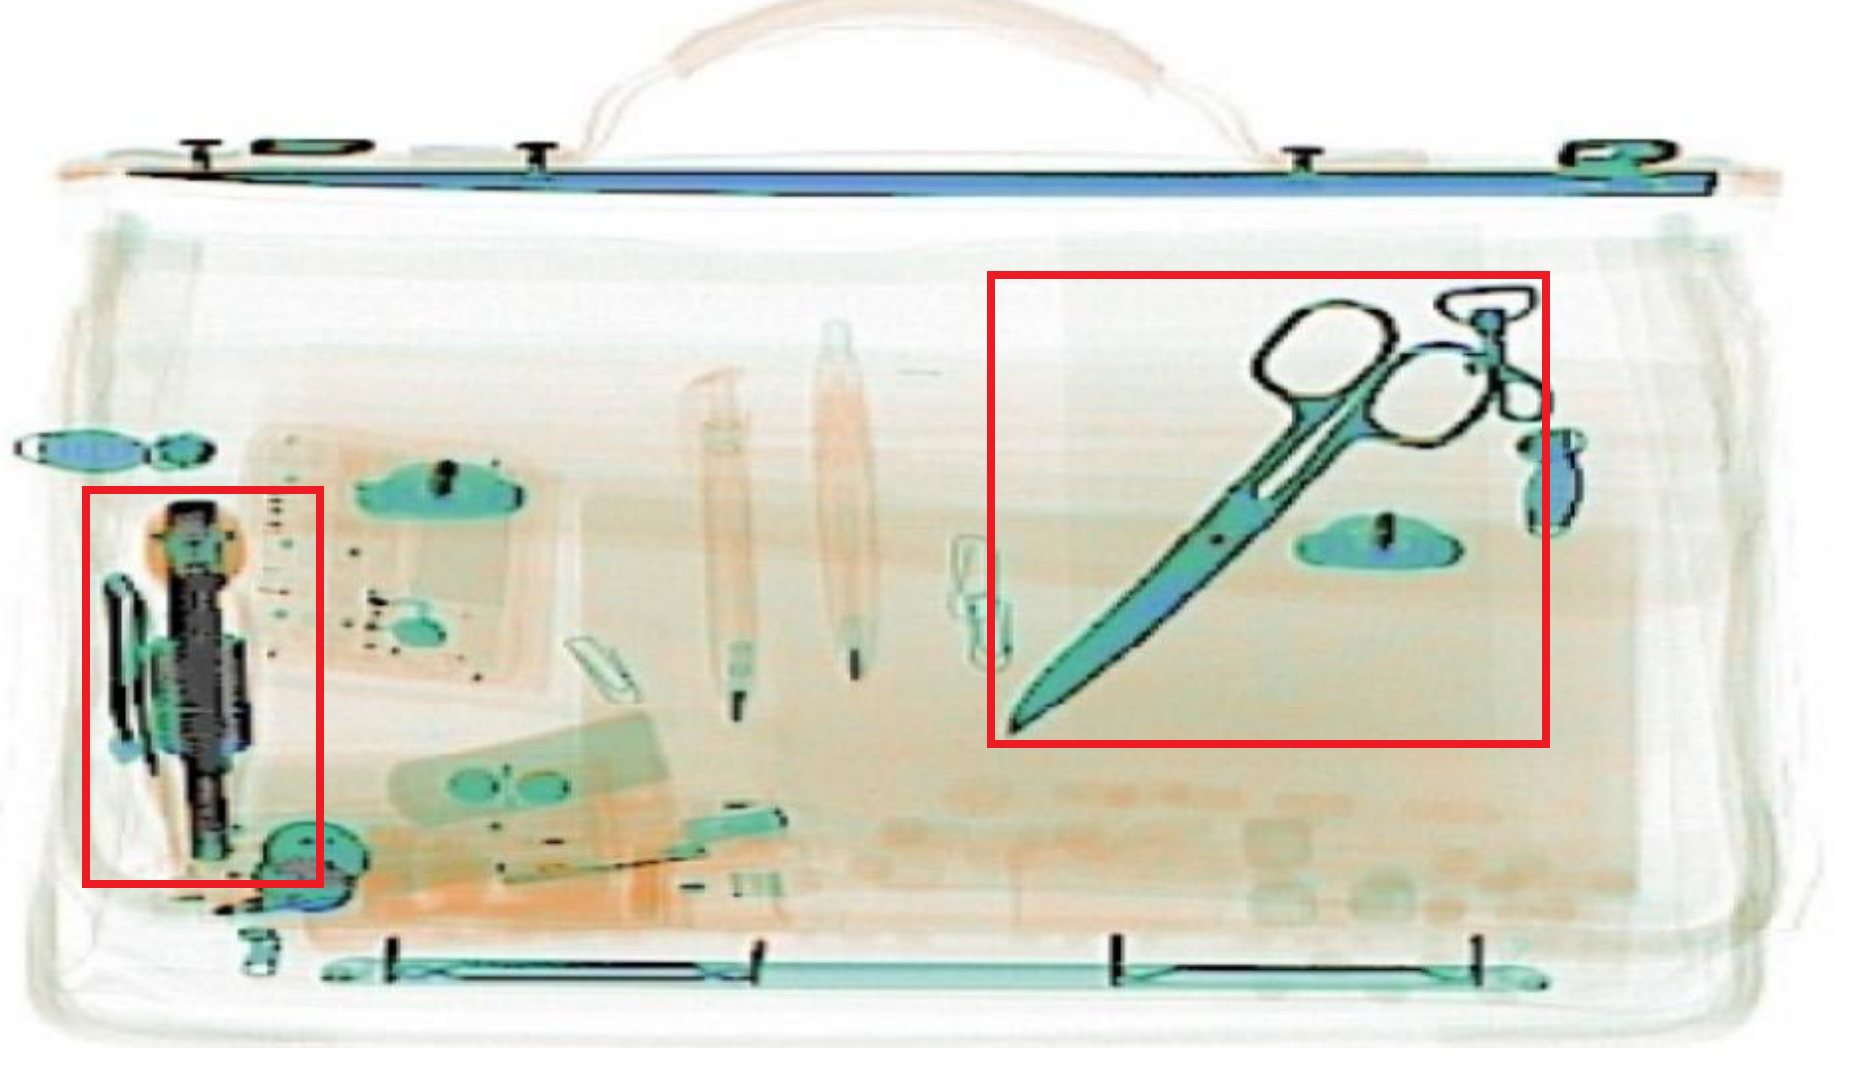
\includegraphics[height=8cm]{Figures/bait}
	\caption{Dissimulation using a bait}
	\label{f:bait}
\end{figure}

\subsection{ Requirements }


3D baggage scan exploration are one potential solution of such limitations, but to the best of our knowledge no previous existing system investigated this activity domain with interactive volumetric exploration tools. Even if extensive works have been done in medical 3D scan exploration and manipulation ~\cite{preim2013visual}, there is a great opportunity to adapt and develop new interaction and data manipulation techniques to support 3D baggage exploration.

We performed on site observations with contextual inquiry (one day observation in one of the major French airport). We also conducted one brainstorming with four security practitioners from which we defined relevant use cases. Thanks to these analysis, we extracted a set of top level needs and requirements :

•	VIS: users need to visualize the content of the luggage.

•	EXP: users have to explore the baggage with interactive navigation system.

•	OCL: the system must provide tools to address occlusion issues; the
superposition of items inside the luggage hinders their visualization.

•	INT: User need to explore luggage with simple interactions. User knowledge is too limited regarding volumetric data processing to understand the involved techniques and their parameters.

\section{ Interactive exploration of 3D scanned baggage }

\subsection{Top Level Structure}

Our system is composed of one main view (Volume Visualization) and 5 sub views to control and customize it, see  \autoref{f:layout}. Our interactive system does not provide menu and every feature is directly accessible from this main view (\autoref{f:layout}).
The Volume Visualization can contain up to two views to ease interactions with the 3D scan. These views display the baggage and one can navigate through it (zoom, pan, rotation), manipulate its content (brushing, selection, deletion). These two views can be linked or disconnected in order to inspect selected objects with or without their context.
A smaller view called Overview shows the location of the investigated area. The overview is one-eighth the size of the main window and is located at its bottom right.
\begin{figure}
\centering
	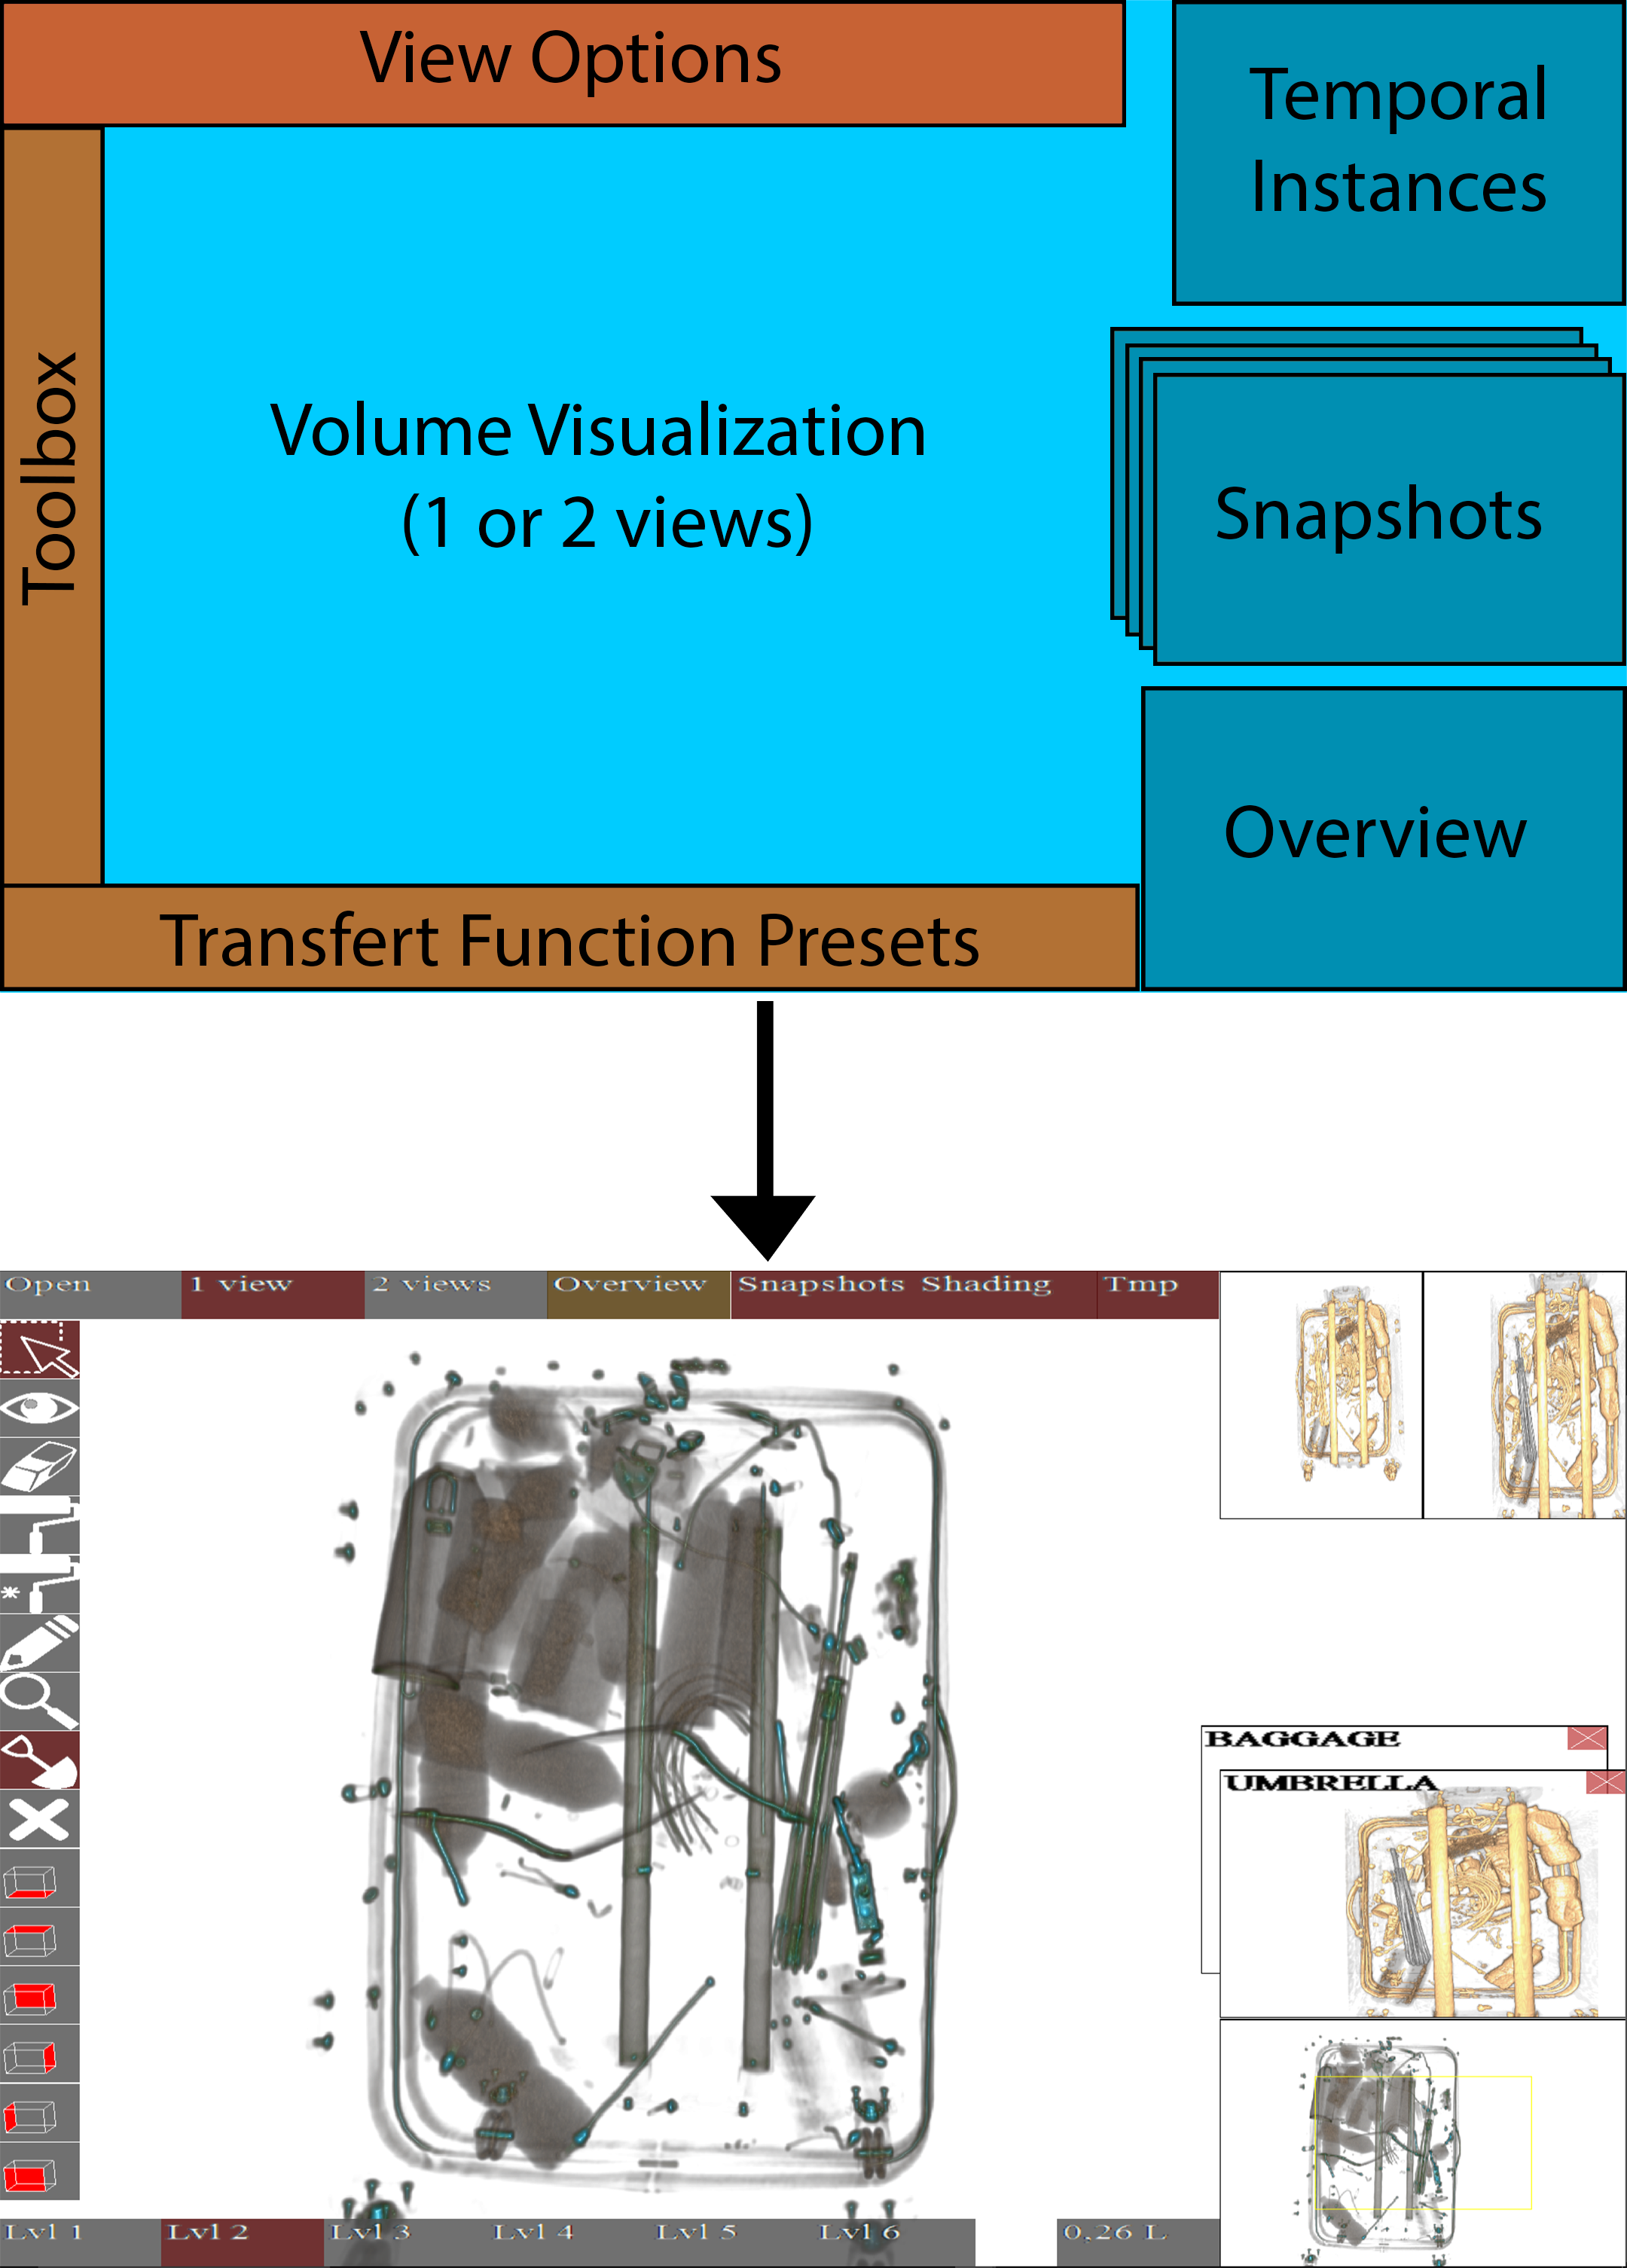
\includegraphics[height=14cm]{Figures/layout}
	\caption{Top level layout and screenshot of our Graphical User Interface. All the features are available through this GUI}
	\label{f:layout}
\end{figure}

Temporal Instances window, located in the top right of the interface, shows the current and the previous settings of the Volume Visualization. The current setting is modified when the user changes the transfer function or manipulates an object.
The Snapshot shows saved instances with their setting (pan, zoom, rotation, transfer function, selection, brushing).
The Toolbox contains every interactive tools to explore the baggage (brushing, selection, eraser, density picker, navigation tools).
Transfer Function presets contains six predefined settings ordered by their filtering power. Low level shows every density, high level only show high density values. 

This global layout can be customized thanks to View Options. One can display one or two views of the Volume Visualization, the Temporal Instances, the Snapshot and the Overview.

\subsection{Interaction techniques}

We used a multi touchscreen Wacom 24HD equipped with a stylus. Most of the developed interactions can be performed with every available modality: mouse, hand or pen.
\subsubsection{ Transfer function edition}	
Datasets such as two dimensional raster images or three dimensional voxel based representations are often processed for representation using a transfer function (TF) defined by a curve. 

Since airport security agents have a reduced time frame and limited knowledge of technical constraints, we defined six TF presets (\autoref{f:preset}). These presets only modify the TF transparency curve while keeping the same color mapping. These presets are ordered by their density filtering power: the first preset displays every density and the last one only highest density of the volume (i.e. metal). 

\begin{figure}
   \centering   
	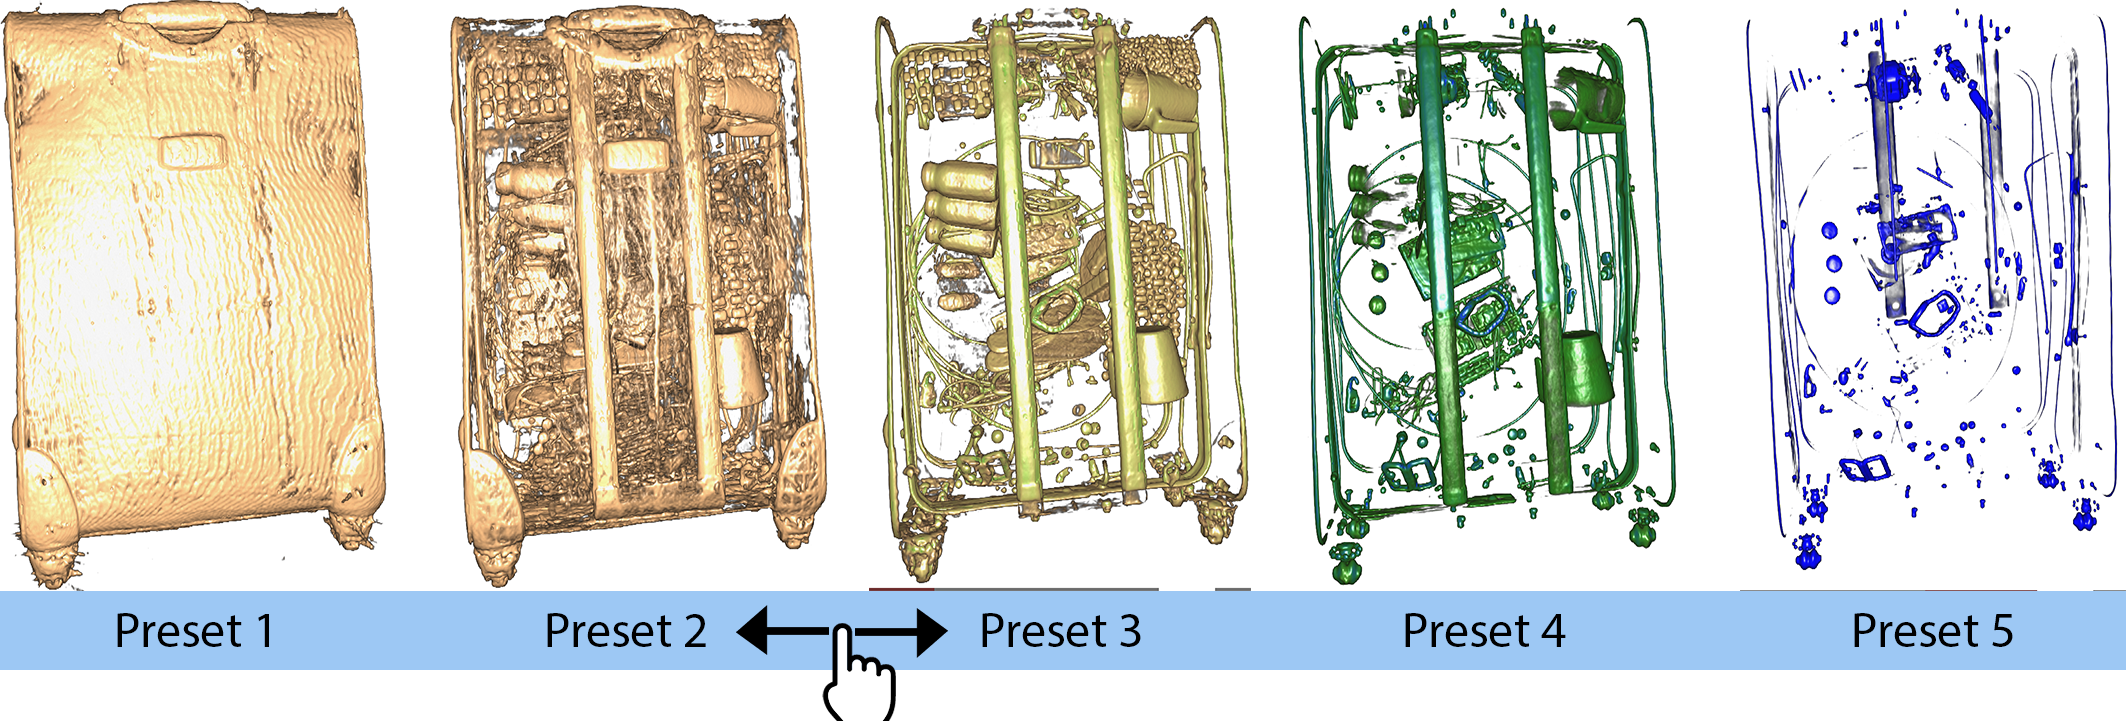
\includegraphics[width=15cm]{Figures/preset.png}
	\caption{ Transfer function presets and their continuous interaction. The high density materials are revealed by dragging from left to right on the presets }
	\label{f:preset}
\end{figure}
When clicking on a preset, the TF changes with a short transition (1 second) toward a new one. 
Finally, the user can select a transfer function located between two presets. To do so, the user drags from any location within the TF presets area until the volume visualization shows interesting features 

\subsubsection{ Objects selection and investigation}
In order to investigate in detail a specific object, one can isolate it, remove surrounding items to address occlusion issues, or find a suitable point of view (\autoref{f:menace}). This section details these interaction techniques which encompass the selection of  many objects.


\paragraph{	Selection of an object}
We developed three different ways to select objects with the three different modalities: hand, mouse or pen. When using his or her hand, the user has to double tap the desired object with his or her finger. When using the pen, the user must press the biggest button on the stylus while pointing at the target. Otherwise, the user has to double click on the target with the mouse pointer. After the target is selected, our system tries to find a better point of view to display the selected object with the minimum of occluded parts. The details of this algorithm will be explained in the technical part of this study. We use a smooth transition to rotate and zoom the baggage. 


\begin{figure}
\centering   
	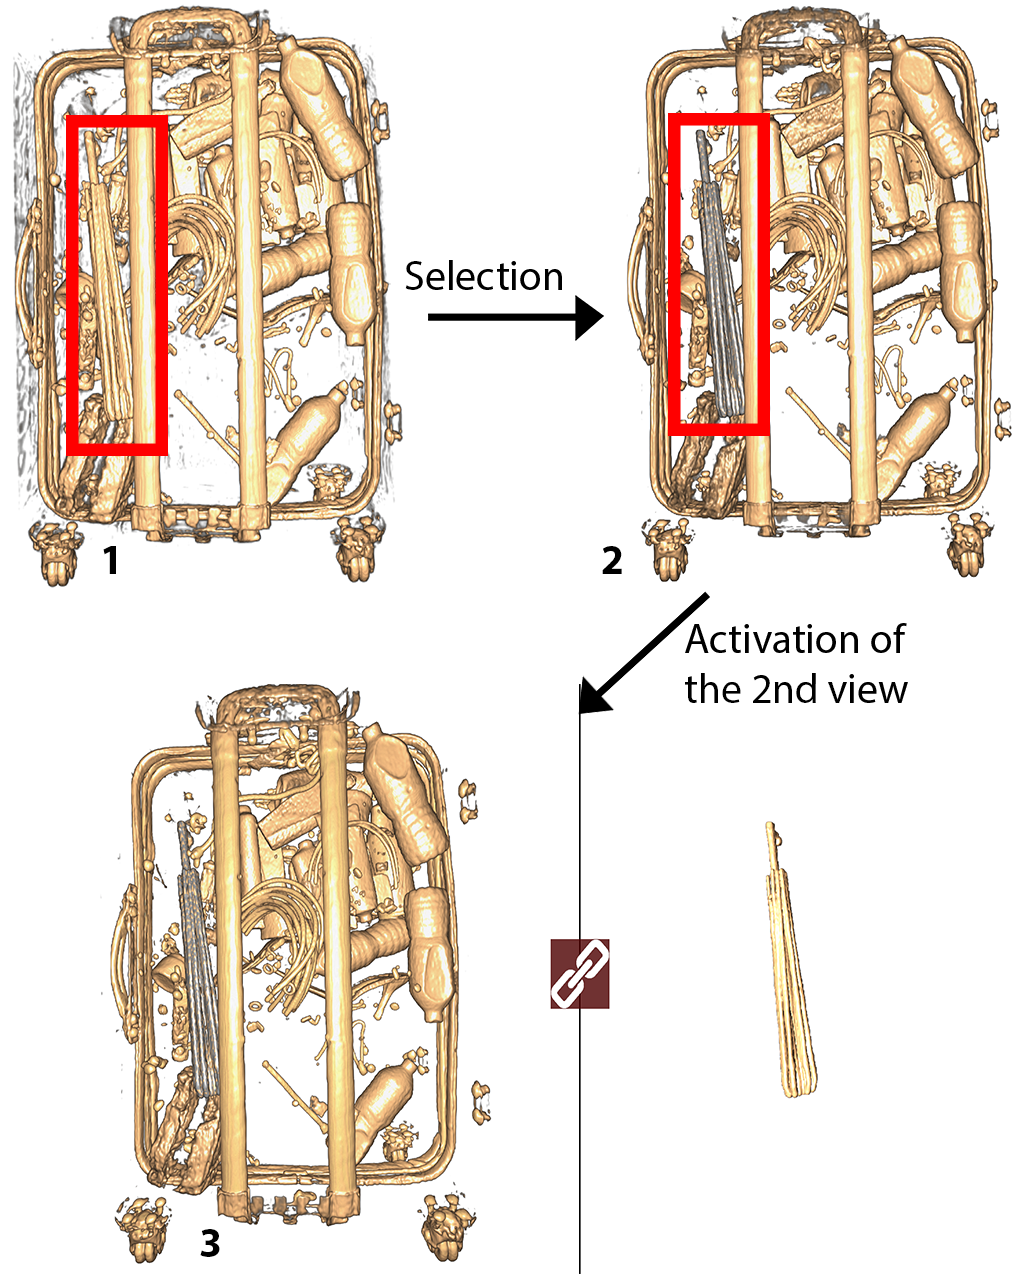
\includegraphics[width=9cm]{Figures/selection.png}
	\caption[Selection of an umbrella for further inspection.]{ Selection of an umbrella for further inspection.  1- The user wants to check an object looking like an umbrella. 2- After a double click, the object is selected and becomes gray as a feedback. 3- After the activation of the 2nd view, the user can manipulate the umbrella with or without the whole baggage. All the Selected items are also available on this second view. }
	\label{f:selection}
\end{figure}



If the user has activated the 2 views Volume Visualization (Button 2 views in the View Option panel), the selected object is isolated in the second view (on the right side of the main view \autoref{f:selection} ). The selection is incremental and many object can be selected one after another. To undo the selection, the user has to select the desired object in the second view.

\paragraph{Occlusion management}

In order to address occlusion issues, the eraser tool can interactively remove selected objects from one view to the other one. This interaction is similar to the selection interaction with all the modalities (mouse, hand, and pen). When using his or her hand, the user has to double tap the desired object with his or her finger. When using the pen, the user must press the biggest button on the stylus while pointing at the target. The user can also double click on the target with the mouse pointer. To restore a deleted object from one view, the user has to erase it from the other view. This simple principle guarantees that every item of the baggage is always visible while addressing occlusion issues (\autoref{f:deletion}).

\begin{figure}
\centering   	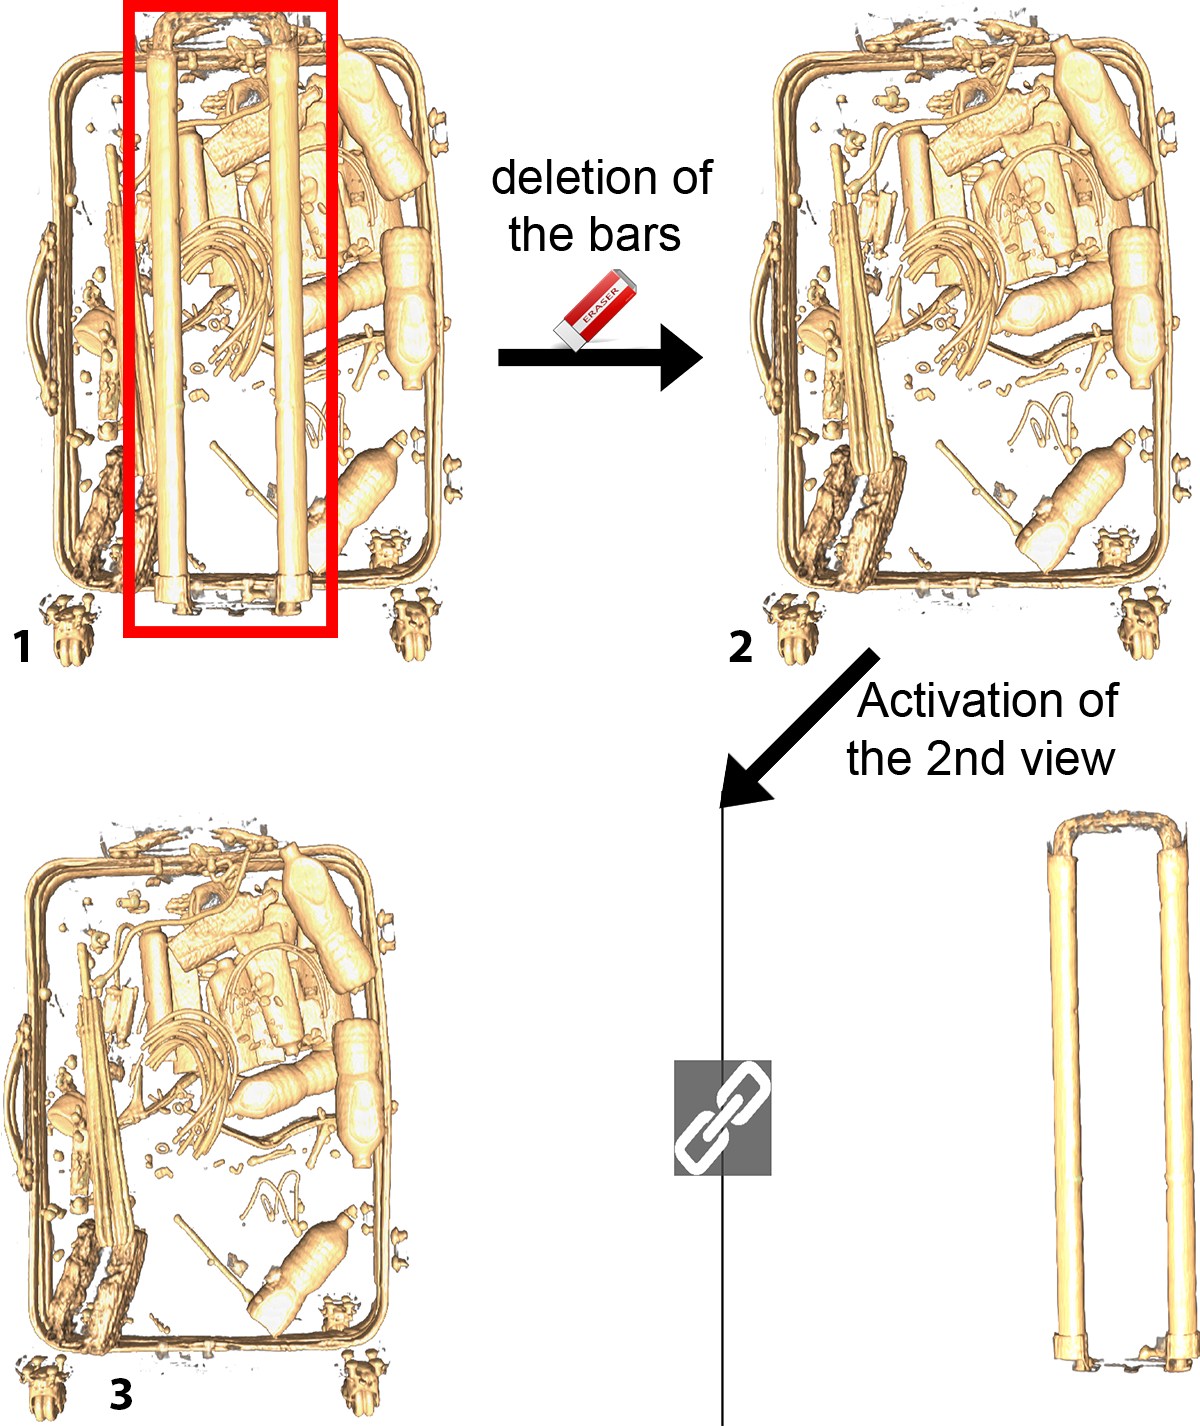
\includegraphics[width=9cm]{Figures/deletion.png}
	\caption[ Addressing occlusion issue by removing objects from one view to another one.]{ Addressing occlusion issue by removing objects from one view to another one. 1- The user wants to remove the bars of the baggage. 2- After a double click with the deletion tool, the object is removed from the main view. 3- After the activation of the 2nd view, the removed objects are visible outside the baggage.}
	\label{f:deletion}
\end{figure}

\subsubsection{Extended Brushing techniques}

\begin{figure}
\centering   	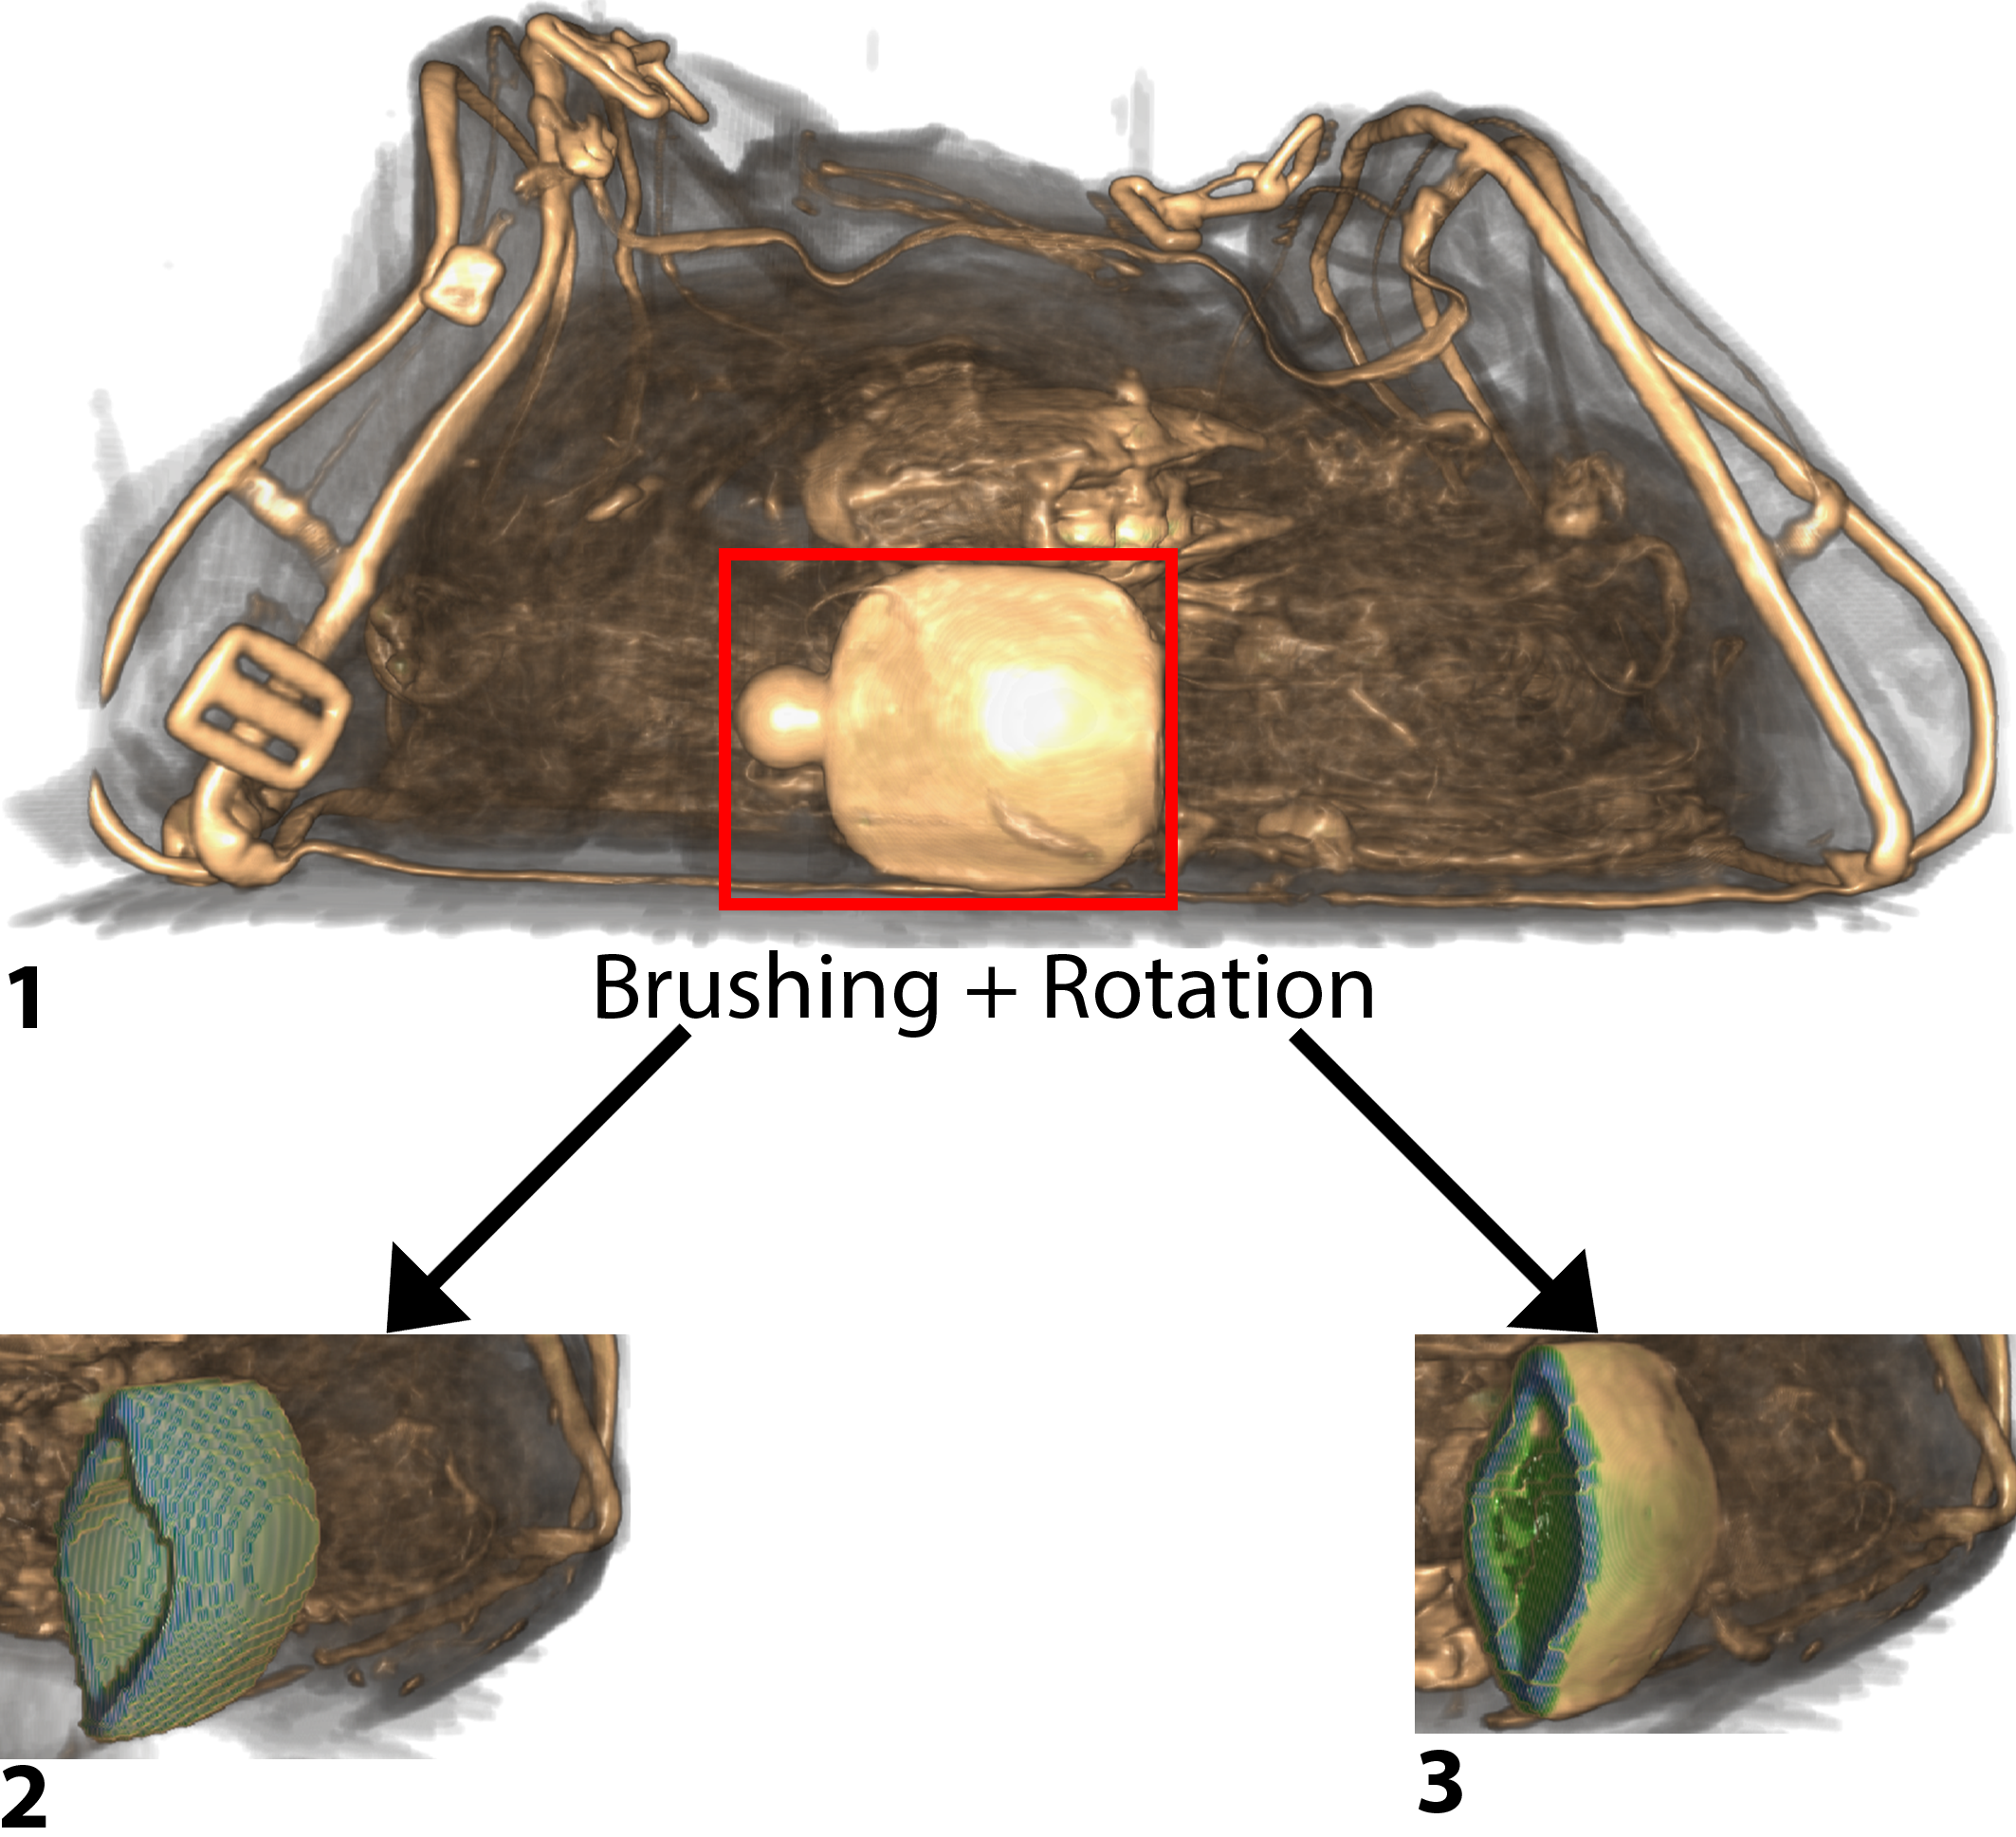
\includegraphics[width=9cm]{Figures/brushing-new.png}
	\caption[Brushing a bottle to see its content.]{ Brushing a bottle to see its content.  1- The initial baggage before brushing. 2- The result after using the old brushing technique: the content of the bottle has been removed too. 3- The result after using the new brushing technique: the content of the bottle is still visible. This brushing technique removes until it encounters an object out of the selected density range. }
	\label{f:brushing_new}
\end{figure}

Baggage is composed of low density items (e.g. fabrics, clothes, papers, organic objects…) and high density ones (e.g. metal, electronic components…). Low density items are more numerous and surround high density ones. In order to perceive a metallic object, one needs to remove or hide its surrounding low density items thanks to an adequate TF. Since TF is applicable to the whole volume visualization, the visualization of a metallic bottle will prevent to visualize its content (i.e. organic density). One cannot find out whether the metallic bottle is empty or not (\autoref{f:brushing_new}). To solve this problem, we developed two brushing techniques to explore the baggage by the mean of local removal of specific densities without modifying the TF.

\paragraph{Range Based brushing technique}

This interaction removes all voxels which are bounded in a user defined range. A range-slider is available on top of the transfer function (\autoref{f:brushing_range}). The user enables the brush tool in the toolbox by clicking on it and then the right button of the mouse removes the voxels beneath the mouse pointer.
Original brushing technique removes every voxel which is bounded in a density range and which is beneath the mouse pointer. In case of the exploration of a metallic bottle full of liquid, original brushing technique will remove the surrounding of the bottle as well as its content. To address this issue we developed a new brushing technique as if one digs into a baggage. This digging process will stop when a dense layer is encountered. This dense layer (e.g. the outer layer of a metallic bottle) will act as a shield to protect voxels located behind it (\autoref{f:brushing_new}).

 \begin{figure}
\centering	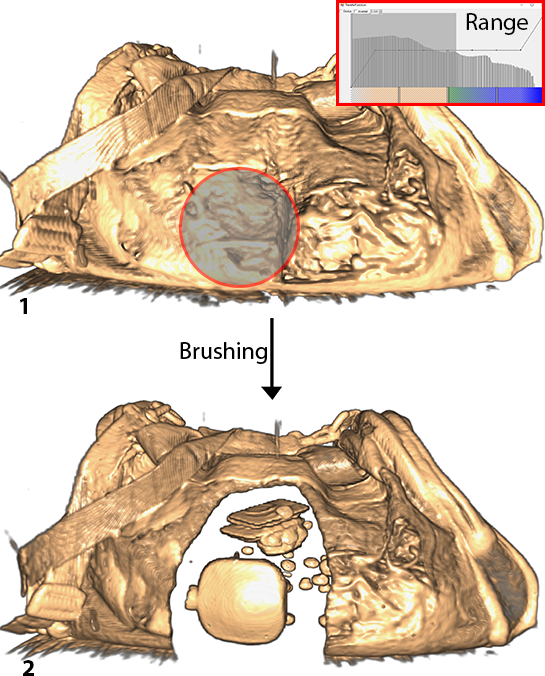
\includegraphics[width=9cm]{Figures/brushing-range.png}
	\caption[Brushing low density materials to see a metallic object hidden inside the baggage.]{ Brushing low density materials to see a metallic object hidden inside the baggage. 1- The baggage before brushing. 2- After a density range is defined, the users brushes a part of the baggage. This interaction reveals a metallic bottle.   }
	\label{f:brushing_range}
\end{figure}

\paragraph{Magic brushing technique}
This brushing technique has almost the same behavior as the range based brushing one. The main difference consist in the automatic range definition. This magic brushing removes all voxels with a lower density than the first one encountered at the beginning of the brushing process. This technique helps the user to directly define the densities he or she wants to brush. This technique avoid multiple interactions with the histogram and its range slider to define the range of brushable densities.

\paragraph{The cancellation of the brushing}
Our system offers the possibility to restore previously brushed areas. To do so, the user must select the brushing tool in the toolbox and hold the shift key while brushing over a given area. The restored densities are those defined by the histogram range slider. This restoring processing does not act as the range brushing technique and the sheltering effect (dense layer provides to brush behind it). Every voxels within the range are restored in order not to confuse the user.

\subsubsection{Snapshots}
Our system can store visual configurations thanks to snapshots. These snapshots are displayed on the right of the main view and record the current rotation, the zoom, the pan and the current transfer function.
To take a snapshot, the user must press the space bar. A name can be given to any snapshot using the keyboard. This name is displayed on the top left of its thumbnail. The user can restore a saved object by clicking on its snapshot. When a snapshot is selected, the system animates the view from its current state to the selected snapshot (pan, zoom and transfer function linear interpolation). A snapshot can be deleted by clicking on the close icon located on its top right (\autoref{f:snapshots}).
 \begin{figure}
 \centering
	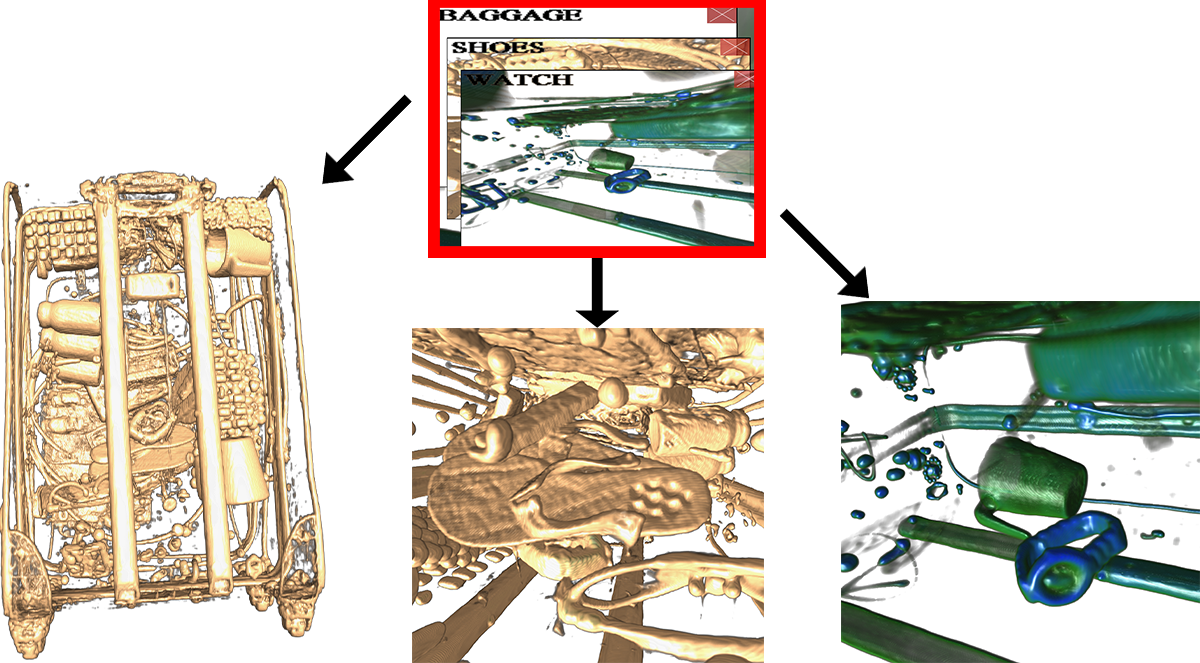
\includegraphics[width=9cm]{Figures/snapshots.png}
	\caption{ The labelled snapshots taken by the user representing objects of interest}
	\label{f:snapshots}
\end{figure}

\subsubsection{Dual temporal instance navigation}

Our system provides many animated transitions when the user explores the baggage (change of point of view, transfer function modification, item selection...) like \cite{tversky_animation:_2002}. To ease user's navigation, we added two temporal instances representing the states before and after an automatic modification of the visual configuration. This interaction is based on the undo-redo paradigm. On the top right of the main window, we added two views representing the previous state before the transition and the final one after the transition. One can navigate through this transition by dragging from one state toward the other one. The more the cursor gets close to the center of a state, the more the current view gets close to its configuration. The user can also click on the desired state to directly assign its visual configuration (\autoref{f:temporal}).
 \begin{figure}
 \centering
	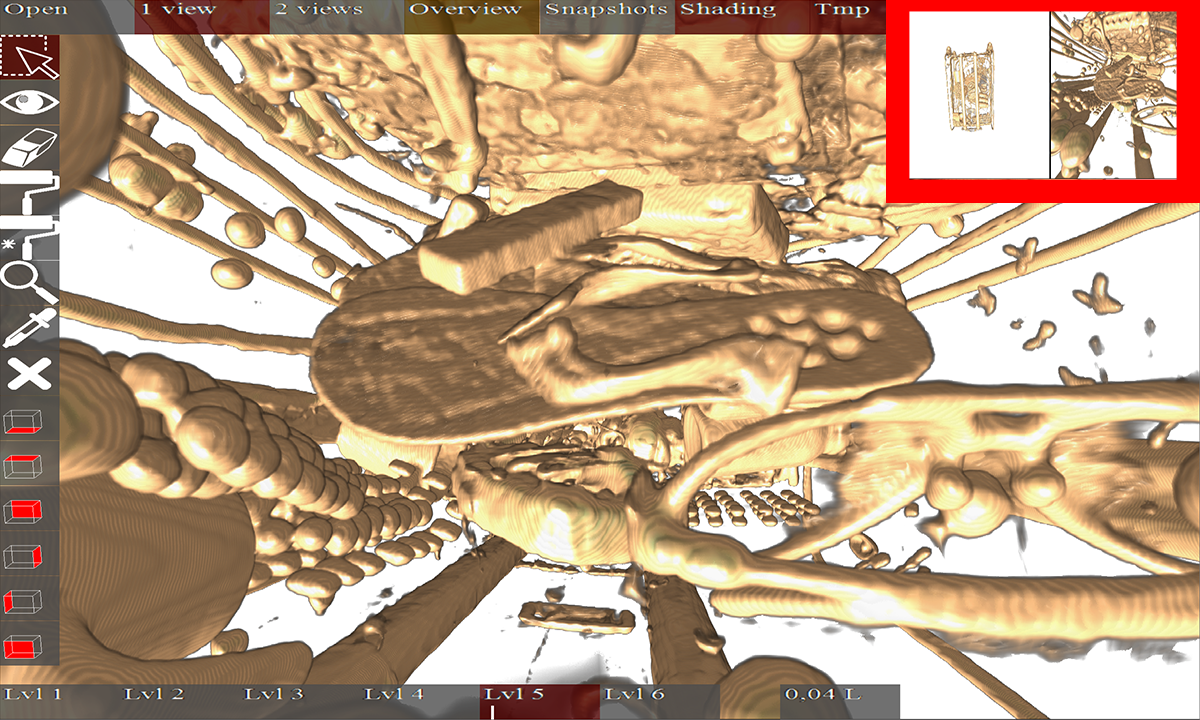
\includegraphics[width=9cm]{Figures/temporal.png}
	\caption{ The labelled snapshots taken by the user representing objects of interest}
	\label{f:temporal}
\end{figure}

\subsection{Possible Use Cases}

This section presents two scenarios that underline our system assets. The first scenario illustrates how users can explore a suspicious baggage and address occlusion to inspect items inside. The second scenario shows how to visualize the content of a closed metallic container. Currently, most airport don't use 3d systems, so we propose possible scenarios to highlight  how the usefulness of our interaction techniques.

\subsubsection{	Inspection of a suspicious baggage }
When a baggage arrives, the user sees it in its initial appearance which mainly shows the global structure . In order to better perceive its content, the user explores  the different transfer function presets. He or She clicks on the first level, then drags the cursors toward the others. This manipulation aims to reveal high density items hidden by those with low density 

(\autoref{f:scenario1_1}).
\begin{figure}
\centering
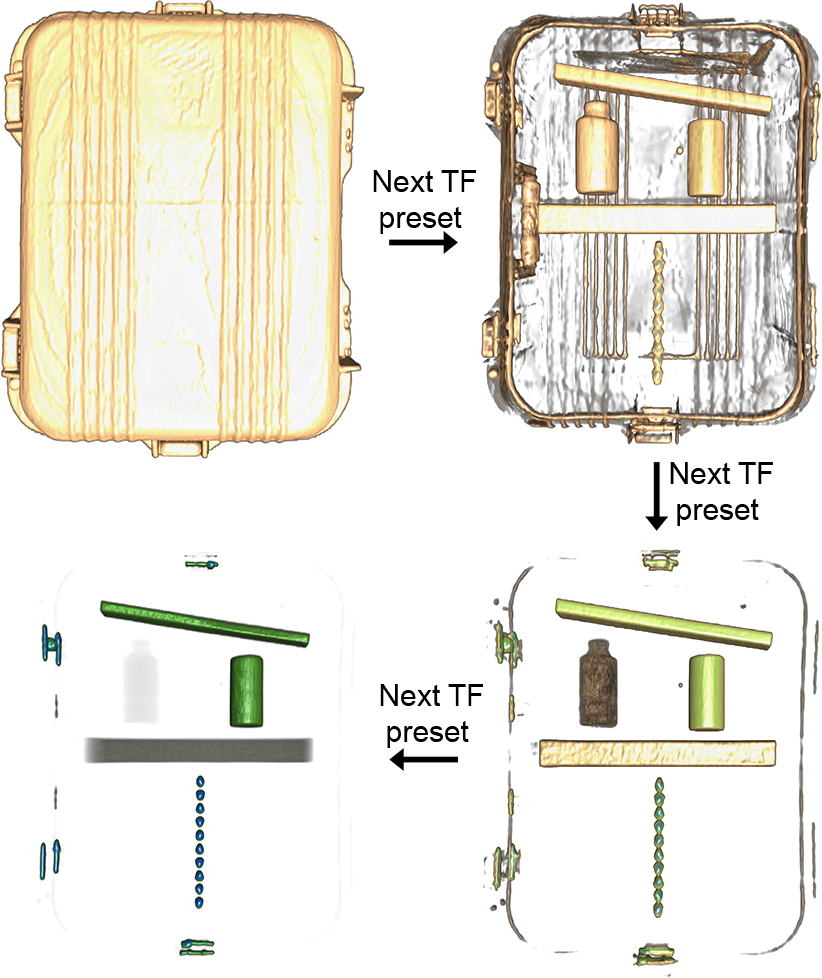
\includegraphics[width=9cm]{Figures/scenario1_1.png}
\caption{ The transfer function presets help the user perceive the different types of material inside the baggage }
\label{f:scenario1_1}
\end{figure}    
Once the user has a global understanding of the baggage, it seems to be a parcel bomb. So he or she decides to further inspect some specific areas. For instance, the user focuses an object which looks like an explosive material. To estimate the potential damages that could be caused by this potential threat, the security agent lock the camera on it. This object is now the main object of interest, and all  manipulations (e.g. translation, rotation) are now done around this object. This object of interest stays visible even if other items are in front of it (\autoref{f:menace}). 

\begin{figure}
\centering   
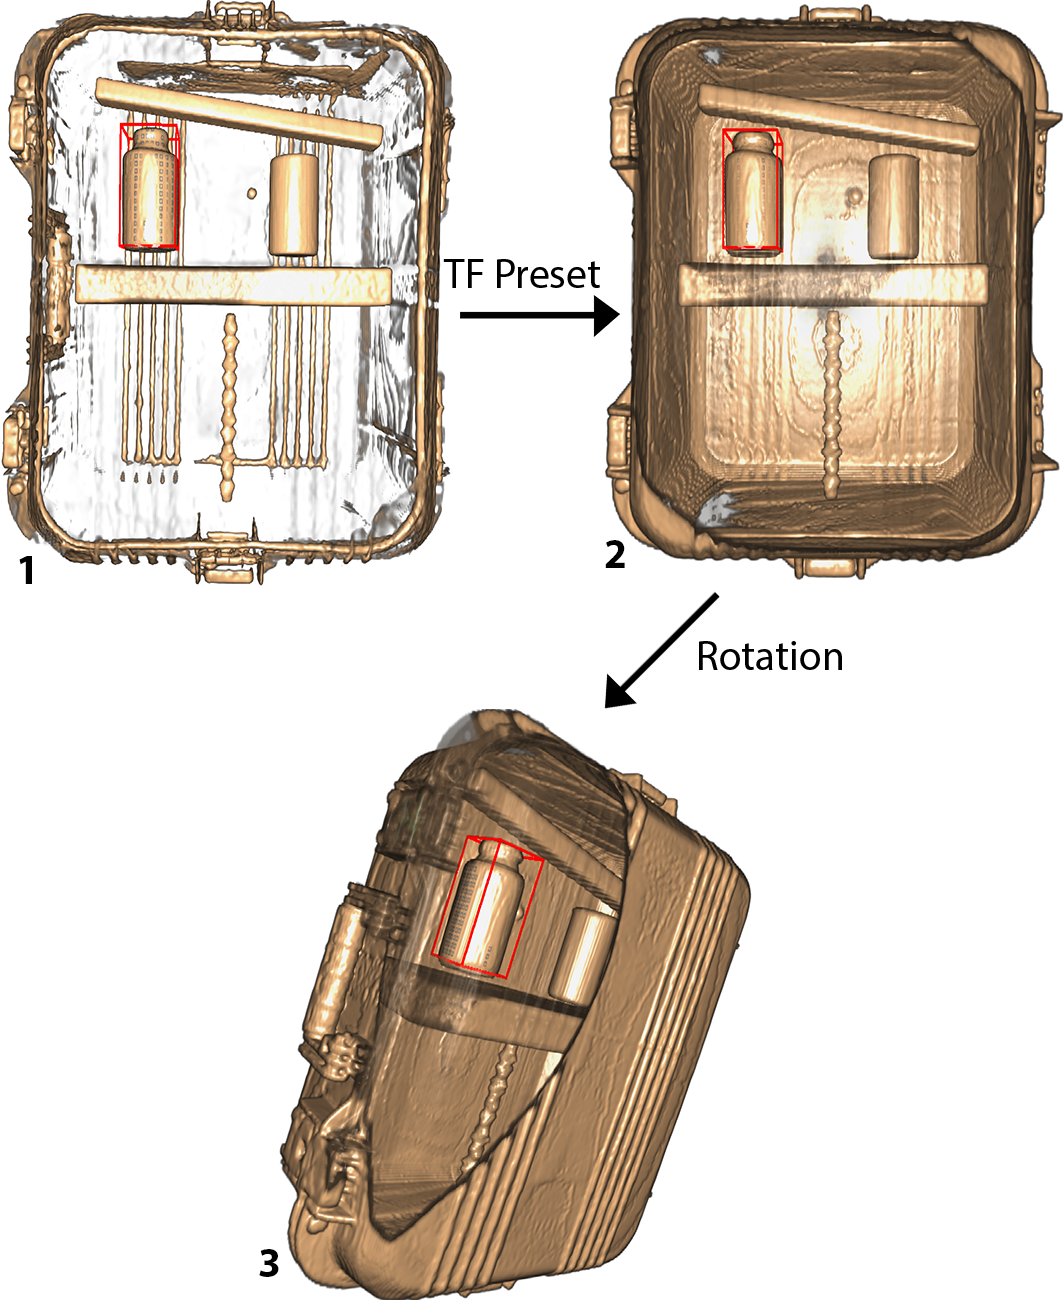
\includegraphics[width=9cm]{Figures/menace.png}
\caption[Inspection of an object from different perspectives.]{ Inspection of an object from different perspectives. 1- The user defines an object of interest for further inspection. This object is then inside a box with red borders. 2-  The user modifies the transfer function to see the target in another context. 3- The user rotates the baggage to look at the menace from a different perspective. It stays visible whatever the manipulation carried out.  }
\label{f:menace}
\end{figure} 


After the user finished this contextual inspection, he or she decides to inspect this object alone. To do so, the user selects it, and enables the second view. More information such as density and volume are displayed (\autoref{f:scenario1_3}).
\begin{figure}
\centering
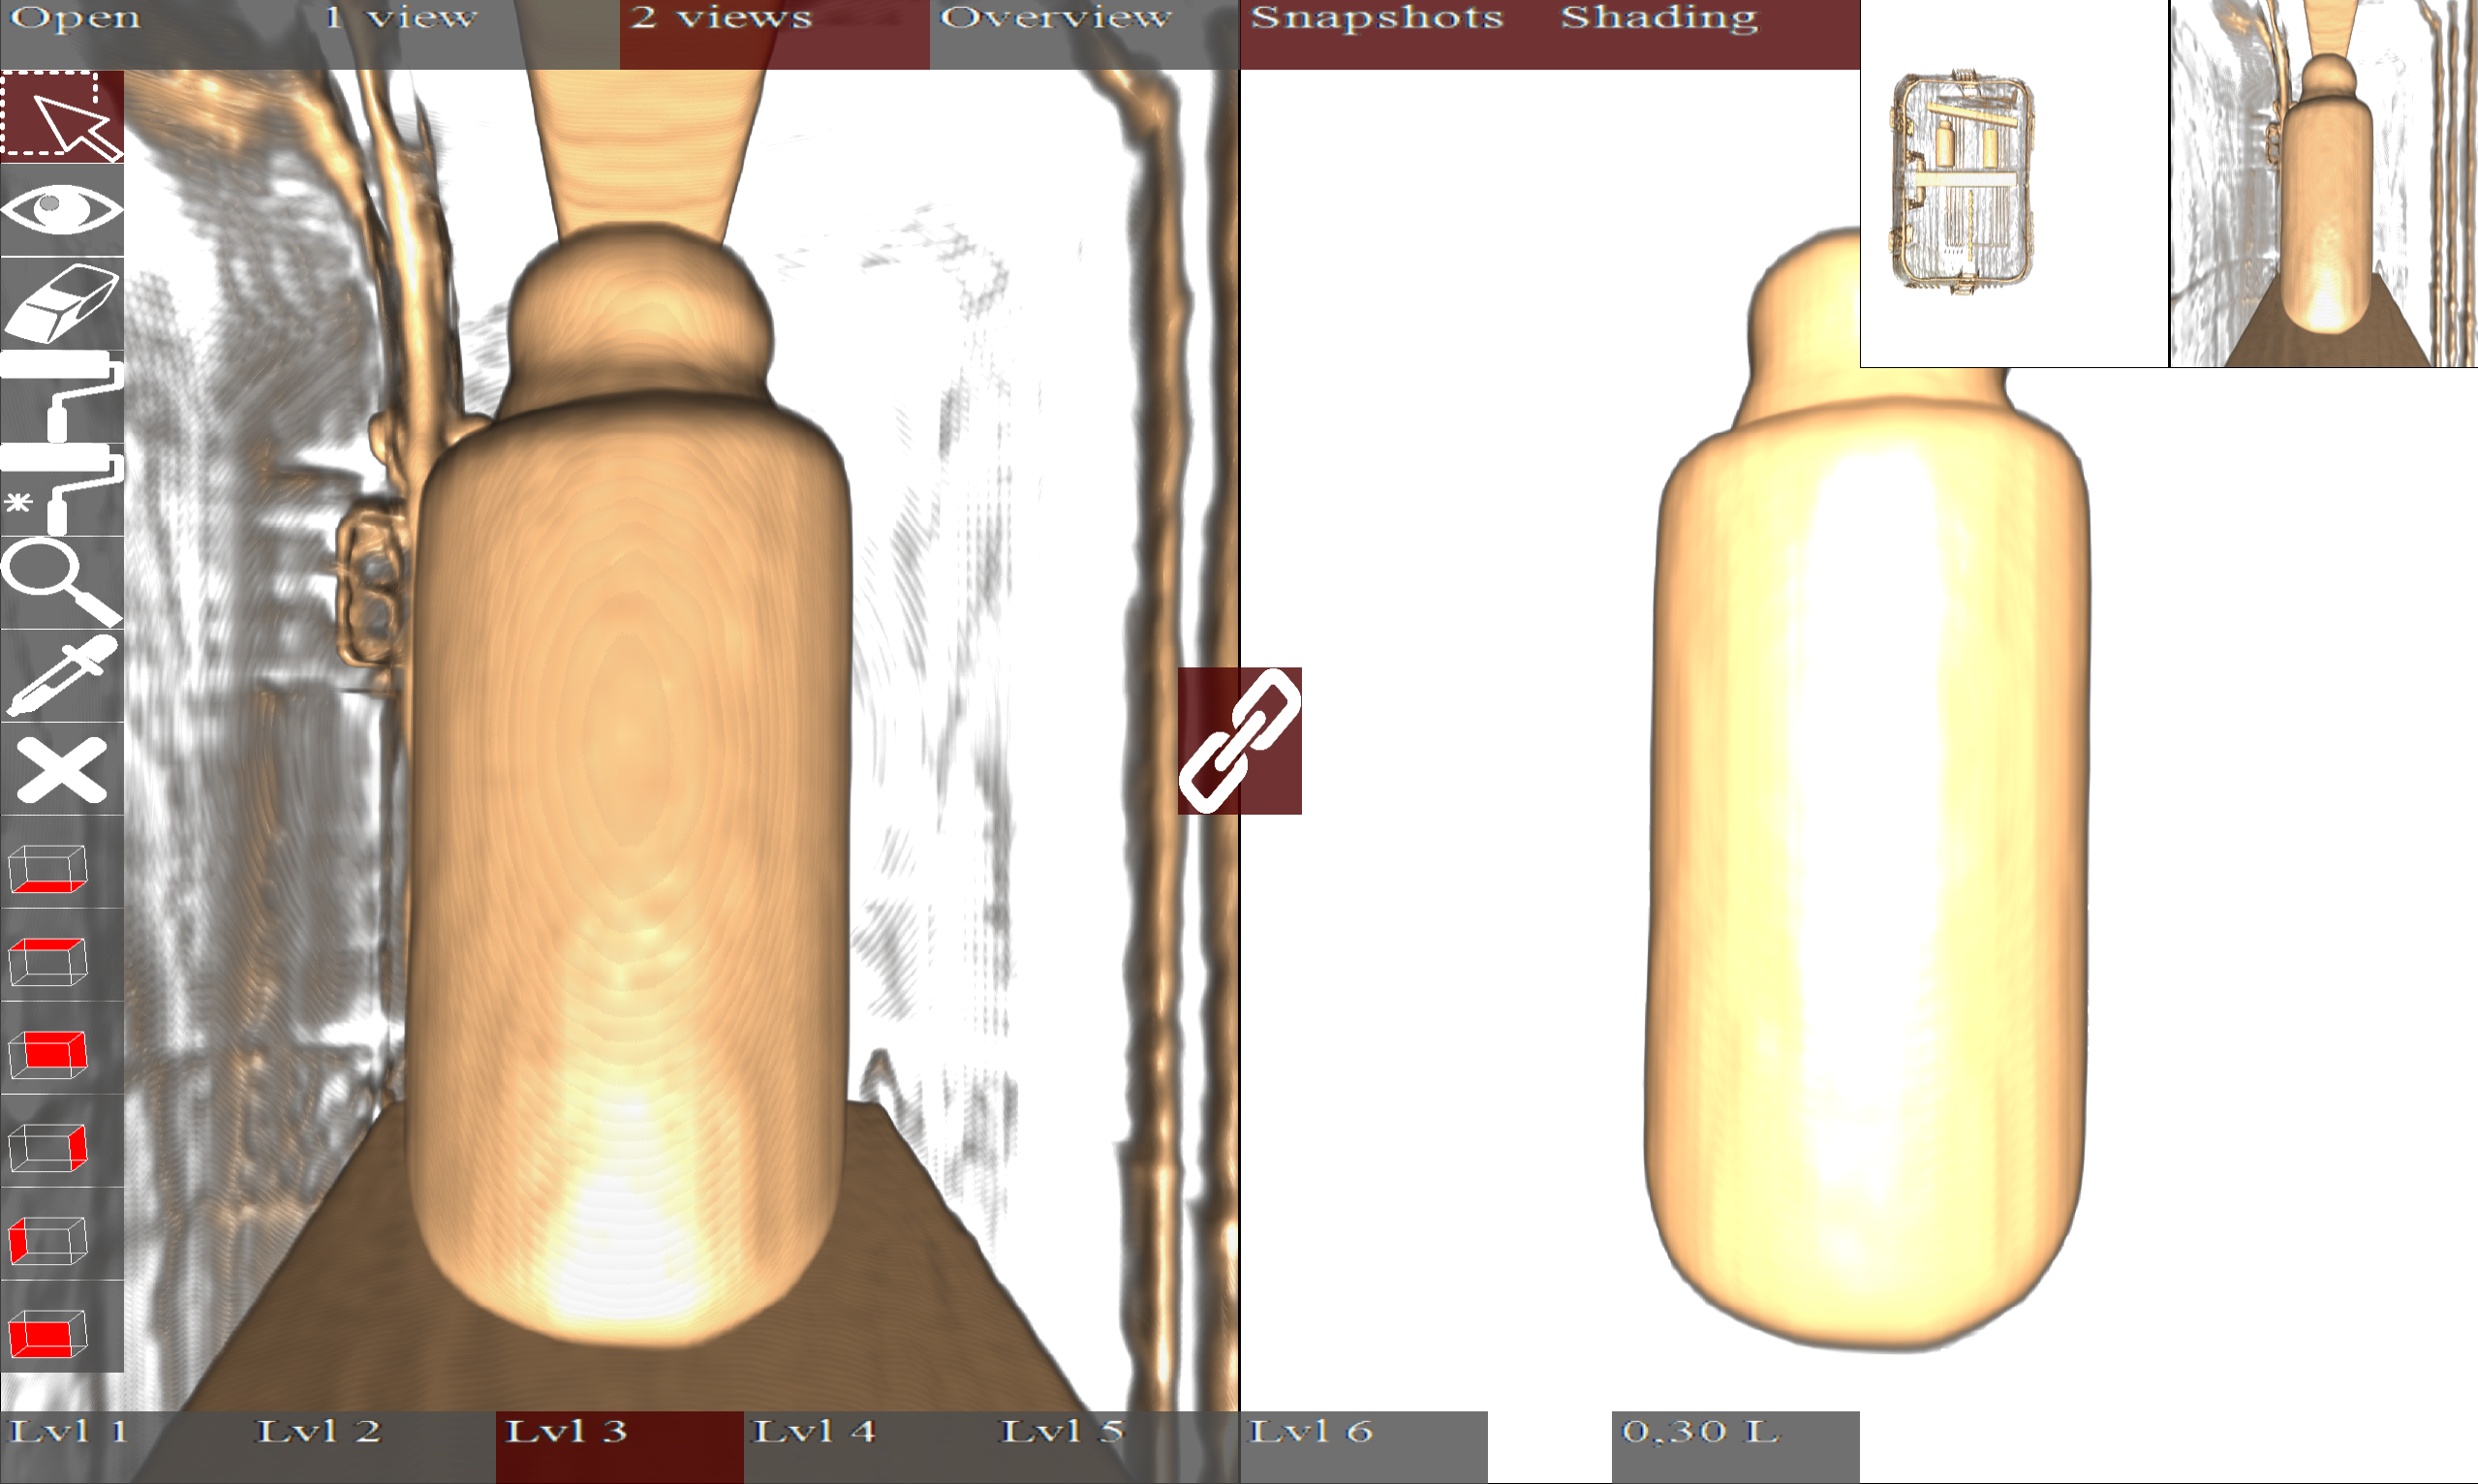
\includegraphics[width=7cm]{Figures/scenario1_3.PNG}
\caption{ A suspicious object is inspected apart of the rest of the baggage }
\label{f:scenario1_3}
\end{figure}

\subsubsection{Inspection of a big metallic object}

In this scenario, the user inspects a baggage featuring many visual artifacts which could be considered as noise (\autoref{f:scenario2_1b}). These spikes are created by the reflection of the x-rays on the heavy materials. Therefore, these visual artefacts are a hint indicating the presence of large metallic object. The user navigates through the different transfer function presets (\autoref{f:scenario2_2}) .
 
\begin{figure}
\centering
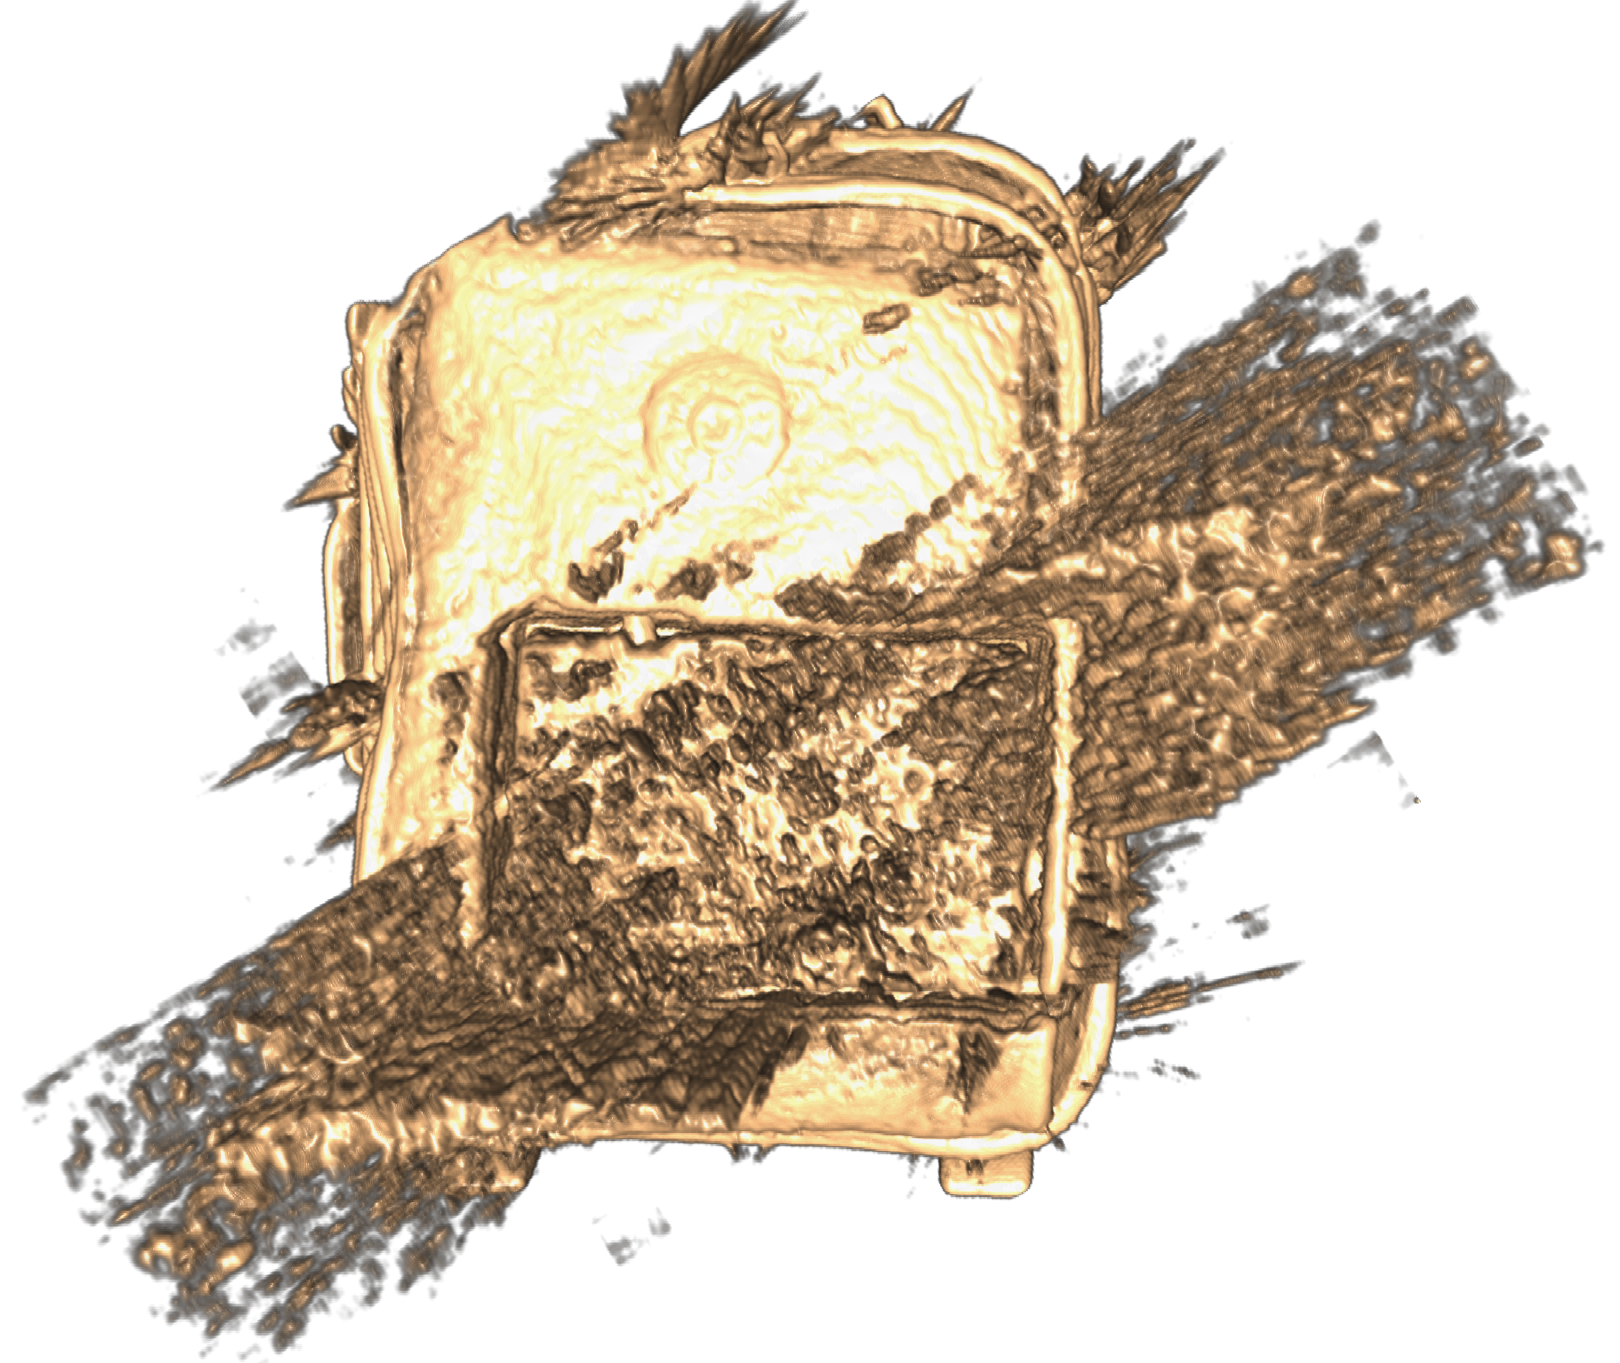
\includegraphics[width=9cm]{Figures/scenario2_1.PNG}
\caption{ Noise due to the presence of a big metallic object }
\label{f:scenario2_1b}
\end{figure}
After the selection of the adequate transfer function setting, he or she decides to farther inspect this metallic object. To do so, the user selects it with a double clicking on it. This object seems to be an engine.
\begin{figure}
\centering
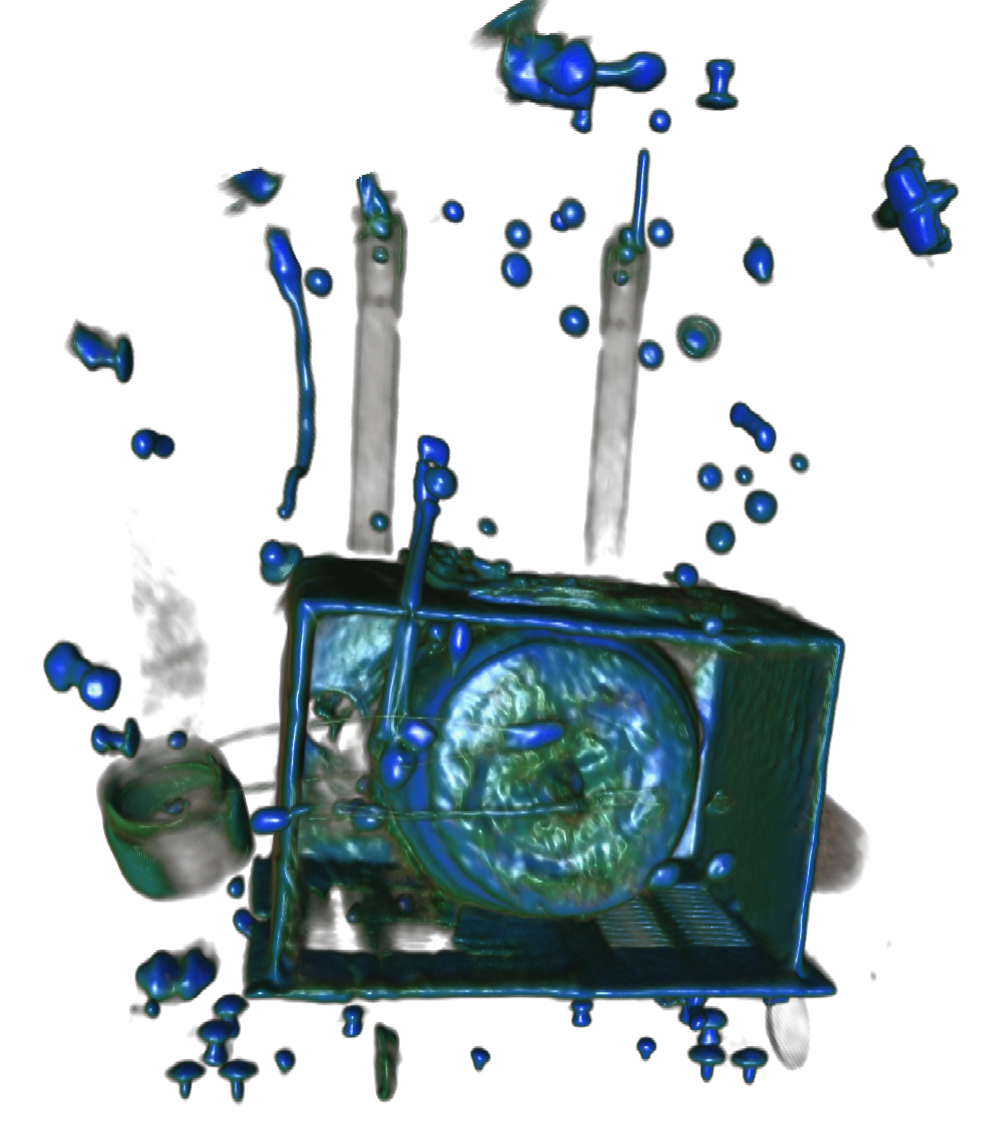
\includegraphics[width=9cm]{Figures/scenario2_2.PNG}
\caption{ The baggage actually contains  an engine }
\label{f:scenario2_2}
\end{figure}

In order to find out whether this engine is empty or not, the user decides to brush its half and to see its content. The user activates the brush tool, and while holding down the right button of the mouse, he or she brushes to remove the undesired section. After the brushing is carried out, the user modify the transfer function to show the lowest densities(\autoref{f:scenario2_1}).
\begin{figure}
\centering
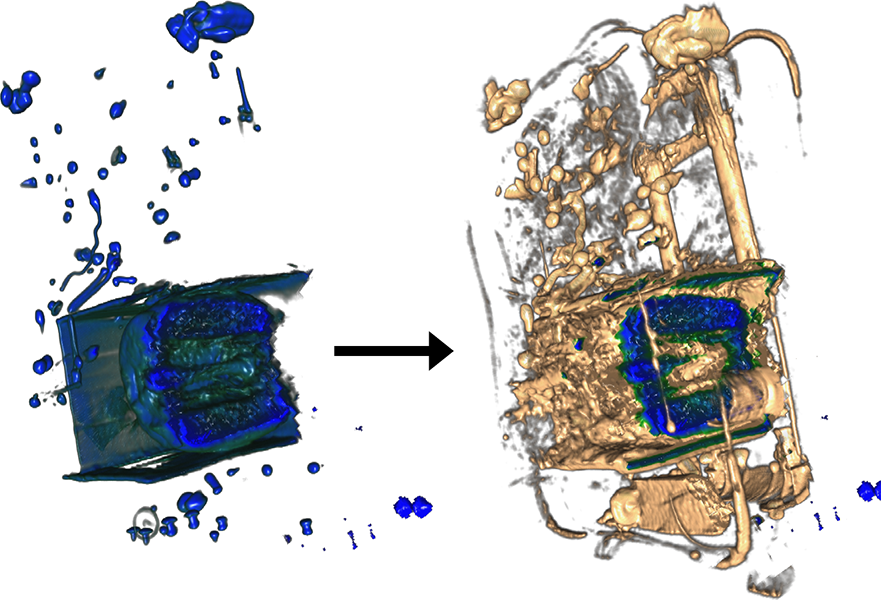
\includegraphics[width=\textwidth]{Figures/scenario2_3.png}
\caption{ the user reveals some low density materials inside the engine }
\label{f:scenario2_1}
\end{figure}


\subsection{Technical Constraints and Implementation}

Tomographs generate files which contain all the densities encountered by the x-rays through the baggage. These files usually contains around 30 million values. To load and to display such dataset in an interactive system, we used the parallel computation power of the graphic card. We used a program written in C\# combined with the CUDA parallel computing platform and a set of GPGPU techniques. To display the dataset, we used a standard ray casting algorithm. The contributions of you work rely on new interactions and their associated algorithms. This section will detail their implementations.

\subsubsection{Object selection}

Our software features interactive selection and voxel manipulation functionalities. To implement these interactions, we had to find a way to extract objects from the volume data. To do so, we explored many object detection algorithms such as contour trees by \cite{carr_computing_2000} and branch trees by \cite{pascucci_multi-resolution_2004} algorithms. But, according to the literature and our experience, these algorithms are computationally expensive and time-consuming especially during the preprocessing steps. In addition, this algorithm needs many settings and modifications to process the variety of available possible items which compose a baggage. For these reasons, we developed our own selection algorithm. It is based on a simple brute force multi-threads propagation algorithm. The first step consists in casting a single ray toward the volume data where the selection need to start.
Consider the typical DVR algorithm: Given a scalar volume $V \subset \mathbf{R}^3 \rightarrow \mathbf{R}$, each pixel $\mathbf{x} \in I$ in the DVR image $I \subset \mathbf{R}^2$ thereof corresponds to the compositing of sampled data along a ray that passes through $V$ and ends at $\mathbf{x}$. Such rays are defined by the eye position $\mathbf{e}$ and a ray direction unit vector
\begin{equation}
\mathbf{d} = \frac{ (\mathbf{x} - \mathbf{e}) }{ \| \mathbf{x} - \mathbf{e} \| }
\end{equation}
as the equation of a ray passing through a pixel is :
\begin{equation}
\mathbf{x}(t) =  \mathbf{e} + t\mathbf{d}
\end{equation}
where $x$ is the float-point location of the window corresponding to the pixel.
 We stop its progression as soon as it hits a visible voxel.



Second, we propagate the selection in every directions. For each encountered voxel, we check whether it is visible according to the current transfer function . If the voxel is visible we go on with the selection propagation. We spread within the baggage by launching many threads starting from the location where the first visible voxel has been hit. The number of thread depends on the number of logical processors inside the current hardware. Each thread checks whether its neighbors are visible, and keep spreading towards the visible voxels. This propagation algorithm stops whenever there are not any more visible voxels to spread into ( algorithm \autoref{alg:propagation}).

\begin{algorithm} \caption{Pseudo code for the selection propagation} 
\label{alg:propagation}
\begin{algorithmic}[1]
\Require $V$ the volume

\State Cast a ray toward the volume $V$  
\State  pt $\leftarrow$ intersection point between the ray and the volume \;
\State  finished $\leftarrow$ false \;
 \If{pt exists}
 	\State step $\leftarrow$ direction toward the volume \;
    \While{pt is inside the volume and $!$ finished }
  	\State color $\leftarrow$ the color at pt \;
  \If{color.alpha $>$ 0 }
	\State \emph{// spread into neighbors}
    
    \State v $\leftarrow$ current voxel \;
	\While{ v has neighbors }
    	\State color $\leftarrow$ voxel's color \;
        \State grad $\leftarrow$ voxel's gradient\;
    	 \If{color.alpha $>$ 0 and grad $<=$ threshold }
         \State 	v.selected $\leftarrow$ true \;
         \EndIf
        \State  v $\leftarrow$ next neighbor \;
    \EndWhile    

    \State finished $\leftarrow$ false;
    
  \EndIf
 \State  pt $\leftarrow$ pt + step \;
\EndWhile
 
\EndIf

\end{algorithmic}
\end{algorithm}




\subsubsection{Occlusion minimization}

Once the item of interest is selected, our system animates the visual configuration to display a new point of view of the selection which minimizes object occlusions. To do so, the system first computes the selection bounding box composed of six faces. Then, the system computes the six possible point of views. For each of them, the system counts the number of visible pixels which display the selected object. This is done thanks to the ray casting algorithm which propagates though the data cube and thus can test if the ray hits the selected items without any occlusion. Finally, the system defines the appropriate point of view as the bounding box face with the highest number of visible pixels of the selected item.
The system can then animate the volume visualization toward this new visual configuration and update the two temporal instances (before and after the pan, zoom and rotation modifications).

\subsubsection{Extended brushing technique}

The extended brushing techniques help the user explore the volume without modifying the transfer function. This interaction is also based on the ray casting algorithm. We only cast the rays located inside the radius of the brush in a parallel way.
When a ray hits a visible voxel whose density is within the brushing range, this voxel is then removed. If the voxel density is not in the brushing range, the ray casting algorithm stops.
The cancellation of the brushing is quite similar to the previous algorithm. The rays start from the back of the volume toward the front instead of front-to-back. The second difference consists in restoring the voxels whose density is inside the range.

\subsection{Discussion and conclusion}

Since we developed this system with four baggage security practitioners, we had the opportunity to validate the usefulness of each developed technique. Through an interactive process, the users gave their feedbacks all along the development process which helped to assess and to guide the proposed interaction techniques. Feedback was mainly positive and the user did not face any specific difficulty to use our system. Users mainly appreciated the simple interface with few widgets and the reduced set of interactions. Surprisingly, users were very interested to use the transfer function. The histogram and its transfer function were also appreciated even if the corresponding technique is not simple to understand. We suppose that our interface motivates users to learn more regarding the technique behind it. Users also mentioned the need to display the actual density (the numerical value) of selected object. They also ask many times if the displayed color corresponds to the one currently in use in operational settings. This confirms the fact that users are willing to keep some existing features and prefer to use a system they are already familiar with.
The users also appreciated our design requirements with smooth transitions and incremental investigations of baggage.
\par All of these observations and qualitative evaluations deserve to be validated through proper evaluations which are out of the scope of this user study paper.
Our system is fully functional and interactive enough to perform baggage explorations. Many improvements can still be done in order to improve its usages in terms of new interactions and exploration time reductions.
Technically speaking, the selection of the adequate point of view can be improved with more than 6 investigated faces. But in practice, this simple paradigm remains suitable. If the computed point of view is not fully satisfactory, one can manual rotate the baggage. Nevertheless, the developed algorithm will not necessary provide the best solution (the lowest occlusion) but a satisfactory one.
\par Our goal was to develop
innovative interactions to support baggage exploration but we did not really took into account the optimization of the exploration duration time. Manipulating the 3D volume may take time as well as our new interaction techniques. We think that these techniques have a great potential but they are suitable to explore in more details a suspicious baggage. Existing investigation techniques (with the 2D flattened image) are suitable to quickly and efficiently detect ''clean'' baggage. Then our tools can be a good solution to further investigate a potential threat with more available time.
\chapter{Interactive obstruction-free lensing for volumetric data visualization}
\label{lensing}

\section{Synthèse}

Le rendu direct de volume (DVR) est une technique de visualisation omniprésente pour afficher des champs scalaires 3D avec des applications en ingénierie, en sciences des matériaux et en imagerie médicale. Bien que largement adopté et capable de gérer des ensembles de données volumineux de manière interactive, le DVR souffre intrinsèquement du problème de l' \emph{occlusion}: les structures d’intérêt situées au fond du volume, appelées dans la suite \emph{cibles}, peuvent être difficiles à repérer et/ou explorer.


Pour y remédier, diverses techniques ont été conçues, notamment les fonctions de transfert, la segmentation, la sélection et le découpage. Cependant, toutes ces techniques ont des limites. Les mécanismes \emph{Globaux}, comme l'édition des fonctions de transfert, peuvent supprimer les objets gênants et les cibles s'ils ont des densités similaires. Dans certaines applications, des fonctions de transfert soigneusement conçues existent et doivent être utilisées sans modifications (significatives) pour faciliter la compréhension et la formation des utilisateurs \, \cite{4276082}. Les mécanismes \emph{Locaux} tels que la segmentation, la sélection ou le découpage sont plus efficaces pour manipuler les données confinées dans une région spatiale donnée. Cependant, beaucoup de ces mécanismes supposent que l'on peut facilement et précisément sélectionner des cibles pour les supprimer ou les conserver. Cela est difficile à faire lorsque \emph{par exemple} on n’a pas d’accès direct aux cibles, ou quand une interaction 3D importante est nécessaire pour sélectionner un ou des objets gênants.

Une autre façon de gérer l'occlusion consiste à utiliser des \emph{lentilles}. Ce sont des outils légers et flexibles qui permettent aux modifications locales et temporaires de révéler des cibles tout en conservant le contexte de visualisation global, \cite{595268, CGF:CGF12871, 6327262}. Cependant, la sélection efficace de la cible et la suppression de tous les objets gênants intermédiaires constituent toujours un défi. Plus précisément, la plupart des techniques de gestion d'occlusion existantes ne répondent pas simultanément à toutes les exigences suivantes: Créer rapidement une vue non obstruée de la cible (R1), permettre une exploration locale flexible de la zone cible (R2), conserver le contexte dans lequel la cible est visuellement comprise (R3), et gèrer les ensembles de données où la cible et les objets gênants ne peuvent pas être séparés par des manipulations de la fonction de transfert (R4).

\subsection{Contribution}
Nous proposons une nouvelle technique qui associe un rendu volumique de haute qualité à une lentille rapide, polyvalente et facile à utiliser pour prendre en charge l'exploration interactive des données sujettes à l'occlusion dans les volumes. Dans la classification des déformations de proposée par \cite{595268}, nous utilisons une distorsion radiale non linéaire à travers une lentille interactive pour supprimer les éléments occlusifs et conserver le contexte global tout en grossissant un élément partiellement occulté. En ce qui concerne les techniques de lentilles volumétriques, nous présentons notre contribution comme suit: Nous proposons une lentille de déformation interactive qui grossit et écarte les objets occlusifs situés devant un point focal désigné qui répond aux quatre exigences; la combinaison du changement interactif flexible et en temps réel du point focal, des rayons courbés personnalisés utilisés pour rendu volumique, la déformation de la lentille et de la fonction de transfert dans la zone cible, sans avoir à modifier le point de vue ou à manipuler des paramètres complexes dans plusieurs vues liées.

\subsection{Principe}

Considérons l’algorithme typique de DVR: Étant donné un volume scalaire $V \subset \mathbf{R}^3 \rightarrow \mathbf{R}$, chaque pixel $\mathbf{x} \in I$ dans l’image DVR $ I \subset \mathbf{R}^2$ correspond à la composition des données échantillonnées le long d'un rayon qui traverse $ V $ et se termine à $\mathbf {x}$. En DVR classique (\autoref{f:fisheyefr}-a), ces rayons sont définis par la position de l'oeil $ \mathbf{e}$ et un vecteur unitaire de direction du rayon
\begin{equation}
\mathbf{d} = \frac{(\mathbf{x} - \mathbf{e})}{\| \mathbf{x} - \mathbf{e} \|}
\end{equation}
. Considérons maintenant un point focal $\mathbf{f} \in I $ (le centre de la lentille) avec un rayon $ R> 0 $. Nous modifions tous les rayons traversant la lentille (focus/0 zone $D = \{\mathbf{x} \in I | \| \mathbf{x} - \mathbf{f} \| \leq R\}$ pour enlever l'occlusion, magnifier et accentuer un objet cible. Notre comportement de rayon est divisé en trois étapes: (1) Fournir une vue claire de la cible en se en rapprochant et en poussant les objets gênants de côté. (2) Définir large un champ de vue (fisheye) pour mieux voir la cible. (3) Modifier les paramètres de la lentille, de l'éclairage et de l'opacité de la TF en temps réel pour mieux explorer la cible.

\begin{figure}
\centering

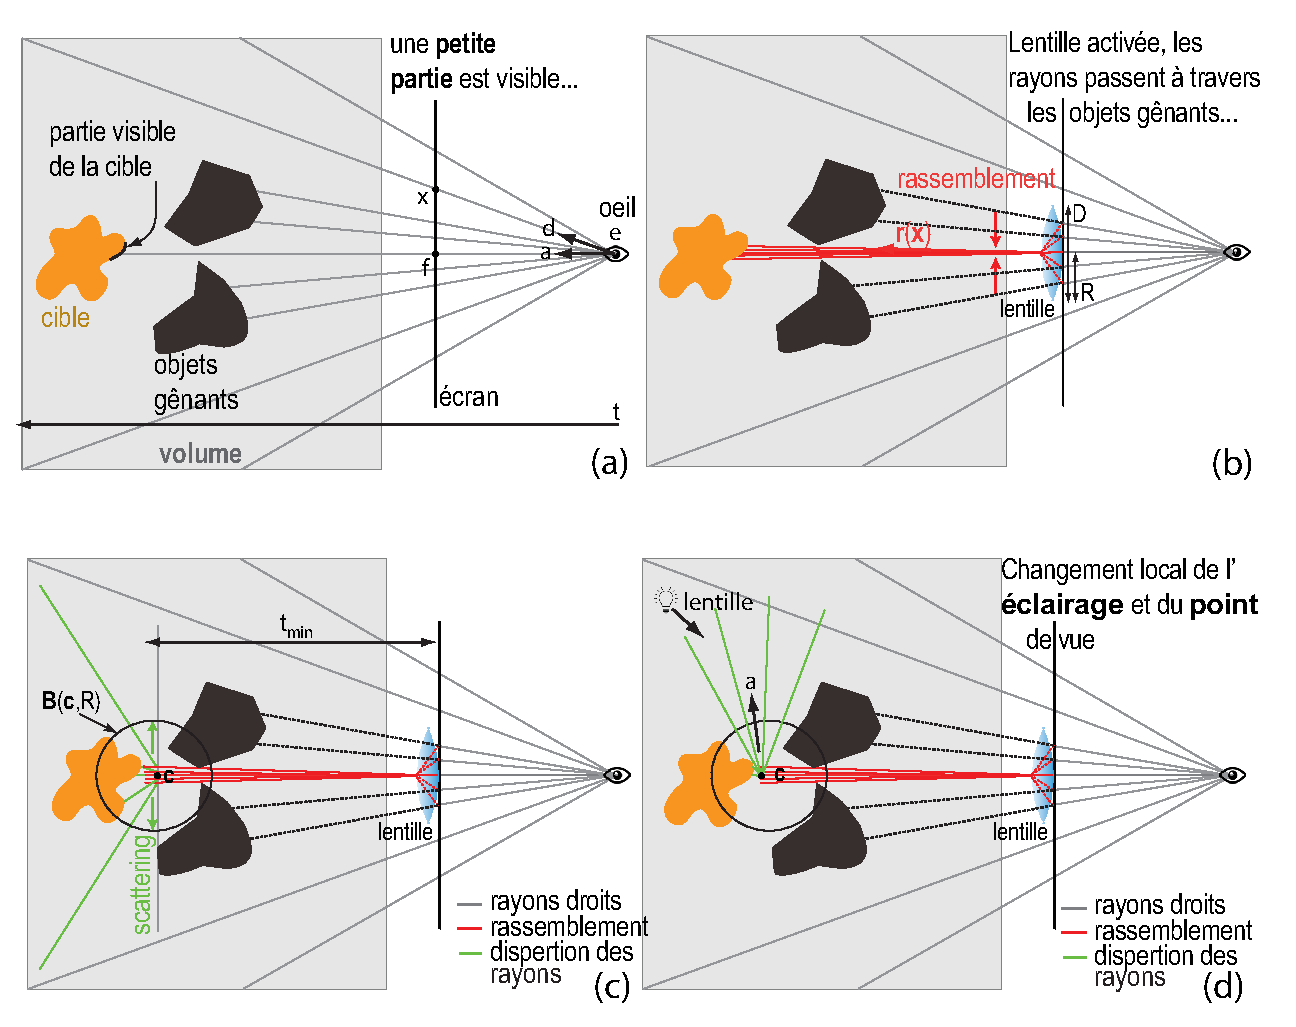
\includegraphics [width=\textwidth]{images/principlefr.eps}

\caption[Fonctionnement de la lentille sans occlusion]{Fonctionnement de la lentille sans occlusion. Une cible est (principalement) cachée par des objets gênants devant elle. (a) Le DVR classique affiche une petite partie de la cible. (b) Notre lentille recueille des rayons pour éviter les objets gênants. Une fois près de la cible, les rayons suivent à nouveau leurs trajectoires initiales. Cependant, seule une petite partie de la cible est visible. (c) Les rayons se dispersent et  rendent toute la cible visible. Enfin, nous ajustons les directions de visualisation et d'éclairage locales $\mathbf{a}$, $\mathbf{l}^{lens}$.}
\label{f:fisheyefr}

\end{figure}



\subsubsection{Créer une vue dégagée}

Le scénario que nous traitons est le suivant: Avec un volume $ V $, les utilisateurs en produisent un DVR, en utilisant tous les TF appropriés et les autres paramètres applicables. Lors de l'exploration de $V$ à partir de divers points de vue, (au moins) un point de vue $ (\mathbf{e}, \mathbf{d}) $ est trouvé, d'où une structure intrigante est \emph{partiellement} visible dans $ I $. Nous appelons cette structure \emph{cible}. Les utilisateurs veulent ensuite démêler rapidement et facilement la cible. Pour cela, nous procédons comme suit: Nous commençons par \emph{rassembler} tous les rayons traversant les pixels de la lentille (zone d'intérêt $ D $) pour suivre le vecteur de l'axe de la lentille.

\begin{equation}
 \mathbf{a} = \frac{(\mathbf{f} - \mathbf{e})}{\| \mathbf{f} - \mathbf{e} \| }
 \end{equation}
 . Comme expliqué ci-dessus, à l'emplacement $ \mathbf{f} $ du centre de la lentille, nous voyons une cible intéressante partiellement cachée. Par conséquent, par définition, les rayons recueillis passent \emph{à travers} des objets gênants pour atteindre cette cible, sinon nous ne la verrions pas. Nous contrôlons le rassemblement en définissant la direction des rayons passant par $ \mathbf{x} \in D $ à
%
\begin{equation}
\mathbf{r}(\mathbf{x}) = (1- \alpha) \mathbf{a} + \alpha \mathbf{d},
\label{eqn:collecte}
\end{equation}
%
avec $ \alpha \in [0,1] $. Lorsque $\alpha = 0 $ (valeur par défaut), tous les rayons suivent l'axe de la lentille $ \mathbf{a} $ et peuvent donc mieux traverser les obstacles. Lorsque $ \alpha = 1 $, les rayons suivent une trajectoire droite. Changer $ \alpha $ avec la molette de la souris navigue en douceur entre l'effet de l'objectif, \emph{i.e.} ouvrir un "trou" dans le volume pour voir la cible et le DVR classique.

\subsubsection{Définir un large champ de vision}
Une fois que les rayons passent des obstacles (\autoref{sec: réunion}), nous voulons les \emph{les disperser} afin de mieux échantillonner la cible. Considérez que cette cible est à une certaine profondeur $ t_{target}> 0 $ dans $ V $. Après que les rayons aient passé les objets gênants, mais avant qu'ils n'atteignent la cible, \emph{ie}, passez au-delà d'une distance $ t_{min} <t_ {cible} $ à $ V $, nous les dévions au mieux échantillonnez la cible. Pour cela, nous définissons la position paramétrique d’un point de rayon sur
%
\begin{equation}
\mathbf{p}(\mathbf{x}, t) = \mathbf{r}(\mathbf{x})t + \beta (\mathbf{x} - \mathbf{f}) (t-t_{min})
\label{eqn:diffusionfr}
\end{equation}
%
pour tout pixel $ \mathbf{x} \in D $ et tout $ t \geq t_{min} $. Ici, $ \beta \geq 0 $, ajusté via la molette de la souris tout en appuyant sur la touche Shift (\autoref{f:fisheyefr}-c), contrôle la diffusion des rayons: les petites valeurs agrandissent une petite zone de volume proche du rayon $\mathbf{r}(\mathbf{x}) $; des valeurs plus importantes échantillonnent davantage le volume derrière la lentille. Intuitivement, c'est comme si nous avions déplacé une loupe à une profondeur $ t_{min} $ dans $ V $. En résumé, après que l'utilisateur ait trouvé une cible intéressante mais partiellement fermée à l'aide du \emph{standard} DVR, notre lentille serre les rayons pour passer entre les objets gênants et les projette ensuite pour explorer la cible.

\subsubsection{Exploration interactive de la cible}
\begin{figure}
\centering

\includegraphics [width=\textwidth]{images/params.eps}

\caption[Modification des paramètres d'éclairage dans la lentille.]{Modification des paramètres d'éclairage dans la lentille. (a) Coefficient spéculaire globlal constant. (b) Coefficient spéculaire élevé dans la lentille et faible en dehors. (c-f) La modification du vecteur lumière à l'intérieur de la lentille  produit l'effet d'une lampe de poche tournant autour de la cible.  Les icônes de la balle illustrent la direction du vecteur de lumière locale.}
\label{f:paramsfr}

\end{figure}


Pour réaliser une exploration plus efficace, nous pouvons modifier de manière interactive plusieurs paramètres du DVR et de la lentille, comme suit.


\par \textbf{Rayon de la lentille:} Le rayon $ R $, indiquant la taille du "trou" à ouvrir dans le volume pour voir la cible, est défini via la molette de la souris. Les paramètres $ \alpha $ et $ \beta $ (affectant respectivement la collecte et la diffusion des rayons) sont définis par la molette de la souris et les touches de modification. La valeur $ t_{min} $ (profondeur à partir de laquelle la diffusion commence) est définie à l'aide des touches fléchées.

\par \textbf{Axe de l'objectif:} Les utilisateurs peuvent faire pivoter l'axe de la lentille $ \mathbf{a} $ en utilisant un trackball virtuel activé par le bouton droit de la souris. Changer $ \mathbf{a} $ échantillonne effectivement la cible à partir de nombreux points de vue, permettant à l'utilisateur de regarder autour d'elle pour voir les parties non visibles du point de vue actuel, mais \emph{sans changer} le point de vue. Ceci est une valeur ajoutée élevée, puisque le changement de point de vue peut nous amener à une vue où la cible est totalement invisible, nous ne savons donc pas exactement où activer la lentille. 

\par \textbf{Lighting:} Nous modifions les paramètres d'éclairage volumétrique de Phong pour mieux explorer la cible, comme suit. Soit
\begin{equation}
\mathbf{c} = \mathbf{e} + t_{min} \mathbf{a}
\end{equation}
 un point en profondeur $t_{min} $ le long de l'axe de lentille, et soit $ B(\mathbf{c}, R) $ une sphère de rayon $ R $ autour de ce point (\autoref{f:fisheyefr}-b ). Nous appelons les voxels dans cette sphère dans le 'focus', et tous les autres voxels dans $ V $ sont "flous". Soit $ \phi $ le coefficient du terme spéculaire, défini sur une valeur élevée (par défaut: un).
Premièrement, pour tous les voxels $ \mathbf{x} \in B (\mathbf{c}, R) $, nous utilisons un coefficient spéculaire
\begin{equation}
\phi(\mathbf{x}) = \phi (1-d)
\end{equation}
, où
\begin{equation}
 d = \frac{\| \mathbf{x} - \mathbf{c} \|}{R}
\end{equation}.
Pour tous les voxels en dehors de $ B (\mathbf {c}, R) $, nous utilisons $ \phi (\mathbf{x}) = 0 $. Par conséquent, les voxels proches du point focal $ \mathbf{c} $ apparaissent hautement spéculaires; plus loin de $ \mathbf{c} $, les voxels deviennent moins spéculaires et les voxels flous sont purement diffus. Deuxièmement, nous permettons à l'utilisateur de faire pivoter localement le vecteur de lumière en utilisant le même mécanisme de boule de commande que pour la rotation de l'axe de la lentille. Soit $ \mathbf{l}^{lens} $ ce vecteur, et soit $ \mathbf{l}^{global} $ le vecteur de lumière global utilisé par le DVR standard. Pour tous les voxels en question, nous utilisons un vecteur lumière
\begin{equation}
\mathbf{l}(\mathbf{x}) = (1 - d) \mathbf{l}^{lentille} + d \mathbf{l}^{global}
\end{equation}.
 
  Lorsque l'utilisateur effectue une rotation de $\mathbf{l}^{lens} $, la direction de la lumière changera visiblement au milieu de l'objectif, restera constante en dehors de celui-ci et se modifiera progressivement.


Les deux mécanismes ci-dessus combinés produisent l'effet d'une lampe de poche en mouvement tournant autour d'une cible brillante incorporée dans une scène diffuse constamment éclairée. \autoref{f:paramsfr} montre ces mécanismes pour un ensemble de données de scanner thoracique contenant une tumeur profondément enfouie. Nous voyons comment le fait de tourner la lumière met en évidence des détails à petite échelle sur la surface cible (tumeur) sans changer le point de vue ou la position de la lentille. De plus, la forte spécularité de la lentille attire l’attention de l’utilisateur sur cette zone; L'éclairage diffus à l'extérieur de l'objectif met moins l'accent sur la zone contextuelle.

\par \textbf{Opacité:} Nous modifions l'opacité de la fonction de transfert selon une idée similaire à celle utilisée pour l'éclairage. Soit $ TF_{o}^{global}: \mathbf{R} \rightarrow [0,1] $ la fonction d'opacité choisie par l'utilisateur et utilisée globalement pour le volume. Soit $ \gamma $  une impulsion gaussienne de la hauteur de l'unité centrée à la valeur de densité moyenne $ \bar{\rho} $ à $ B(\mathbf{c}, R) $ et avec un écart type $ \sigma $. Nous estimons $ \bar{\rho} $ et $ \sigma $ en considérant la densité $ \rho $ à 150 points échantillonnés aléatoirement dans $ B(\mathbf{c}, R) $. Des valeurs plus élevées pour le nombre d'échantillons donnent des résultats visuellement très similaires pour nos volumes testés pouvant atteindre 500$^3$ voxels, tout en nécessitant (légèrement) plus de coûts de calcul. Ensuite, pour les voxels dans $ B(\mathbf{c}, R) $, nous utilisons une fonction de transfert d'opacité efficace
\begin{equation}
TF_o = TF_{o}^{global} + (1-d) \gamma
\end{equation}.
 Pour les voxels en dehors de $ B $, nous utilisons $ TF_{o}^{global} $ (DVR standard).
Ceci est utile lorsque l'utilisateur définit $ TF_{o}^{global} $ pour rendre la plupart des voxels hors de la lentille relativement transparents. Dans ce cas, $ TF_o $ rendra les voxels opaques dans $ B $, permettant ainsi de mieux voir les structures en focus. \autoref{f:paramsfr} a été généré de cette façon.

\subsubsection{Transitions fluides}

Si nous plions des rayons traversant les pixels de la lentille $ D $ (\autoref{eqn:collecte} et \autoref{eqn:diffusionfr}) et des rayons commençant à des pixels de $ I \setminus D $ comme des droites, des discontinuités apparaissent au bordures d'objectif. Nous résolvons ceci comme suit. Soit $ \mathbf{p}(\mathbf{x}, t) $ les voxels le long d'un rayon de lentille commençant au pixel de l'écran $ \mathbf{x} $, calculé par \autoref{eqn:diffusionfr}. Soit $ \mathbf{p}^{line}(\mathbf{x}, t) $ les voxels le long d'un rayon linéaire commençant à $ \mathbf{x} $, \emph{ie}, calculé en utilisant $ \alpha = 1 $ et $ \beta = 0 $ dans \autoref{eqn:collecte} et \autoref{eqn:diffusionfr} respectivement. Pour chaque valeur $ t $ le long de chaque rayon, on calcule le rayon interpolé
\begin{equation}
\bar{\mathbf{p}}(\mathbf{x}, t) = (1-f(d)) \mathbf{p}(\mathbf{x}, t) + f(d) \mathbf{p}^{ligne}(\mathbf{x}, t)
\end{equation},
 où $ d $ est la distance de $ \mathbf{x} $ à l'axe de la lentille (normalisée à l'unité en la divisant par $ R $) et $ f: [0,1] \rightarrow [0,1] $ est une fonction d'interpolation. Ensuite, nous utilisons les rayons $ \bar{\mathbf{p}}(\mathbf{x}, t) $ pour calculer le DVR par composition standard. De cette façon, les rayons varient efficacement de leurs versions modifiées (près de l'axe de l'objectif) aux lignes droites (à l'extérieur de l'objectif). Le réglage de $ f(d) = d^2 $ maintient les transitions d'interpolation proches de la bordure de la lentille, de sorte que la majeure partie de la lentille soit dédiée à l'affichage de l'effet fish-eye souhaité.

Séparément, nous utilisons une animation de slow-in/slow-out \, \cite{Dragicevic:2011:TDA:1978942.1979233} pour introduire l'effet de la lentille. En activant la lentille, on fait varier les valeurs par défaut de $ \alpha $ et $ \beta $ ($ \alpha = 1 $, $ \beta = 0 $, \emph{c'est-à-dire}, DVR classique en ligne droite) à leur utilisateur réel. Définir des valeurs, calculer le rendu du volume à la volée et afficher les images résultantes. L'effet ressemble progressivement à l'ouverture d'un trou dans le volume. L'augmentation de la vitesse au début de l'animation permet de voir rapidement ce qui est révélé dans la lentille; la vitesse décroissante à la fin aide à voir où les objets gênants repoussés vont réellement. Cela donne également une certaine sémantique aux formes en mouvement, permettant d'interpréter le mouvement comme un grossissement d'une cible, et de garder le focus sur les entités visuelles pendant cette transition. Lors de la désactivation de la lentille, nous lisons l'animation dans le sens opposé, ce qui suggère de fermer le trou ouvert dans le volume.


Nous avons évaluer notre lentille avec des utilisateurs sur un scénario d'inspection de baggages. Selon les sujets, notre outil peut leur fournir une meilleure perception des articles à l’intérieur du bagage par rapport aux appareils à rayons X classiques à un seul point de vue qu’ils utilisent couramment. Cependant, notre outil ne doit pas être utilisé pour l'inspection typique des bagages à main, dont le temps d'inspection autorisé est très faible (15 à 20 secondes). Notre outil est beaucoup plus intéressant pour inspecter les bagages enregistrés, où les fenêtres d’inspection vont jusqu’à 3 minutes. La valeur ajoutée perçue pour ce cas d'utilisation est également plus élevée: l'ouverture des bagages enregistrés pour une inspection manuelle est beaucoup plus compliquée et longue que pour les bagages de cabine. De plus, le seul système d’inspection des bagages enregistrés que les sujets connaissaient est un scanner qui vise à \emph{détecter} automatiquement les menaces via des images radiographiques; ce système souffre de faux positifs, de sorte qu'un outil d'examen manuel comme le nôtre pourrait rapidement éliminer ces faux positifs, et donc les délais d'ouverture des bagages enregistrés. Enfin, plusieurs sujets ont suggéré qu’ajouter une fonction pour afficher une vue de coupe 2D classique (activée par une pression sur une touche et alignée avec le point focal) serait utile car cela donnerait des détails supplémentaires.



\NewPage






Occlusion is an issue in volumetric visualization as it prevents direct visualization of the region of interest. While many techniques such as transfer functions, volume segmentation or view distortion have been developed to address this, there is still room for improvement to better support the understanding of objects' vicinity. However, most existing Focus+Context fail to solve partial occlusion in datasets where the target and the occluder are very similar density-wise. For these reasons, we investigate a new technique which maintains the general structure of the investigated volumetric dataset while addressing occlusion issues. With our technique, the user interactively defines an area of interest where an occluded region or object is partially visible. Then our lens starts pushing at its border occluding objects, thus revealing hidden volumetric data. Next, the lens is modified with an extended field of view (fish-eye deformation) to better see the vicinity of the selected region. Finally, the user can freely explore the surroundings of the area under investigation within the lens. To provide real-time exploration, we implemented our lens using a GPU accelerated ray-casting framework
to handle ray deformations, local lighting, and local viewpoint manipulation. We illustrate our technique with five application scenarios in baggage inspection, 3D fluid flow visualization, chest radiology, air traffic planning, and DTI fiber exploration.

\section{Introduction}
Direct volume rendering (DVR) is a pervasive visualization technique for displaying 3D scalar fields with applications in engineering, material sciences, and medical imaging sciences. However widely adopted, and able to handle large datasets at interactive rates, DVR inherently suffers from the problem of \emph{occlusion}: Structures of interest located deep in the volume, called next \emph{targets}, can be hard to spot and/or explore.

To aid with this, various techniques have been designed including transfer functions, segmentation, selection, and clipping. Yet, all such techniques have limitations.  \emph{Global} mechanisms, like transfer function editing, can remove both occluders and targets if these have similar densities. In certain applications, carefully designed transfer functions exist and should be used without (significant) modifications to facilitate understanding and user training\,\cite{4276082}. \emph{Local} mechanisms like segmentation, selection, or clipping are more effective in manipulating data confined to a given spatial region. Yet, many such mechanisms assume that one can easily and accurately select targets to remove them (occluders) or keep them (occluded). This is hard to do when \emph{e.g.} one does not have direct access to the targets, or when significant 3D interaction is required to select occluder(s).

A different way to handle occlusion is to use \emph{lenses}. These are flexible lightweight tools which enable local and temporary modifications of the DVR to reveal targets while keeping the global visualization context, \cite{595268,CGF:CGF12871,6327262}. However, efficiently selecting the target and  removing all in-between occluders is still challenging. More specifically, most existing occlusion management techniques do not simultaneously meet all following requirements: Rapidly create an unobstructed view of the target (R1), allow a flexible local exploration of the target zone (R2), keep the context in which the target is visually embedded (R3), and handle datasets where the target and occluders cannot 
be separated by transfer function manipulations (R4).

In this chapter, we increase the flexibility of lenses for DVR exploration to jointly cover all above requirements. We propose a focus-and-context (F+C) lens that combines a distortion technique, which pushes aside the occluding objects, with a fish-eye field of view, to provide a better perspective on targets. We specifically target the use-case of \emph{partially occluded} objects, where the user has a glimpse of an interesting structure, buried deep in the data, but only slightly visible from a given viewpoint and transfer-function setting. We allow the user to ''open up'' the volume without changing these settings, and reveal the target, by simple point, click, and scroll operations. Next, we provide several F+C modifications of the lighting parameters, transfer function, and geometry in the focus area to better understand the target. Our technique, implemented using a CUDA-based approach, can be easily incorporated in any generic DVR system.

The chapter is structured as follows. \autoref{sec:requirements} presents again the four requirements for occlusion management in DVR visualization. \autoref{sec:principle} introduces the principle of our lens. \autoref{sec:implem} introduces implementation details.\autoref{sec:scenarios} presents five application scenarios for our lens in baggage inspection, 3D fluid flow visualization, chest radiology, air traffic planning, and DTI fiber exploration. \autoref{sec:discussion} discusses our proposal. Finally, Section~\autoref{sec:conclusions} concludes the chapter.

\section{Requirements}
\label{sec:requirements}

To start with, let us recall requirements R1$,\ldots,$R4.
\begin{itemize}
\item{\textbf{R1:}} The technique should rapidly create an unobstructed view of the target, \emph{i.e.}, such a view should be created at interactive frame rates (10 fps or more) with no special pre-processing of the input volume (\emph{e.g.}, segmentation), and with minimal user input (\emph{e.g.}, using simple mouse and/or keyboard-modifier events). All above are needed to ensure that one can freely \emph{explore} the volume by activating the lens anywhere with minimal effort and seeing its effect in real-time.

\item{\textbf{R2:}} Allowing a flexible exploration of the target zone means that one can manipulate the zone in the lens in various ways to see how the target is actually embedded in its surrounding context.

\item{\textbf{R3:}} Keeping the context means that the visualization around the lens does not change significantly from what would be shown there if the lens were not activated. This is needed to maintain the user's mental map before \emph{vs} after activating the lens.

\item{\textbf{R4:}} The lens should enable the exploration of datasets where targets cannot be easily separated (isolated) from their surrounding context simply by manipulating parameters of the transfer functions (TF). One such issue is when targets and surrounding zones have similar densities; in this case, using a single global opacity TF could either render everything opaque (thus, it will be hard to visually isolate the target) or highly transparent (thus, the zone around the target will be transparent but so will be the target too).
\end{itemize}





\subsection{Detailed contributions}
%
Summarizing the above discussion on the requirements and related work on occlusion management, we propose a new technique which combines high-quality DVR with a fast, versatile, and easy to use, lens to support the interactive exploration of occluded data in volumes. In the classification of view deformations by C\cite{595268}, we use a nonlinear radial distortion through an interactive lens to remove occluding items and keep the global context while magnifying a partially occluded item. Related to volumetric lens techniques, we frame our contribution as follows: We propose an interactive deforming lens that magnifies and pushes aside occluding objects located in front of a designated focal point which meets the four requirements; the combination of flexible and real-time interactive changing of the focal point, custom bent rays used for DVR, lens deformation, and shading and transfer function in the focus area allow us to provide \emph{on the fly} a range of perspectives of the targets, without having to change the viewpoint or manipulate complex parameters in multiple linked views.


\begin{figure}
\centering

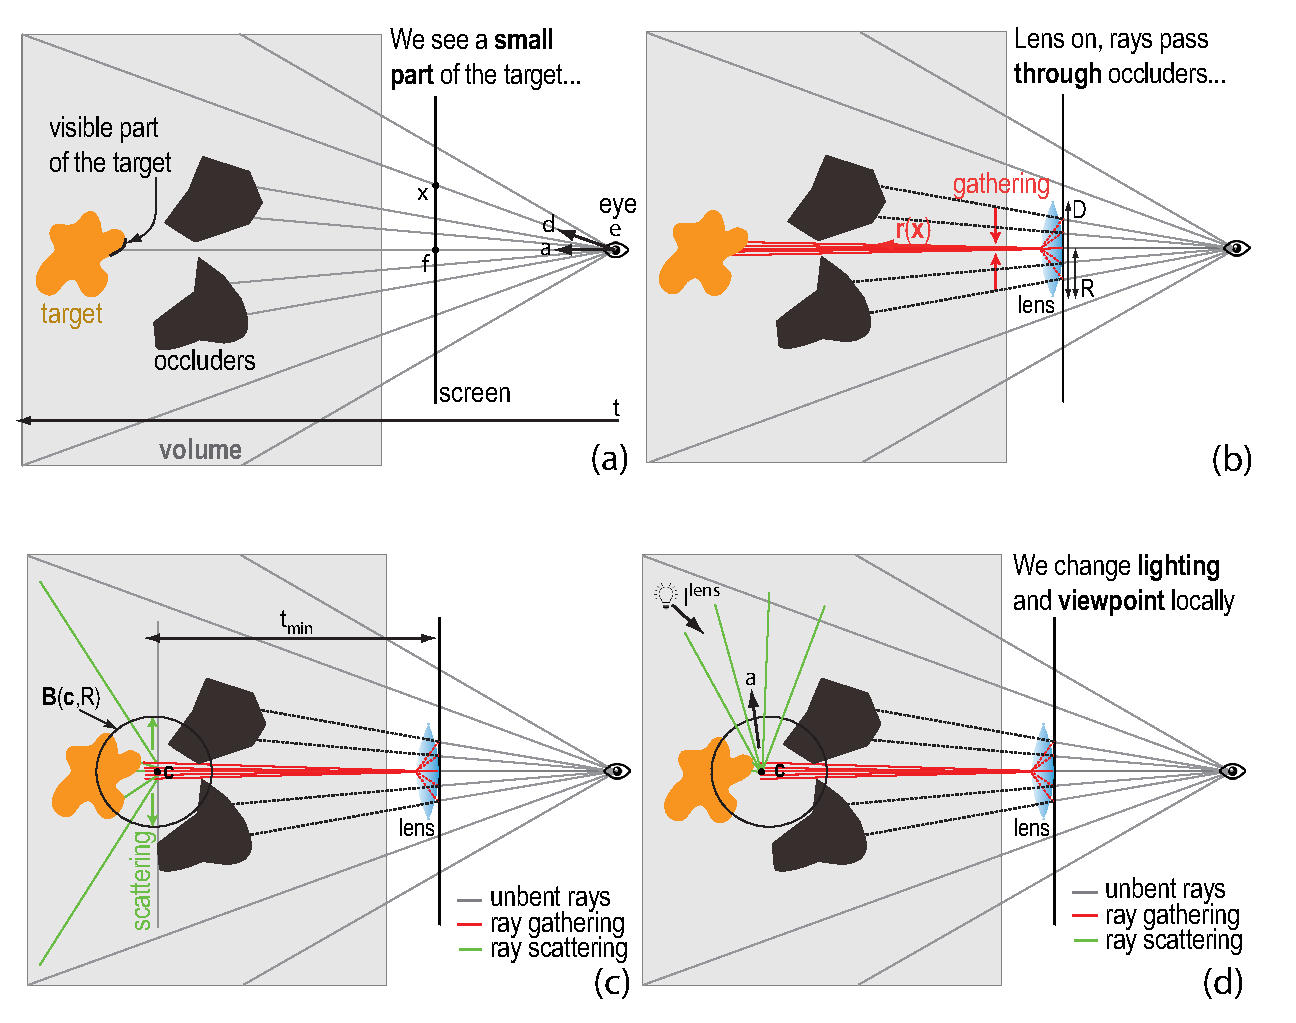
\includegraphics [width=\textwidth]{images/principle.eps}

\caption[Obstruction-free lens working.]{Obstruction-free lens working. A target is (mostly) hidden by occluders in front of it. (a) Classic DVR shows a small part of the target. (b) Our lens gathers rays to avoid occluders (\autoref{sec:gathering}). Once close to the target, rays follow again their initial paths. Yet, only a small part of the target is visible. (c) Scattering rays makes the full target visible (\autoref{sec:scattering}). Finally, we adjust the local viewing and lighting directions $\mathbf{a}$, $\mathbf{l}^{lens}$ (\autoref{sec:inter_expl}).}
\label{f:fisheye}

\end{figure}
\section{Principle}
\label{sec:principle}
%
%
Consider the typical DVR algorithm: Given a scalar volume $V \subset \mathbf{R}^3 \rightarrow \mathbf{R}$, each pixel $\mathbf{x} \in I$ in the DVR image $I \subset \mathbf{R}^2$ thereof corresponds to the compositing of sampled data along a ray that passes through $V$ and ends at $\mathbf{x}$. In classical DVR (\autoref{f:fisheye}-a), such rays are defined by the eye position $\mathbf{e}$ and a ray direction unit vector
\begin{equation}
\mathbf{d} = \frac{ (\mathbf{x} - \mathbf{e}) }{ \| \mathbf{x} - \mathbf{e} \| }
\end{equation}
. Consider now a focus point $\mathbf{f} \in I$ (the lens center) and a lens radius $R > 0$. We modify all rays passing through the lens (focus/0 area $D = \{\mathbf{x} \in I | \| \mathbf{x} - \mathbf{f} \| \leq R\}$ in order to de-occlude, magnify, and emphasize a target object. Our ray behavior is divided into three steps: (1) Provide a clear view of the target by moving closer to it and by pushing occluders aside. (2) Set a wide field-of-view (fisheye) to better see the target. (3) Modify the parameters of the lens, lighting, and opacity TF in real time to better explore the target. These steps are detailed next.

\subsection{Creating an unobstructed view}
\label{sec:gathering}
%
The scenario we address is as follows: Given a volume $V$, users produce a DVR thereof, using whatever suitable TFs and other parameters are applicable. When examining $V$ from various viewpoints, (at least) one viewpoint $(\mathbf{e},\mathbf{d})$ is found from which some intriguing structure is \emph{partially} visible in $I$. We call this structure the \emph{target}. Users next want to quickly and easily unravel the target. For this, we proceed as follows: We first \emph{gather} all rays passing through the lens pixels (focus area $D$) to follow the lens' axis vector

\begin{equation}
 \mathbf{a} = \frac{ (\mathbf{f} - \mathbf{e}) } { \| \mathbf{f} - \mathbf{e} \| }
 \end{equation}
 . As explained above, at the location $\mathbf{f}$ of the lens center, we do see an interesting partially occluded target. Hence, by definition, the gathered rays pass \emph{through} occluders to hit this target, otherwise we would not see it. We control gathering by setting the ray direction passing through $\mathbf{x} \in D$ to
%
\begin{equation}
\mathbf{r}(\mathbf{x}) = (1-\alpha) \mathbf{a} + \alpha \mathbf{d},
\label{eqn:gathering}
\end{equation}
%
with $\alpha \in [0,1]$. When $\alpha=0$ (default), all rays follow the lens axis $\mathbf{a}$, thus, can best pass through obstacles. When $\alpha=1$, rays follow a straight path. Changing $\alpha$ with the mouse wheel smoothly navigates between the lens effect, \emph{i.e.} opening up a 'hole' in the volume to see the target, and classical DVR.
%
\subsection{Setting a wide field of view}
\label{sec:scattering}
%
Once the rays pass obstacles (\autoref{sec:gathering}), we want to \emph{scatter} them so as to best sample the target. Consider that this target is at some depth $t_{target}>0$ within $V$. After the rays pass the occluders, but before they hit the target, \emph{i.e.}, travel past a distance $t_{min} < t_{target}$ through $V$, we deflect (scatter) them so as to best sample the target. For this, we set the parametric position of a ray point to
%
\begin{equation}
\mathbf{p}(\mathbf{x}, t) = \mathbf{r}(\mathbf{x})t + \beta (\mathbf{x}-\mathbf{f})(t-t_{min})
\label{eqn:scattering}
\end{equation}
%
for any pixel $\mathbf{x} \in D$ and any $t \geq t_{min}$. Here, $\beta \geq 0$, adjusted via the mouse scroll wheel while pressing the Shift key (\autoref{f:fisheye}-c), controls the ray scattering: Small values magnify a small volume area close to the ray $\mathbf{r}(\mathbf{x})$; larger values sample more of the volume behind the lens. Intuitively, this is as if we moved a magnifying lens to a depth $t_{min}$ inside $V$. Summarizing, after the user finds an interesting but partially occluded target using \emph{standard} DVR, our lens squeezes rays to pass between occluders and next fans them out to explore the target.
%
%


\subsection{Interactive exploration of the target}
\label{sec:inter_expl}
%
To achieve a more effective exploration, we can interactively modify several parameters of the DVR and the lens, as follows.
%
\begin{figure}
\centering

\includegraphics [width=\textwidth]{images/params.eps}

\caption[Changing lighting parameters in the lens.]{Changing lighting parameters in the lens. (a) Constant global specular coefficient. (b) Specular coefficient high in the lens and low outside. (c-f) Changing the in-lens light vector yields the effect of a flashlight rotating around the target. The ball icons illustrate the local light vector direction.}
\label{f:params}

\end{figure}
%



\par \textbf{Lens radius:} The radius $R$, telling how big is the 'hole' to open up in the volume to see the target, is set via the mouse wheel. The parameters $\alpha$ and $\beta$ (affecting the gathering and scattering of rays respectively) are set by the mouse wheel and modifier keys. The value $t_{min}$ (depth from which scattering starts) is set using the arrow keys.

\par  \textbf{Lens axis:} Users can rotate the lens axis $\mathbf{a}$ using a virtual trackball activated by the right mouse button. Changing $\mathbf{a}$ effectively samples the target from many viewpoints, allowing the user to look 'around' it to see parts which are not visible from the current viewpoint, but \emph{without} actually changing the viewpoint. This is of high added value, since changing the viewpoint can bring us to a view where the target is fully invisible, so we do not know where precisely to activate the lens anymore. \autoref{f:rotation} shows three such local rotations for the baggage dataset introduced in  \autoref{f:baggage_lens}. From these, we see that the star-shaped target is relatively thick.


\par  \textbf{Lighting:} We modify the volumetric Phong lighting parameters to better explore the target, as follows. Let
\begin{equation}
\mathbf{c} = \mathbf{e} + t_{min}\mathbf{a}
\end{equation} 
 be a point at depth $t_{min}$ along the lens axis, and let $B(\mathbf{c},R)$ be a sphere of radius $R$ around this point (\autoref{f:fisheye}b). We call voxels in this sphere 'in focus', and all other voxels in $V$ 'out of focus'. Let $\phi$ be the specular term coefficient, set to a high value (default: one).
First, for all voxels $\mathbf{x} \in B(\mathbf{c},R)$, we use a specular coefficient 
\begin{equation}
\phi(\mathbf{x}) = \phi (1-d)
\end{equation}
, where 
\begin{equation}
 d= \frac{\|\mathbf{x}-\mathbf{c}\|}{R}
\end{equation}. 
For all voxels outside $B(\mathbf{c},R)$, we use $\phi(\mathbf{x}) = 0$. Hence, voxels close to the focus point $\mathbf{c}$ appear highly specular; further away from $\mathbf{c}$, voxels get less specular, and voxels out of focus are purely diffuse. Secondly, we allow the user to locally rotate the light vector using the same trackball mechanism as for the lens axis rotation. Let $\mathbf{l}^{lens}$ be this vector, and let $\mathbf{l}^{global}$ be the global light vector used by standard DVR. For all voxels in focus, we use a light vector
\begin{equation}
\mathbf{l}(\mathbf{x}) = (1 - d)\mathbf{l}^{lens} + d\mathbf{l}^{global}
\end{equation}.
 
  As the user rotates $\mathbf{l}^{lens}$, the light direction will visibly change in the middle of the lens, stay constant outside it, and smoothly change in between.


\par  The above two mechanisms combined yield the effect of a moving flashlight turning around a shiny target embedded in a constantly-lit diffuse scene. \autoref{f:params} shows these mechanisms for a chest CT dataset containing a deeply buried tumor (the dataset and use-case are described in detail in \autoref{sec:chest}). We see how turning the light highlights small-scale details on the target surface (tumor) without changing the viewpoint or lens location. Moreover, the high specularity in the lens attracts the user's attention to this area; the diffuse lighting outside the lens put less emphasis on the context area. 


\par  \textbf{Opacity:} We modify the opacity transfer function along a similar idea as for lighting ( \autoref{fig:tf}). Let $TF_{o}^{global} : \mathbf{R} \rightarrow [0,1]$ be the user-chosen opacity function used globally for the volume. Let $\Gamma$ be a Gaussian pulse of unit height centered at the average density value $\bar{\rho}$ in $B(\mathbf{c},R)$ and with standard deviation $\sigma$. We estimate $\bar{\rho}$ and $\sigma$ by considering the density $\rho$ at 150 points randomly sampled inside $B(\mathbf{c},R)$. Higher values for the sample count yield visually very similar results for our tested volumes of up to $500^3$ voxels, while requiring (slightly) more computation costs. Then, for voxels in $B(\mathbf{c},R)$, we use an effective opacity transfer function   
\begin{equation}
TF_o = TF_{o}^{global} + (1-d) \Gamma
\end{equation}.
 For voxels outside $B$, we use $TF_{o}^{global}$ (standard DVR).
This is useful when the user sets $TF_{o}^{global}$ to make most out-of-lens voxels relatively transparent. In that case, $TF_o$ will still make voxels in $B$ opaque, thus allowing to see the in-focus structures better. \autoref{f:params} has been generated this way.


%ALEX: This phrase was indeed confusing, I don't know what we wanted to say with it: 
%We see here how the tumor in the lens has the same opacity as the muscle tissue outside the lens, even though the two have nearly identical densities.

\begin{figure}
\centering
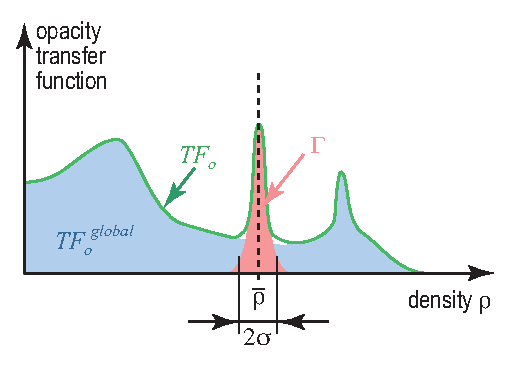
\includegraphics[width=0.95\textwidth]{images/tf.eps}

\caption{Construction of local transfer function $TF_{o}$. See \autoref{sec:inter_expl}.}

\label{fig:tf}
\end{figure}


\subsection{Smooth transitions}
\label{continuity} 
%
If we bend rays passing through the lens pixels $D$ (\autoref{eqn:gathering} and \autoref{eqn:scattering}) and trace rays starting at pixels in $I \setminus D$ as straight lines, discontinuities appear at the lens borders. We solve this as follows. Let $\mathbf{p}(\mathbf{x},t)$ be the voxels along a lens ray starting at screen pixel $\mathbf{x}$, as computed by  \autoref{eqn:scattering}. Let $\mathbf{p}^{line}(\mathbf{x},t)$ be the voxels along a straight-line ray starting at $\mathbf{x}$, \emph{i.e.}, computed using $\alpha=1$ and $\beta=0$ in  \autoref{eqn:gathering} and \autoref{eqn:scattering} respectively. For every value $t$ along every such ray, we compute the interpolated ray
\begin{equation}
\bar{\mathbf{p}}(\mathbf{x},t) = (1-f(d))\mathbf{p}(\mathbf{x},t) + f(d)\mathbf{p}^{line}(\mathbf{x},t)
\end{equation},
 where $d$ is the distance of $\mathbf{x}$ to the lens axis (normalized to unit by dividing it by $R$) and $f : [0,1] \rightarrow [0,1]$ is an interpolation function. Next, we use the rays $\bar{\mathbf{p}}(\mathbf{x},t)$ to compute the DVR by standard composition. This way, rays effectively vary smoothly from their bent versions (close to the lens axis) to straight lines (outside the lens). Setting $f(d) = d^2$ keeps the interpolation transitions close to the lens border, so most of the lens is dedicated to show the desired fish-eye effect.

\begin{figure}
\centering
\includegraphics [width=0.95\textwidth]{images/rotation.eps}

\caption{Performing local rotations in the lens allows better seeing the shape and thickness of the partially occluded target object (ninja star).}
\label{f:rotation}

\end{figure}

Separately, we use a slow-in/slow-out animation\,\cite{Dragicevic:2011:TDA:1978942.1979233} to introduce the lens effect. When activating the lens, we vary $\alpha$ and $\beta$ from their defaults ($\alpha=1$, $\beta=0$, \emph{i.e.} straight-line classical DVR) to their actual user-set values, compute the volume rendering on-the-fly, and display the resulting images. The effect resembles gradually opening a hole in the volume -- see the associated video. The speed increase at the start of the animation helps one to quickly see what is revealed in the lens; the decreasing speed at the end helps seeing where the pushed-away occluders actually go. This also gives some semantic to the moving shapes, allowing one to interpret the motion as a magnification of a target, and to keep the focus on visual entities during this transition. When deactivating the lens, we play back the animation in the opposite sense, which suggests closing the opened hole in the volume.

\section{Implementation}
\label{sec:implem}
%
We implemented our occlusion-free lens by modifying a standard DVR ray caster, publicly available in NVIDIA CUDA's SDK\,\cite{cudasdk}. We modified this ray caster to incorporate the new ray definition (\autoref{eqn:gathering} and \autoref{eqn:scattering}), the lens effect, and the local per-voxel Phong lighting parameters, all controlled via keyboard and mouse. On a PC with 16 GB RAM and a GeForce GTX TITAN X card, we achieve 15 frames per second for volumes up to $512^3$ voxels at a $1900 \times 1200$ pixels screen resolution. All in all, adding our lens to an existing ray caster should pose no significant implementation problems.

\section{Application Scenarios}
\label{sec:scenarios}
%
We next demonstrate our obstruction-free lens via five use-cases considering scalar density volumes from baggage inspection, 3D flow simulation, radiology, air traffic planning, and diffusion tensor imaging.

\subsection{Baggage inspection: An unusual blunt object}
\label{sec:baggage}
%
In airports, security agents deal with volumetric data exploration during baggage inspections. While automatic systems can detect densities of harmful substances such as C-4, TNT, and nitroglycerin, or prohibited articles (threats) like classical firearms and knives, unusual threats are hard to find. Four main concealment strategies exist\,\cite{7819413}:
\begin{itemize}
\item \textbf{Superposition}: A threat may be sheltered among dense materials. While possible to see through such a 'shield' using high penetration (enhanced X-ray power) or image processing (contrast improvement), such techniques are not universally available and also require fine-tuning many parameters, which slows down inspection.


\item \textbf{Location}: Objects located in the corners, edges, or in the luggage's frame are very hard to spot.


\item \textbf{Dissociation}: One can conceal a threat by spreading its parts in the luggage, \emph{e.g}, by disassembling a weapon and scattering its parts.

\item \textbf{Lure}: A minor threat (lure) like small scissors is clearly visible and catch the security agent's attention who can miss the real threat.

\end{itemize}


\begin{figure}
\centering
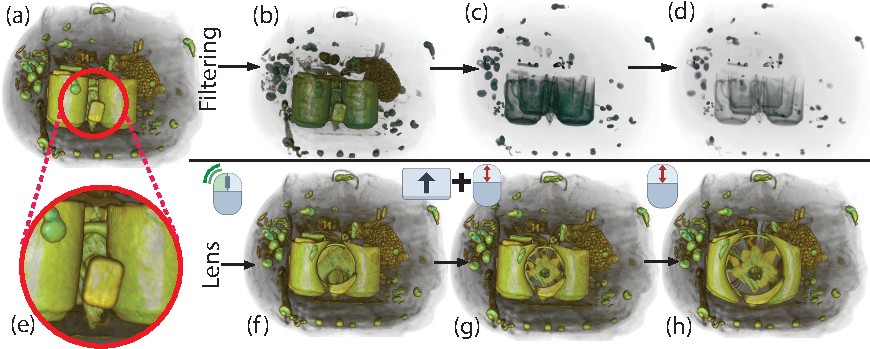
\includegraphics [width=\textwidth]{images/shuriken.eps}

\caption[Using our interactive lens on baggage.]{(a-c) A baggage scan is viewed from different angles. In view (c), a suspicious sharp object is spotted between a set of mugs. (d-f) Filtering densities using a classical 1D opacity transfer function removes progressively more of the occluders (mugs), but also the target. (g) The user applies the lens on the target object (double-click). An animation starts opening the lens, rays are gathered to pass through occluders. Halfway the animation, the object is magnified, but only the area close to the lens is visible. (h) The fish-eye field of view at the end of the animation scatters rays to fully show the target. (i) The lens is increased to magnify the target (mouse scroll).}
\label{f:baggage_lens}
\end{figure}


Baggage labeled as suspicious by human inspection or automated scan heuristics must be checked by human agents. Besides time-consuming physical unpacking, one can use 'virtual unpacking' tools that segment the 3D scan by a density-based confidence measure and next move the segmented objects away by animation to reduce occlusion\,\cite{Li:2012:LVV:2425296.2425325}. Such systems have been patented and used in production\,\cite{patent}. However, when the automatic segmentation is not optimal, the user must manually change its parameters, repeat the segmentation and animation, which goes back to being time-consuming.

Consider the baggage scan in \autoref{f:baggage_lens} ($283 \times 189 \times 344$ voxels, dataset obtained from an actual airport scan). Automatic baggage inspection systems will not detect anything suspect here. However, while visually exploring this baggage from different angles (\autoref{f:baggage_lens}a-c), we see an object hidden between a set of mugs. To reduce occlusion, a common solution in baggage inspection is to filter materials by density in order to show or hide subsets of the volume. However, for our dataset, the suspect target has almost the same density as the surrounding mugs, so removing the latter also removes the target (\autoref{f:baggage_lens}d-f). Using the obstruction-free fish-eye lens helps here: Clicking on the sharp detail visible in \autoref{f:baggage_lens}c first gathers rays so they pass through the low-density zone between the mugs (\autoref{f:baggage_lens}f). The animation that opens the lens 
(\autoref{f:baggage_lens}e-g) reveals an unobstructed view of the target. However, this shows only a small part of the target. Scattering rays next fully reveals the target (\autoref{f:baggage_lens}h). Adjusting the lens size shows a more detailed view of the target (\autoref{f:baggage_lens}i). Next, locally turning the viewpoint around the target (\autoref{f:rotation}) allows the agent to decide that the target is a shuriken (Japanese ninja star weapon). Since the object is very thick and blunt (see \autoref{f:rotation}), it is not an actual weapon, thus not a threat.

We evaluated our lens for this use-case by a user study. This evaluation is described bellow in \autoref{questanswers}.

\subsubsection{Early results}
\label{questanswers}

Eight airport security specialists were recruited (ages 23 to 43; experience in baggage scanning 8 months to 20 years; average familiarity with 3D tools, none considering him/herself an expert.


All attended a 20-minute global demo of the lens operation. Next, they were given each a personal training session for using the tool (5 minutes), in which they were instructed on the mouse and keyboard controls. After this, they were asked to work in pairs to examine the above-mentioned baggage CT dataset to form a decision on the nature of the ninja star possible threat (20 minutes of tool usage per person, after which the pair was changed). The idea behind this is that one person operates the tool while the other poses questions or suggest explorations, much like typical airport security operators work with a scanner. In the end, they all separately filled in a web questionnaire covering several questions and also provided open feedback (questionnaire available in the \autoref{AppendixA}). 


\autoref{questanswers} shows the answers. The first question-set (S1) regarded how easy-to-use, generally effective, and effective \emph{vs} other known tools our lens is for \emph{untargeted} inspection, \emph{i.e.}, when no suspect target is partially visible. Here and next, other tools denote classical 2D X-ray or 3D CT scans used in baggage scanning that the subjects know. As \autoref{fig:graph3}, \autoref{fig:graph4}, and \autoref{fig:graph5} show, 
the answers (on a 5-point Likert scale) were predominantly positive: The tool is easy to use, is useful, and is actually more useful than known tools for untargeted exploration. The second question-set (S2) regarded how good our tool is to examine \emph{specific} targets which are partially visible. Here again, the answers were predominantly positive (\autoref{fig:graph6}, \autoref{fig:graph7}, and \autoref{fig:graph8}). The main appreciated features of our tool are listed in \autoref{fig:graph9}.





\begin{figure}
\centering
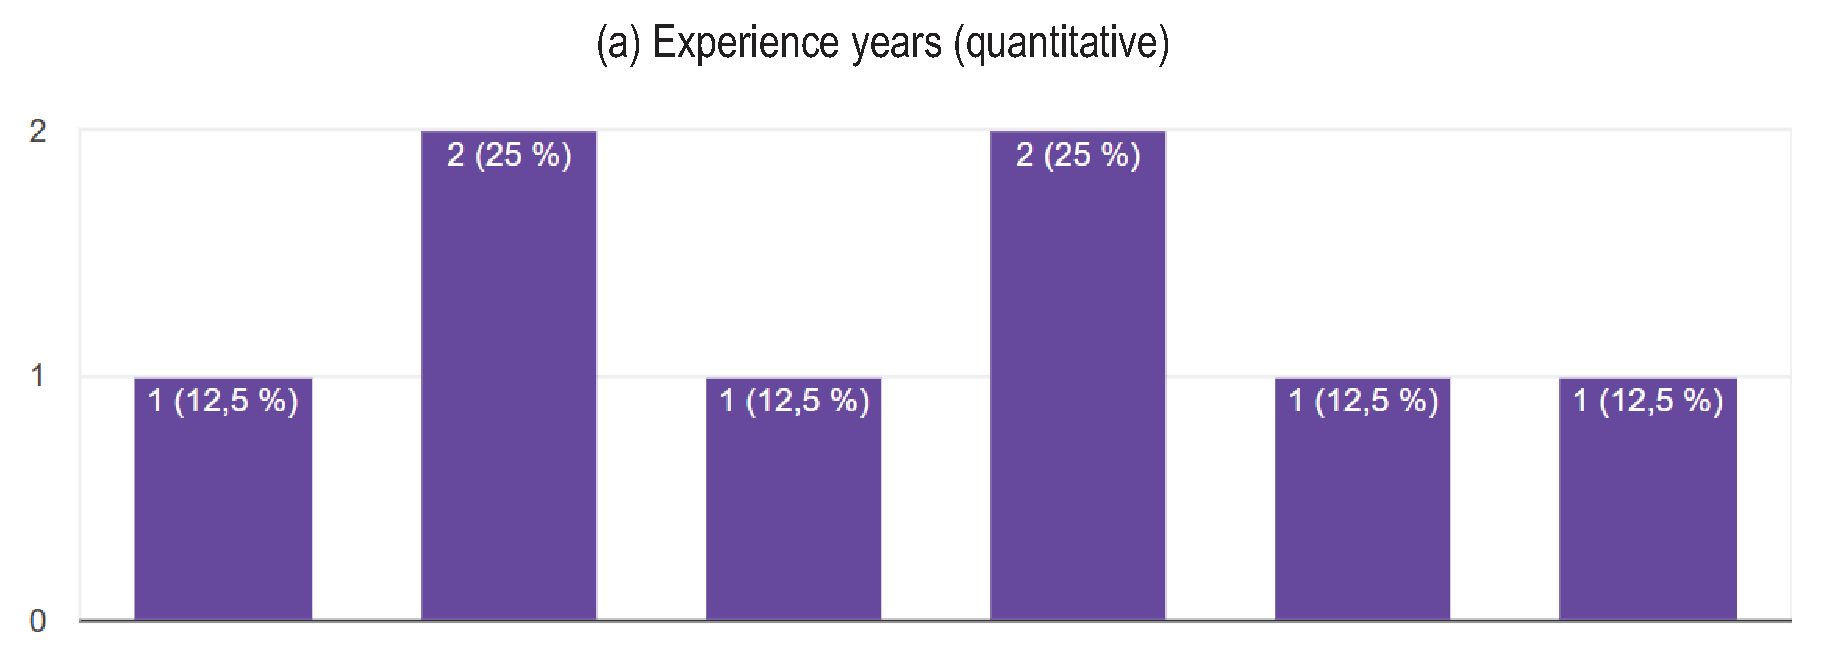
\includegraphics [width=\textwidth]{images/graph1.eps}
\caption{Evaluation of lens-based baggage inspection (\autoref{sec:baggage}): Experience years.}
\label{fig:graph1}

\end{figure}


\begin{figure}
\centering
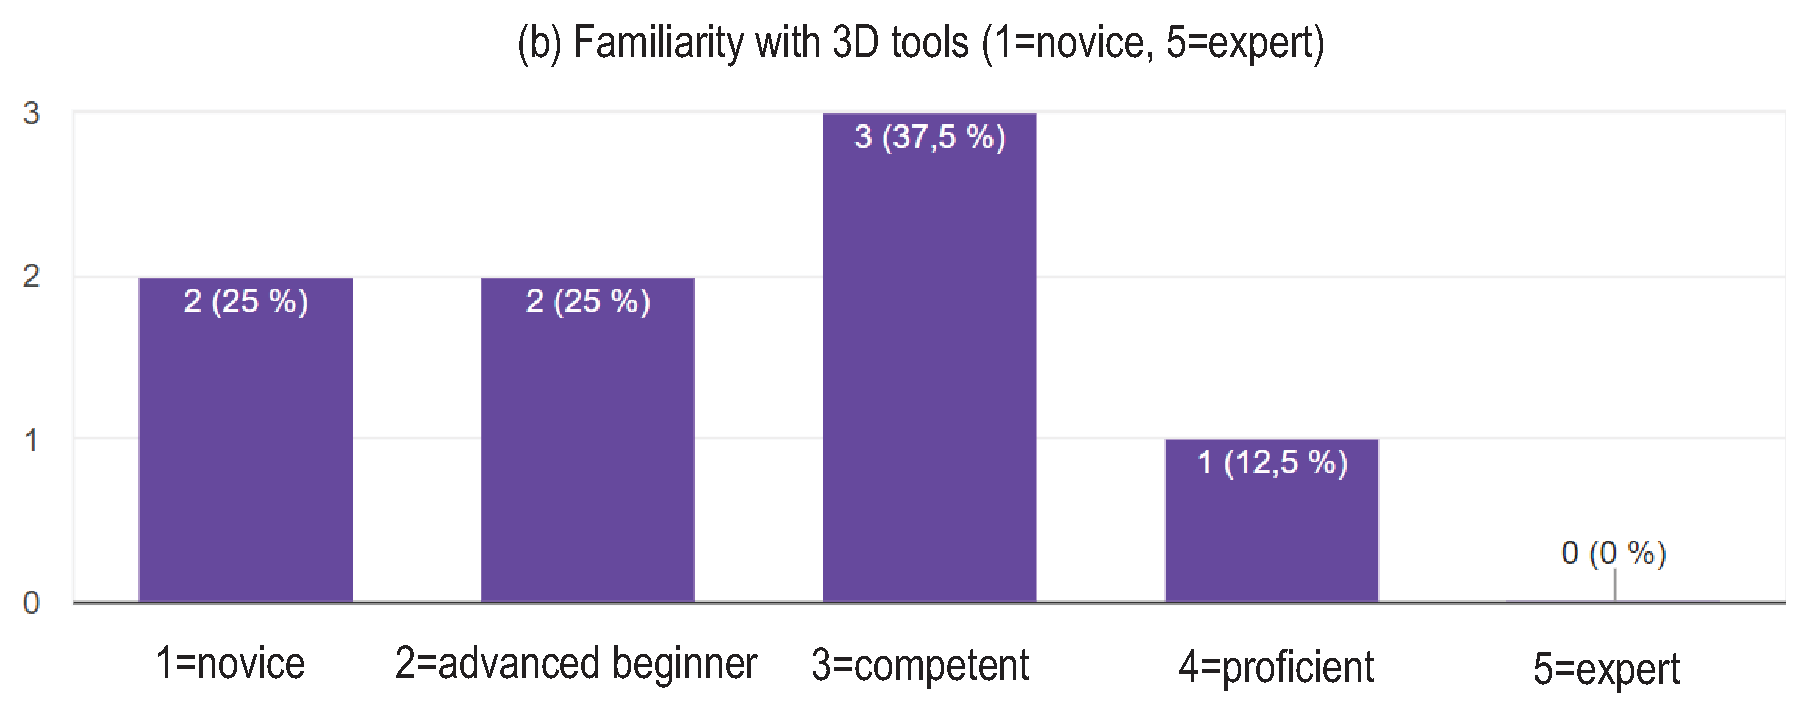
\includegraphics [width=\textwidth]{images/graph2.eps}
\caption{Evaluation of lens-based baggage inspection (\autoref{sec:baggage}): Familiarity with 3D tools.}
\label{fig:graph2}
\end{figure}


\begin{figure}
\centering
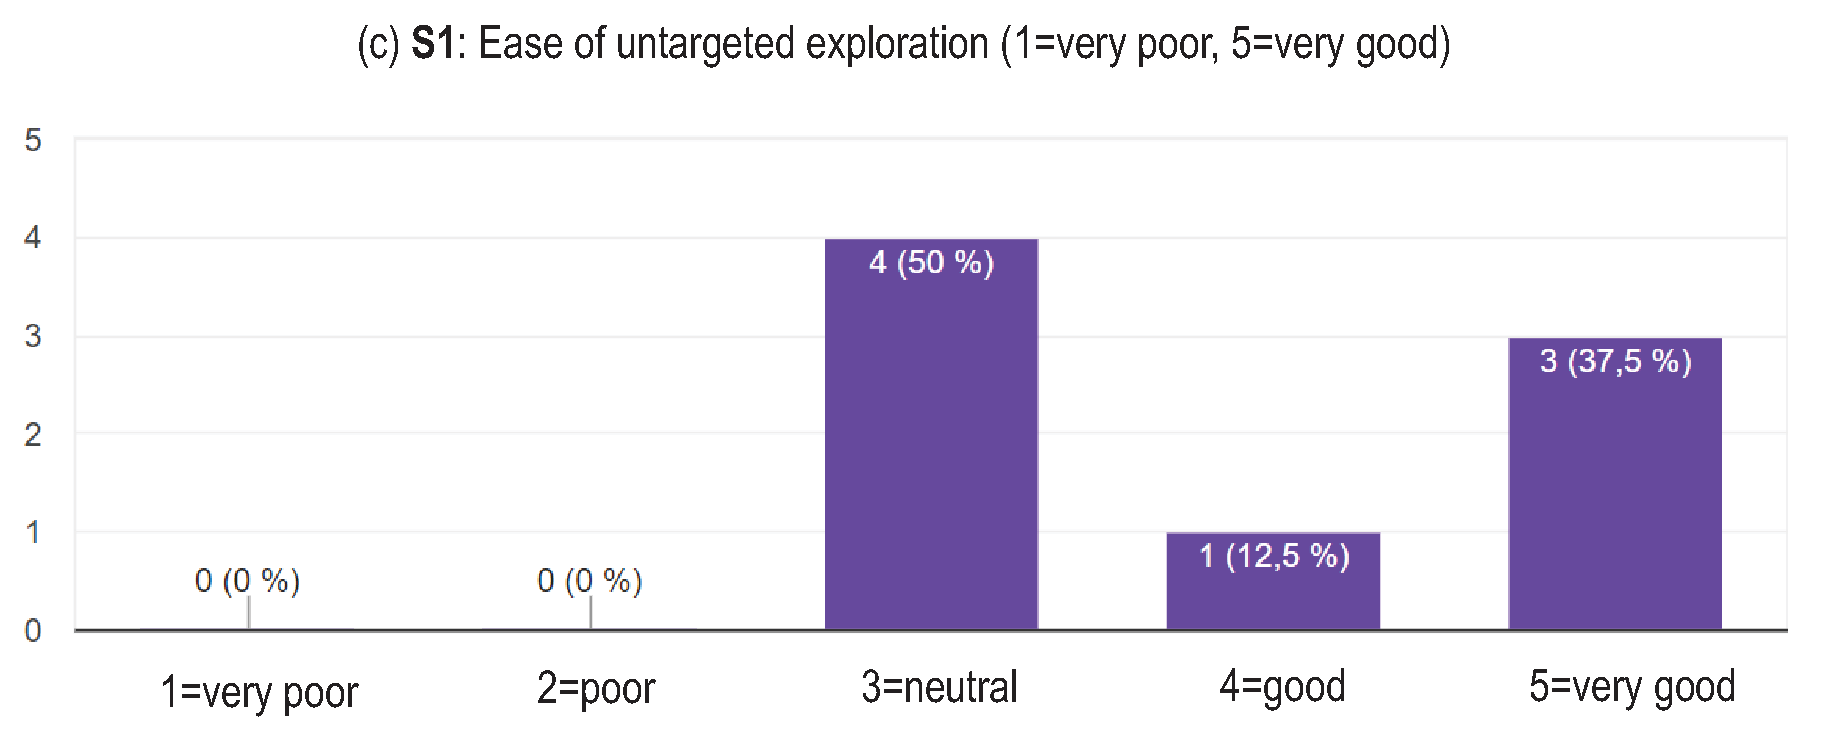
\includegraphics [width=\textwidth]{images/graph3.eps}
\caption{Evaluation of lens-based baggage inspection (\autoref{sec:baggage}): Scenario 1 - Ease of untargeted exploration.}
\label{fig:graph3}
\end{figure}


\begin{figure}
\centering
\includegraphics [width=\textwidth]{images/graph4.eps}
\caption{Evaluation of lens-based baggage inspection (\autoref{sec:baggage}): Scenario 1 - Tool's value for untargeted exploration.}
\label{fig:graph4}
\end{figure}

\begin{figure}
\centering
\includegraphics [width=\textwidth]{images/graph5.eps}
\caption{Evaluation of lens-based baggage inspection (\autoref{sec:baggage}): Scenario 1 - Tool's value, untargeted exploration, vs other used tools.}
\label{fig:graph5}
\end{figure}

\begin{figure}
\centering
\includegraphics [width=\textwidth]{images/graph6.eps}
\caption{Evaluation of lens-based baggage inspection (\autoref{sec:baggage}) : Scenario 2 - Ease of untargeted exploration.}
\label{fig:graph6}
\end{figure}

\begin{figure}
\centering
\includegraphics [width=\textwidth]{images/graph7.eps}
\caption{Evaluation of lens-based baggage inspection (\autoref{sec:baggage}): Scenario 2 - Tool's value for untargeted exploration.}
\label{fig:graph7}
\end{figure}

\begin{figure}
\centering
\includegraphics [width=\textwidth]{images/graph8.eps}
\caption{Evaluation of lens-based baggage inspection (\autoref{sec:baggage}): Scenario 2 - Tool's value, untargeted exploration, vs other used tools.}
\label{fig:graph8}
\end{figure}


\begin{figure}
\centering
\includegraphics [width=\textwidth]{images/graph9.eps}
\caption{Evaluation of lens-based baggage inspection (\autoref{sec:baggage}): Which functions of this tool bring the most added-value vs tool you already know and have used for the same task (categorical).}
\label{fig:graph9}
\end{figure}


We next summarize the received open feedback. According to the subjects, our tool can provide them a better perception of the items inside the baggage as compared to the classical 2D single-viewpoint X-ray machinery they routinely use. Quotes from the open feedback: ''clear added-value compared to all systems I know''; ''this tool is a real gain for examining luggage with uniform and/or high densities''; ''definitely better than known tools for examining threats I am not familiar with / I have not seen before''. However, our tool should not be used for the typical carry-on baggage inspection which has a very small allowed inspection time (15 to 20 seconds). Our tool is much more interesting for inspecting checked-in baggage, where inspection time-windows are up to 3 minutes. The perceived added value for this use-case is also higher: Opening up checked-in baggage for manual inspection is much more complicated and time-consuming than for carry-on baggage. Moreover, the only system for inspecting checked-in baggage that the subjects knew of is a scanner that aims to \emph{automatically} detect threats via X-ray imagery; this system suffers from false positives, so a manual examination tool like ours could quickly eliminate such false positives, and thus the delays of opening up checked-in baggage. Finally, several subjects suggested that adding a function to display a classical 2D slice view (activated by a key press and aligned with the focal point) would be useful since this would show additional detail.


\subsection{Fluid flow: A deep-buried spherical vortex}
\label{sec:flow}
%
%
Flow visualization using streamlines has a long history\,\cite{brambilla2012illustrative,merzkirch2012flow}. For 3D datasets, a key challenge is to balance the streamline density. Low values allow seeing inner regions in the data but can subsample (miss) patterns. High values show more data but create too much occlusion. We next show how our lens can be used to alleviate problems in the latter case. The dataset\,\cite{griebel2004flow} captures the simulation of water flow in a basin computed on a grid of $128 \times 85 \times 42$ cells using 4595 streamlines with 183K sample points traced by pseudo-random seeding. We convert this set of 3D curves (polylines) to a scalar volume by using GPU-accelerated kernel density estimation (KDE)\,\cite{lhuillier2017ffteb}. Similar techniques have been used to compute density maps of 2D trail-sets\,\cite{hurter2012graph,cubu,hurter2015image}. 

We first explore the density volume ($500^3$ voxels) using standard DVR (\autoref{f:stream_lens}). Note that, given KDE's smoothing effect, streamlines appear as finite-thickness tubes rather than pixel-thin curves. After turning the viewpoint a bit, we notice a dense spherical item deep in the data (\autoref{f:stream_lens}a). To see its shape better, we increase opacity; however, this immediately increases occlusion so the item becomes invisible. Conversely, decreasing opacity to reduce occlusion makes the item almost transparent. Our lens solves the problem: In the initial view (\autoref{f:stream_lens}a), we point at the target and turn on the lens. This pushes away the occluding stream bundles, and shows that our item is a set of densely-packed, low-speed, tightly-turning streamlines that create a ball-like vortex (\autoref{f:stream_lens}b). 
To make sure our target is spherical, we view it in the lens from different directions, by interactively changing the ray directions in the lens (\autoref{f:stream_lens}c). Finally, we can close the lens but keep the target magnified (\autoref{f:stream_lens}d).
Finding the details of this vortex cannot be done using standard DVR. Interestingly, this vortex has also not been discovered by any of the visualization techniques that used this dataset (according to our knowledge) \,\cite{telea_vis_99,griebel2004flow,ddh,lhuillier2017ffteb}. 

\begin{figure}
\centering
\includegraphics [width=\textwidth]{images/stream_lens.eps}

\caption[Flow volume exploration with two different opacity transfer functions (top and bottom rows).]{Flow volume exploration with two different opacity transfer functions (top and bottom rows). In viewpoint (a), we notice a small high-density spherical item. (b) We apply the lens at that location (double click). (c) The directions of rays in the lens are changed to see the whole target in the lens (right click + mouse drag change direction). (d) The lens is gradually closed while keeping the focus area magnified (shift + scroll).}

\label{f:stream_lens}
\end{figure}

\subsection{Chest scan: A hard to see tumor}
\label{sec:chest}
%
In our third use-case, we consider a contrast chest CT scan ($512 \times 512 \times 110$ voxels) of an elderly patient with a sizeable lung tumor. The tumor was detected in a CT scan performed after the patient reported acute chest pain. Typical examination of these scans by the pulmonologist and radiologist in charge involves slice-based views. \autoref{f:slicer}a-c and \autoref{f:slicer}d-f show two such slice sets (axial, coronal, and sagittal views), produced using typical lung, respectively mediastinal, contrast presets.

 Although the tumor is visible in all these views, its exact shape, morphology, and connection to the lung walls are hard to assess. Finding such details on the tumor is essential, explained the doctors in charge, to determine the TNM score\,\cite{brierley} and also planning treatment. Using standard DVR makes the tumor and its 3D position partially visible (\autoref{f:slicer}f). Yet, occlusion from the rib cage and other tissues is still present. Using both TF presets and manually changing the TFs in the 3D Slicer tool\,\cite{slicer} used to create the DVR could not help de-occluding the tumor without making it partly transparent.
 
  The slice images in \autoref{f:slicer}a-f confirm this by showing that the gray values for the tumor and surrounding skin-and-muscle tissue are very similar. This is due to the fact that the tumor had grown rapidly and started necrotizing, which filled it with fluids, making its density very similar to that of the obstructing (skin and muscle) tissue, explained the pulmonologist. Hence, one cannot remove such occluding tissue in a classical DVR setting by opacity TF manipulation without also removing the tumor. This makes examining this specific tumor harder than for regular cases.

\begin{figure}
\centering
\includegraphics [width=\textwidth]{images/slicer.eps}
\caption[Lung tumor visualization using slices and standard DVR.]{Lung tumor visualization using slices (a-c) and standard DVR (d). Annotations are manually added by the examiner to delineate the tumor location. Images constructed using the 3D Slicer tool\,\cite{slicer}.}
\label{f:slicer}
\end{figure}

We next used our lens to examine the tumor. \autoref{f:params} shows several sample snapshots. We see that the tumor is significantly more visible when using the lens than when using standard DVR (\autoref{f:slicer}d), both in terms of removing the occluding tissue and in terms of the tumor's opacity -- compare the inset in \autoref{f:slicer}d with the images in \autoref{f:params}. Secondly, relighting the tumor from various directions allows one to see small-scale morphological details such as the tumor's surface shape and its connection via protuberances and veins with the lung walls.

We asked the two medical specialists (pulmonologist and radiologist) in charge to state the potential advantages and/or limitations of our lens as compared to standard slicing and DVR techniques, after a 20-minute usage of the tool. 
Both specialists have over 10 years of medical experience in treating lung cancer, and routinely use several slicing and DVR tools. They work in a private hospital in Belgium and are not actively associated with medical imaging research. Our identities were hidden from them during the lens evaluation. The provided input can be summarized as follows: The occlusion-free lens is definitely easier and faster to use than classical DVR and/or slicing techniques. It is especially more effective than these to get a quick, first impression of a deep buried anatomical detail. Changing the lens' parameters by direct interaction is as simple as changing window/level functions in a typical slice-based tool, and is definitely simpler than tuning typical DVR parameters to obtain similar results. This 'entices' the user to explore, which is a good aspect. The fact that the lens minimizes viewpoint change (volume rotation), \emph{i.e.}, after a suitable viewpoint was found from which a (small) part of the target is visible, one doesn't need to change this viewpoint, is a strong feature, as 3D viewpoint changes are disruptive and cost time. This is important in a cost-aware environment where specialists have very limited time (about 20 minutes) to assess a CT scan. However, the lens should not \emph{replace} classical slice-based exploration, which shows small-scale details better. In the context of the current dataset (\autoref{f:slicer}), the lens was useful to both confirm the TNM score (T3 grade tumor, 6.5 cm in size) found via the 2D slices, but much more so for understanding how and where the tumor is connected to surrounding tissue, which is very hard to do using only 2D slices.

\begin{figure}
\centering
\includegraphics [width=\textwidth]{images/aircraft.pdf}

\caption[Visualizing one day of aircraft trajectories over France.]{Visualizing one day of aircraft trajectories over France\,\cite{hurter2009fromdady}. (a) Overview of all trails. (b) Zoom, filtering, and color mapping techniques are used to highlight an outlier trajectory of an aircraft performing an eight-shaped loop. Revealing this outlier costs significant user effort.}
\label{f:fromdady}

\end{figure}


\subsection{Aircraft trajectories: Outliers in the French sky}
\label{sec:atc}
%
%
We next consider a task from air traffic planning -- detecting and studying outliers in large-scale datasets containing tens of thousands of 3D (latitude, longitude, height) trails of aircraft over a given spatio-temporal region\,\cite{hurter2014interactive}. Such datasets are typically viewed using 2D (latitude, longitude) plots where opacity encodes the spatial density of flights -- see \autoref{f:fromdady}a, which shows one day of recorded aircraft trajectories over the French airspace. \autoref{f:fromdady}(b) shows a detail zoom-in, where we can see an abnormal -- that is, far from straight or slightly curved -- aircraft trail: A tanker aircraft performed an eight-shaped loop as it was waiting to refuel other aircraft. Revealing such patterns using 2D techniques, \emph{e.g.} \cite{hurter2009fromdady}, is very hard. In particular, it is hard to de-occlude these patterns from the overall context of criss-crossing aircraft trails, even when one knows their 2D spatial location.

Our lens can help with this task, as follows. We first convert the set of 3D trails to a $500^3$ density volume, using KDE as for the streamline use-case (\autoref{sec:flow}). Examining this volume via standard DVR shows an outlier trail at some point in space, see curved patterns in \autoref{f:aircraft_lens}a. Activating the lens on this area and interactively tuning the target depth $t_{min}$ (since we don't know the trail's height) beings the outlier trajectory in focus and pushes away occluding trails (\autoref{f:aircraft_lens}a). Like in the other examples presented so far, we can quickly change the magnification factor and view direction to better study this trail in context (\autoref{f:aircraft_lens}b-d). From these images, we easily see that the outlier trail has an eight shape. Revealing this outlier trail using standard 2D visualization techniques\,\cite{hurter2009fromdady} costs several minutes. Doing the same using our lens costs under one minute. Also, comparing \autoref{f:fromdady}b and \autoref{f:aircraft_lens}b-d, we argue that the eight-shape of the outlier trail is much more prominent, and thus recognizable, in the latter images (made using our lens) than in the former ones. Last but not least, the 3D DVR approach that our lens enhances explicitly encodes flight height information, so our lens can use it by interactively tuning the depth value $t_{min}$ where the lens is focused. This cannot be done with 2D techniques which ignore the depth dimension.

We validated our findings with an air traffic data scientist with more than 10-year experience in air traffic control and planning. She confirmed that this specific eight-shape trail in \autoref{f:fromdady}(b) is an actual aircraft which performed waiting loops and acted as a fuel supplier for military aircraft. Other comments included the following: Compared to standard 2D visualization techniques, our tool makes detecting outliers easy since there is no need for complex manipulation to reveal such outlier trails. Also, the user does not have to deal with color and alpha mapping parameter-tuning to make specific outliers emerge. Separately, trail visualization easily creates many occlusions leading to either fully opaque areas or too much local overlap, which both hinder seeing and examining specific trails. Our lens does help such cases by distorting the space to locally remove such occlusions. All in all, in the studied dataset (\autoref{f:fromdady}), the lens was specifically useful since, for high transparency, one would not detect the outlier trail, while for low transparency, one would get a hint of the outlier's existence, but not see it in detail due to too much occlusion; the lens allows using low transparency, but removes the clutter caused by it to reveal the outlier.


\begin{figure}
\centering
\includegraphics [width= \textwidth]{images/aircraft_lens.pdf}
\caption[Inspecting an abnormal aircraft trail.]{Inspecting an abnormal aircraft trail. (a) The abnormal trail is spotted in an all-trails view as it is highly curved while all other trails are relatively straight. Activating the lens at the outlier location (b) and changing the magnification factor (c) reveals the trail's eight-shape. (d) Rotating the viewpoint provides spatial insight on the embedding of the outlier in the surrounding trails.}
\label{f:aircraft_lens}
\end{figure}
%

\subsection{Brain fibers: Uncluttering the bridge}
\label{sec:dti}
%
Our last use-case considers the exploration of fiber tracts visualized as streamlines of the major eigenvector of a diffusion tensor imaging (DTI) field. Such datasets have a spatially complex structure which makes them hard to explore\,\cite{assaf08}. In particular, fiber tracts are spread volumetrically over the entire extent of the brain, and create tangled patterns inside which it is hard to see much. DVR techniques are often used to render such tracts, one of the advantages being that close fibers get visually 'merged' to reveal spatially coherent structures, an effect which is not possible when fibers are rendered as polylines. However, DVR methods also create more occlusion, thus difficulties in seeing structures deep within the volume.

We consider an $128 \times 128 \times 51$ DTI volume (same dataset as in\,\cite{everts15}). We traced 150352 fibers seeded in, and going over, regions of high fractional anisotropy in this volume. We filtered out fibers shorter than 2mm, yielding a total of 120593 fibers to display (6.4M sample points). Next, we converted this fiber-set to a $512^3$ density volume, using KDE with a 3D isotropic kernel of radius 15 voxels, like for the streamline use-case (\autoref{sec:flow}). \autoref{fig:dti}a shows the result, rendered with DVR, with opacity function mapping the fiber density. While terminal fibers are well visible, we cannot see anything inside the volume. Activating the lens in the middle of the volume opens a hole through which a small part of the \emph{corpus callosum}, the fiber bundle wrapping the bridge that connects the two hemispheres, becomes visible. By slightly decreasing opacity (\autoref{fig:dti}c), the \emph{corpus callosum} gets clearly visible, appearing as a compact structure, due to the KDE blending of neighbor fibers. Obtaining such a view of the \emph{corpus callosum} only using DVR would be very hard, since transfer functions would either render separated (non-merged) fibers, or else make the fibers surrounding the structure of interest too thick and occluding. 

This scenario has the main difference compared to all previous ones. In all earlier cases, the standard DVR of the data (that is, without the lens) showed us a partial small cue of the structure of interest within the volume, and we used the screen-space location of this structure as the focus point where to activate the lens. In this last scenario, there is no point in the original DVR image (\autoref{fig:dti}a) from which the \emph{corpus callosum} is even partially visible, due to the high opacity given by the used transfer function. Hence, the user can activate the lens at \emph{any} desired point to peek inside, and towards the center of, the volume. Given the nature of the data, the structure of interest is quite easily visible from most such viewpoints (see lens inset in \autoref{fig:dti}b). Once its presence is revealed, the user can next adjust the viewpoint and/or the opacity transfer function to get an optimal view on the target, such as the one shown in \autoref{fig:dti}c. Summarizing, we can use our lens also in cases when no partial view of a target is available. 

\begin{figure}
\centering
\includegraphics [width=0.8\textwidth]{images/dti.eps}
\caption{Revealing the \emph{corpus callosum} in a DVR of a set of DTI tracts.}
\label{fig:dti}
\end{figure}

%
\section{Discussion}
\label{sec:discussion}
%
%
Several points of our lens proposal are worth discussing, as follows.


\par \textbf{Lens activation:} Our lens can support two types of explorations. First, when the user perceives a \emph{part} of a target of interest in a classical DVR image, the lens can be used to reveal the target in full detail. This \emph{directed} exploration supports the task `show me more information about \emph{this} item'. The use-cases in \autoref{sec:baggage}-\autoref{sec:atc} are of this type. Secondly, the user can open up a DVR volume at a 2D location from which no partial detail is visible. This is useful when we know that there \emph{is} an interesting target buried in the volume even without seeing it (\emph{corpus callosum} use-case in \autoref{sec:dti}), thus supports the task `show me the data I \emph{know} it is somewhere in there', or for free exploration to find unknown patterns in a volume, \emph{i.e.} for the task `show me what this volume \emph{may} hide in it'. In the first exploration type (target not fully occluded), our lens is simple and rapid to use -- point, click, and optionally rotate light or viewpoint. In the second exploration type (target fully occluded or not even sure whether an interesting target exists in the data), the lens is equally simple to use, but several tries to select a suitable focus point and lens depth are needed.

\par \textbf{Lens shape:} Occluders are pushed away, and deformed, isotropically (\autoref{sec:scattering}, \autoref{continuity}). This simple lens model requires a single parameter, the lens radius $R$, which makes its usage easy. The deformations evolve smoothly from the lens center (maximal) to outside the lens (no deformation), see \autoref{continuity}, which effectively blends the local (in lens) focus with the global (out of lens) context (R3). However, this strongly compresses the deformed occluders close to the lens border, making them hardly visible when the lens is fully active. A possible refinement would be to reduce the deformation of the pushed-away occluders while still pushing them away, thereby improving the F+C effect (R3). However, this would occlude areas outside the lens, basically moving occlusion from \emph{inside} the lens to \emph{outside} and close to it. Finding an optimal balance between minimal deformation (so one can recognize the pushed-away occluders) and minimal clutter (so these occluders do not destroy the lens context) is a topic for future work. Separately, deformed rays may intersect with straight rays, thereby sampling the same voxel(s) to different image pixels. We did not observe in our usage any artifacts that can be ascribed to this issue, nor did the other users of our tool. This can be explained by the fact that such ray intersections are relatively few and we use a compositing transfer function, akin to a low-pass filter.


\par \textbf{Parameter setting:} Our lens depends on several parameters: the 2D lens center $\mathbf{f}$, lens radius $R$, lens axis direction $\mathbf{a}$, local light direction $\mathbf{l}^{lens}$, scattering start-distance $t_{min}$, and gathering and scattering parameters $\alpha$ and $\beta$. All these parameters are controlled via a mouse-driven virtual trackball, key modifiers, and the arrow keys (\autoref{sec:principle}). As the lens works at 15 frames per second, the user can quickly tune the parameters and see their effect (R1). Moreover, all parameters start with good preset values (\autoref{sec:principle}). A possible refinement would be to pre-segment the target, based on user-given values for $\mathbf{f}$, $R$, and $t_{min}$, thereby determining $\beta$ automatically. However, we believe that manual control of the scattering $\beta$ is important to allow users to choose their most suitable field-of-view angle. In fact, this flexibility allows a better exploration of the local context (R2).


\par \textbf{Implementation:} We implement our lens by modifying the ray trajectories constructed in the inner loop (per-pixel raycasting) of a public DVR raycaster\,\cite{cudasdk}. Apart from this, we change the per-voxel lighting and transfer function based on the voxel location in the lens and the parameters given by user interaction (\autoref{sec:inter_expl}). Such changes are limited and easily applicable to any (parallel) raycaster.


\par \textbf{Limitations:} As explained, de-occluding a target requires either a small fragment thereof to be visible (if so, de-occlusion is very simple and fast), or requires the user to choose the lens focus and target depth based on other insights (which, as explained, requires more trial-and-error). At a higher level, many lens mechanisms exist in the literature, as discussed in \autoref{sec:requirements}. While we have argued that, to our knowledge, none of them simultaneously supports requirements R1,$\ldots$,R4, comparing such mechanisms with our lens for specific use-cases and datasets is an important test for the \emph{end-to-end} effectiveness of our proposal. We have not covered this point as obtaining (or replicating)  implementations of such lenses is very challenging. This remains an important open point for future work -- both for our proposal but also for all other volumetric lens proposals in the literature. In particular, none of the techniques in \autoref{tab:methods} were compared side-by-side against other techniques. We have performed three user evaluations involving specialists in airport baggage security (\autoref{sec:baggage}), pulmonology (\autoref{sec:chest}), and air traffic control (\autoref{sec:atc}). In all cases, users were not involved in this work, nor with other work of the authors. However, the set-up of these evaluations stays at the level of formative user experiments. To confirm and refine the obtained (positive) findings, more formal user studies are needed, which we plan to cover next.

\section{Conclusions}
\label{sec:conclusions}
%
In this chapter, we presented a new fish-eye-like context-and-focus lens that addresses the occlusion problems inherent in scalar volume rendering. The principle of our lens consists in first gathering (squeezing) rays so that they easily pass through occluding densities (given a user-specified opacity transfer function) and next scattering (fanning out) rays to best sample the target of interest. Our lens can be directly applied to any DVR raycaster and scalar volume dataset. Its main constraint is that the user should be able to find a viewpoint from which the target of interest, deep buried in the data, is at least slightly visible. We also present several modifications of the local rendering parameters within the lens (view direction, lighting parameters, opacity transfer function) that aim to both better separate the focus (lens) from the context (volume) and also allow more detailed examining of the target. Our lens is easy to use -- all its parameters are controlled via direct mouse-and-keyboard interaction -- and can be efficiently implemented atop of a standard GPU ray caster. Our lens is especially useful for highlighting structures of interest which are both deeply embedded in volumetric data and cannot be revealed by standard transfer function manipulations due to similar densities in the occluders and target. We demonstrate these points using five use-cases involving datasets from baggage detection, fluid visualization, air traffic control, and chest radiology, and DTI fiber tracts.

Several improvements to our proposal are possible, as follows. First and foremost, heuristics can be sought to link all our free parameters (lens size, focus depth, interpolation between focus and context) directly to the volume data, so the user interaction is minimized and therefore exploration efficiency is increased. Secondly, our lens could be extended to different types of volumetric datasets, such as multivariate (vector, tensor) fields. Last but not least, a formal wider-scale evaluation of how the lens addresses more specific tasks, and how it compares to existing tools for these tasks, such as other lens types, is a goal we aim to pursue next.
\chapter{Volume rendering on mobile devices (Virtual Reality, Augmented Reality, Mixed Reality) }
\label{mixedReality}

This chapter presents the research I have started at the end of this thesis. 
We address the volume rendering challenges on mobile devices (Virtual reality, augmented reality, and mixed reality). Mobile devices are getting more and more popular across the population. Although their technical specifications can be totally different from one device to another, they are all becoming more powerful int terms of memory, CPU, GPU, and features.

\section{Introduction}

First of all, let us define and be more following terms: virtual reality, augmented reality, and mixed reality.

\par \textbf{ Virtual Reality (VR)} immerses users in a fully artificial digital environment. In fact, This technology immerses users in a completely virtual environment that is generated by a computer. The most advanced VR experiences even provide freedom of movement – users can move in a digital environment and hear sounds. Moreover, special hand controllers can be used to enhance  virtual reality experiences.\newline
You need to wear a special VR headset to experience virtual reality. Most VR headsets are connected to a computer (Oculus Rift) or a gaming console (PlayStation VR) but there are standalone devices (Google Cardboard is among the most popular) as well. Most standalone VR headsets work in combination with smartphones: the user insert a smartphone into a headset, then wear this headset, and immerse in the virtual reality.

\par \textbf{Augmented Reality (AR)} allows users to see and interact with the real world while digital content is added to it. As a popular example, we can think of Pokemon Go which causes millions of people all over the world have been rushing with their smartphones in search for small virtual creatures. That is the most pertinent example of augmented reality. \newline
If you own a modern smartphone, you can easily download an AR app and try this technology. There is a different way to experience augmented reality, though  with special AR headsets, such as Google Glass, where digital content is displayed on a tiny screen in front of a user's eye.

\par \textbf{Mixed Reality (MR)} is the most recent development in reality technologies that sometimes causes confusion, primarily because different experiences are called so. Without going too deep into science, let us look at two forms of reality technologies that are referred to as mixed reality (As I have mentioned just one of them at the very beginning):

\begin{itemize}

\item \textbf{ Mixed reality that starts with the real world }– virtual objects are not just overlaid on the real world but can interact with it. In this case, a user remains in the real-world environment while digital content is added to it; moreover, a user can interact with virtual objects. This form of mixed reality can be considered an advanced form of AR.

\item  \textbf{Mixed reality that starts with the virtual world} – the digital environment is anchored to and replaces the real world. In this case, a user is fully immersed in the virtual environment while the real world is blocked out. It almost looks like virtual reality. In fact it does, but the digital objects overlap the real ones whereas in conventional VR the virtual environment is not connected to the real world around a user. To experience this form of mixed reality, you can wear Windows mixed reality headsets. 
\end{itemize}

\section{Stereoscopic 3D}

Stereoscopic 3D is used in virtual reality and  mixed reality systems.
This  is a technique that produces an illusion of depth in a moving image by displaying two slightly different images to the right and left eye of the observer . This ability is based on the characteristics of the human visual system. The eyes, being positioned horizontally in the head, receive two views of the visual scene - one for the left-eye and another for the right-eye. The views overlap but differ slightly since they originate from two distinct perspectives. The visual system interprets and processes the information gathered from the two images to produce stereoscopic depth. The binocular system is very good at coordinating the movement of the eyes, which move constantly even during fixation. From a functional point of view, the images of both eyes fall on the fovea when fixating binocularly on a point. 


The fovea is the part of the back of the eye that has the highest acuity. According to \cite{5743036}, ''an object fixated binocularly is imaged on the same relative coordinates in the left-eye and right-eye views and it is perceived as a single percept, i.e., it is seen as a single object.''



To look at a new object located at a different distance, the point of fixation is altered. The two eyes move at the same time and in opposite directions so that the new object is imaged in the center of each eye's fovea. When the new object is closer the eyes move inward (convergence). On the contrary, when the new object is farther away the eyes move outward (divergence). This process is called vergence and it is related to accommodation

\section{ Virtual Reality (VR)}

There are two main types of VR headsets: PC-connected headsets and Standalone headsets. Each type influences differently the volume rendering process according to its specifications.


\subsection{PC-connected headsets}

As their name suggests, these VR headsets are connected to a computer (or a gaming console) that generates high-quality virtual experiences. The processing power of modern computers is huge, so they can generate realistic and persuasive digital worlds. This characteristics are really interesting for volume rendering since direct volume rendering is greedy in term of processing. The more processing capability available, the more quality we will get at the end of the rendering pipeline. 

Another major constraint with virtual reality in general is the necessity to render two different image to create an illusion of depth thanks to stereoscopic 3D.


VR headsets can be used along with special controllers. In this case, users can actually interact with the virtual environment they are immersed in. As might be expected, PC-connected headsets provide the most engaging VR experiences.

The most popular PC-connected VR headsets are HTC Vive, PlayStation VR, and Oculus Rift.

\subsubsection{Implementation}

During this study, we implemented a volume renderer based on a cuda acclerated raycasting algorithm on a virtual reality headset. The device we used was the Oculus rift \cite{oculus}. The performances on the occulus rift was half lower than the performances on a PC. This is due to the fact that all the computations are carried out by the CPU and the GPU of the PC to which the headset is connected.  However, it is possible to increase the frame rates just by reducing the resolution or the quality of the rendered images. \autoref{fig:vr} shows a lung  CT scan rendered on the oculus rift using a CUDA accelerated raycasting algorithm. So far, we did not developed the interactions to manipulate and modify the volume inside the head mounted device. We still use the mouse even though it is not simple to use external devices while wearing an headset.


\begin{figure}
\centering
\includegraphics [width=\textwidth]{images/vrraycasting}
\caption{A lung CT scan rendered on the oculus rift using a CUDA accelerated raycasting algorithm }
\label{fig:vr}
\end{figure}



\subsection{Standalone headsets}

Until now, PC-connected VR headsets are quite expensive and relatively few people are willing to invest their money in them. Yet there is another way to experience virtual reality – using standalone headsets that do not need to be connected to a computer or console.

Most standalone VR headsets use a smartphone screen to provide the virtual reality experience. Such devices are quite affordable, as users can simply insert their smartphone into the headset to enjoy VR. Samsung Gear VR, Google Daydream, and Google Cardboard work exactly this way.

Other standalone headsets work on their own. Facebook's soon-to-be-released Oculus Go, for example, will need neither a computer nor a smartphone to generate virtual experiences. This device is likely to make virtual reality technology a lot more common and affordable than it is now.

This standalone headsets are then more susceptible to have a larger user population than the PC-connected ones. It is then really appropriate to investigate how the volume rendering process can be well implemented and adapted to this kind of devices. However, due to the less powerful graphical process unit available in theses standalone devices, we have to find a better trade-off between the frame rate and the quality of the rendered image. 


\section{ Augmented Reality (AR)}

Augmented reality (AR) is the overlay of digital content on the real-world environment. Virtual objects can be in various forms: images, videos, or interactive data.


In other words, if you see the real world supplemented with digital objects, that is AR. Imagine you want to buy a piece of furniture – a chair, for example. Augmented reality technology can help you check how different chairs will look in your room and pick the one that fits best.


So how can you bring AR experiences to life? There are two main ways: Portable devices and Smart glasses and AR headsets. 


\subsection{Portable devices}

Augmented reality is the most accessible reality technology, as people can use their smartphones or tablets to run augmented reality applications. AR apps use a phone camera to capture the real world; virtual objects are then overlaid and users can see them on their smartphone screen.


That is how common AR apps work, the best example being Pokemon Go. Millions of people have used their smartphones to play this game and catch virtual Pokemons that they can only see on their smartphone screens. 


Since smartphones are extremely affordable now, augmented reality could bring more experience into the visualization of volumetric datasets. Although the computation time
of DVR is more expensive than that of polygon data, there is
still a need to implement DVR on latest mobile devices with
new graphics technologies.


Before developing an augmented reality application on a smartphone, the first step is to be able to render the volume. In this early step of our study, we have just realised a prototype thanks to the Unity platform to display a 3D volume. This prototype only renderer allows  rotation and zooming interactions. The raycasting algorithm was implemented using Cg/HLSL shader language. Our prototype does not  perform any shading in the rendering process, see \autoref{fig:arnoshading}. 

\begin{figure}
\centering
\includegraphics [height=0.7\textheight] {images/arnoshading}
\caption{A head CT scan rendered without shading on an android smartphone }
\label{fig:arnoshading}
\end{figure}

\subsection{Smart glasses and AR headsets}

Another way to create AR experiences is to use special smart glasses or headsets. Unlike VR headsets, these AR glasses and headsets do not immerse users into a fully virtual environment but just add digital objects to the real world. With Google Glass, for example, digital data is projected right in front of the user's eyes.

\section{ Mixed Reality (MR)}

In mixed reality (sometimes called hybrid reality), virtual content is not only overlaid on the real environment (as in AR) but is anchored to and interacts with that environment.

In a nutshell, with mixed reality you can see virtual objects just like you can with augmented reality, but these objects can also interact with the real world. In a sense, mixed reality is a more immersive and interactive type of augmented reality.

There can be, however, a different form of mixed reality – when users see and interact with a completely virtual environment overlaid on the real world around them.

However, a common issue is to trip over a physical object in the room while interacting with a completely digital environment.
To avoid this problem, a headset must be able to track the real world and adjust the virtual environment accordingly. This kind of mixed reality is closer to VR than AR; in fact, some VR headsets have sensors to track the physical environment too. Different types of devices are required to experience these two forms of mixed reality:

\begin{itemize}
 \item \textbf{ Holographic devices: } These headsets have translucent glasses that allow you to perfectly see your surroundings. Virtual experiences are created with the help of holograms. That is how Microsoft HoloLens works.
 
 \item \textbf{ Immersive devices:} These headsets have non-translucent displays that completely block out the real world (just like VR headsets) and use cameras for tracking. Windows mixed reality headsets from Acer and HP work this way.

\end{itemize}

\subsection{Implementation}

During the end of this thesis, we begin to implement a volume rendering framework on a Holographic device. We use an Hololens (see \cite{hololens}) as the holographic design to support the volume renderer framework. We tried two different types of implementations. The first one and the least difficult is to compute and render the volume on the holographic device itself. The second type of implementation is to use the \textbf{ "remoting" } strategy. The remoting strategy allow to do all the computation on a computer (usually more powerful than the holographic device) and send the final images (one for each eye) through the WiFi to be rendered on the Hololens.


Another limitation of the \cite{hololens} is the non compatibility with GPGPU langages such us CUDA and OpenCL which is quite obvious knowing the weak compute capability of the Hololens GPU called \textbf{HoloLens Graphics}. This is quite important for our framework since most of the novel and interesting interaction techniques rely on the computational power of the graphic card thanks to the GPGPU approach. \newline
To bypass this limitation, we used the \textbf{ compute shaders} which are now available  in the common shader langages (HLSL, GLSL).


The \textbf{ compute shader} is a Shader Stage that is used entirely for computing arbitrary information. While it can do rendering, it is generally used for tasks not directly related to drawing triangles and pixels.

Compute shaders operate differently from other shader stages. All of the other shader stages have a well-defined set of input values, some built-in and some user-defined. The frequency at which a shader stage executes is specified by the nature of that stage; vertex shaders execute once per input vertex, for example (though some executions can be skipped via caching). Fragment shader execution is defined by the fragments generated from the rasterization process.

Compute shaders work very differently. The "space" that a compute shader operates on is largely abstract; it is up to each compute shader to decide what the space means. The number of compute shader executions is defined by the function used to execute the compute operation. Most important of all, compute shaders have no user-defined inputs and no outputs at all. The built-in inputs only define where in the "space" of execution a particular compute shader invocation is.

Therefore, if a compute shader wants to take some values as input, it is up to the shader itself to fetch that data, via texture access, arbitrary image load, shader storage blocks, or other forms of interface. Similarly, if a compute shader is to actually compute anything, it must explicitly write to an image or shader storage block.

\subsubsection{Computation on the hololens}

The GPU of the hololens is not really powerful and as a low memory capacity (around 600 MB).  Knowing that the default and maximum supported resolution is 720p (1268x720) for each eye, have to compute two images with a lower resolution than this maximum value.  To develop an holographic app, one can either use the Unity framework or directly develop an universal holographic application using Visual studio and directX.


Using the Unity framework to develop an holographic application is quite simple. We test different types of volume rendering algorithms: rayasting, 3D textures, and isosurfaces.
We used Cg/HLSL in Unity to speed up the rendering process. Although the final result was beautiful, the prototype was not interactive because of low frame rates (between 1 and 5) according to the algorithm used and the different parameters such as the number of isosurfaces, the step during raycasting, or the number of slices computed when using 3D textures.


The second solution was to directly develop an universal holographic application using Visual studio and directX. It help us to gain more speed and frame rate than the unity version of each of these algorithms (see \autoref{fig:mixediso}, and \autoref{fig:mixedray}). 

\begin{figure}
\centering
\includegraphics [width=\textwidth]{Figures/mixediso}
\caption{A head CT scan rendered on the hololens using isosurfaces }
\label{fig:mixediso}
\end{figure}


\begin{figure}
\centering
\includegraphics [width=\textwidth]{Figures/mixedray}
\caption{A head CT scan rendered on the hololens using a raycasting algorithm }
\label{fig:mixedray}
\end{figure}

We just develop some basic interactions so far. For instance we switch from the isosurface representation to the one using the raycasting algorithm by using the \textbf{"air tap"} gesture. Air tap is a tapping gesture with the hand held upright, similar to a mouse click or select. This is used in most HoloLens experiences for the equivalent of a "click" on a UI element after targeting it.  We use the \textbf{manipulation} gesture to modify the transfer function presets when using the raycasting algorithm.

\subsubsection{ Holographic remoting }

\textbf {Holographic remoting } allows your app to target a HoloLens with holographic content hosted on a desktop PC or on a UWP device such as the Xbox One, allowing access to more system resources and making it possible to integrate remote immersive views into existing desktop PC software. A remoting host app receives an input data stream from a HoloLens, renders content in a virtual immersive view, and streams content frames back to HoloLens. The connection is made using standard Wi-Fi. 

\textbf {Holographic Remoting Player} is a companion app that connects to PC apps and software that support Holographic Remoting. Holographic Remoting streams holographic content from a PC to your Microsoft HoloLens in real-time, using a Wi-Fi connection. The Holographic Remoting Player can only be used with PC apps that are specifically designed to support Holographic Remoting.

A typical remoting connection will have as low as 50 ms of latency. The player app can report the latency in real-time.

\paragraph{Performance}

The Holographic remoting allows to have performances almost close to the ones when using a PC. I allows to bypass many weaknesses in the technical specifications of the Hololens. In fact, having access to the GPU and the CPU of a PC allow to perform a lot more heavy or time consuming tasks on this PC, before rendering the final result on the remote Hololens thanks to the Holographic Remoting Player.
The quality and performance of your experience will vary based on three factors:
\begin{itemize}

\item  The holographic application you are running - Applications that render high-resolution or highly-detailed content may require a faster PC or faster wireless connection.

\item Your PC's hardware - Your PC needs to be able to run and encode your holographic experience at 60 frames per second. For a graphics card, Microsoft generally recommends a GeForce GTX 970 or AMD Radeon R9 290 or better. Again, your particular experience may require a higher or lower-end card.

\item Your Wi-Fi connection - The holographic application is streamed over Wi-Fi. Therefore, it is important to a fast network with low congestion to maximize quality. Using a PC that is connected over an Ethernet cable, rather than Wi-Fi, may also improve quality.

\end{itemize}




\chapter{ Conclusion }
\label{Conclusion}

As seen in the previous chapters, the visualizations of volumetric datasets are not so trivial. These visualizations are used in various type of field such us medicine, physics, biology, archaeology, etc. These visualizations face different types of difficulties and challenges according to the application domain. For instance in art, the most important challenge is the beauty of the generated image while in most other application domains, the frame rate is also important.

 
In \autoref{DesignStudy}, we studied the activity of the airport security agents in order to provide a relevant 3D exploration tool. Thanks to contextual interviews, we extracted the requirement for the new 3D system  to replace efficiently  the old 2 dimensional system. The existing 2D systems can suffer from 4 main dissimulation strategies. The first one is the \textbf{superposition} where a threat may be sheltered among dense materials. While possible to see through such a 'shield' using high penetration (enhanced X-ray power) or image processing (contrast improvement), such techniques are not universally available and also require fine-tuning many parameters, which slows down inspection. Second, the \textbf{location} can be used since objects located in the corners, edges, or in the luggage's frame are very hard to spot. Third, the \textbf{dissociation} allows to conceal a threat by spreading its parts in the luggage, \emph{e.g}, by disassembling a weapon and scattering its parts. Finally, a \textbf{lure} can be used. In fact A minor threat (lure) like small scissors is clearly visible and catch the security agent's attention who can miss the real threat. In this \autoref{DesignStudy}, we proposed an interactive visualization tool for 3D baggage inspection. This framework offers different types of interaction to perform a virtual inspection of baggage while dealing with occlusion issues.



In \autoref{lensing} we focused on occlusion management strategies. In fact, occlusion is an issue in volumetric visualization as it prevents direct visualization of the region of interest. While many techniques such as transfer functions, volume segmentation or view distortion have been developed to address this, there is still room for improvement to better support the understanding of objects' vicinity. However, most existing Focus+Context fail to solve partial occlusion in datasets where the target and the occluder are very similar density-wise. For these reasons, we proposed a novel focus+context lens that fulfills simultaneously the four following requirements: Rapidly create an unobstructed view of the target (R1), allow a flexible local exploration of the target zone (R2), keep the context in which the target is visually embedded (R3), and handle datasets where the target and occluders cannot  be separated by transfer function manipulations (R4).



In \autoref{mixedReality}, we address the volume rendering challenges on mobile devices (Virtual reality, augmented reality, and mixed reality). Mobile devices are getting more and more popular across the population. Although their technical specifications can be totally different from one device to another, they are all becoming more powerful int terms of memory, CPU, GPU, and features. While \textbf {Virtual reality (VR)} immerses users in a fully artificial digital environment with devices such us HTC vive, \textbf {Augmented reality (AR)} overlays virtual objects on the real-world environment thanks to devices such us smartphones. In addition, \textbf {Mixed reality (MR)} not just overlays but anchors virtual objects to the real world so the user can interact with bot the real world and the virtual environment. We studied how to provide interactive volume rendering tools on each of type of these devices.



In this thesis we present two main contributions.  

\begin{itemize}

\item First, we proposed a new interactive visualization system for 3D scanned baggage accelerated with GPGPU techniques in accordance with the needs we extracted from the contextual inquiry with the airport security agents. 

\item Secondly, we proposed a novel technique which combines high-quality DVR with a fast, versatile, and easy to use, lens to support the interactive exploration of occluded data in volumes.

\end{itemize}


\section{summary} 

\subsection{ Design Study: Interactive exploration of 3D scanned baggage } 

During this thesis, I had the opportunity to intend to training courses for security agents' instructors, and to visit an airport (Toulouse-Blagnac Airport). These helped me to study the activity of security agents and get the users' needs. From these contextual interviews, we noticed  the 4 main concealment strategies (superposition, location, dissociation, lure).  

We propose a set of interaction accelerated by GPGPU computing especially with the Nvidia's CUDA API. The first interaction was the transfer function edition. Since airport security agents have a reduced time frame and limited knowledge of technical constraints, we defined six TF presets (\autoref{f:preset}). These presets only modify the TF transparency curve while keeping the same color mapping. Secondly, we dealt with objects selection and investigation. In order to investigate in detail a specific object, we offered the possibility to interactively isolate it , remove surrounding items to address occlusion issues, or find a suitable point of view. For instance,
the magic brushing removes all voxels with a lower density than the first one encountered at the beginning of the brushing process. This technique helps the user to directly define the densities he or she wants to brush. This technique avoid multiple interactions with the histogram and its range slider to define the range of brushable densities.


Since we developed this system with four baggage security practitioners, we had the opportunity to validate the usefulness of each proposed technique. Through an interactive process, the users gave their feedback all along the development process which helped to assess and to guide the proposed interaction techniques. Feedback was mainly positive and the user did not face any specific difficulty to use our system. Users mainly appreciated the simple interface with few widgets and the reduced set of interactions. Surprisingly, the security agents instructors were very interested to use the transfer function. The histogram and its transfer function were also appreciated even if the corresponding technique is not simple to understand. We suppose that our interface motivates users to learn more regarding the technique behind it. The users also mentioned the need to display the actual density (the numerical value) of selected object. They also ask many times if the displayed color corresponds to the one currently in use in operational settings. This confirms the fact that users are willing to keep some existing features and prefer to use a system they are already familiar with.
The users also appreciated our design requirements with smooth transitions and incremental investigations of baggage.
\par All of these observations and qualitative evaluations deserve to be validated through proper evaluations which are out of the scope of this design study paper.
Our system is fully functional and interactive enough to perform baggage explorations. Many improvements can still be done in order to improve its usages in terms of new interactions and exploration time reductions.
Technically speaking, the selection of the adequate point of view can be improved with more  investigated faces. But in practice, this simple paradigm remains suitable. If the computed point of view is not fully satisfactory, one can manual rotate the baggage. Nevertheless, the developed algorithm will not necessary provide the best solution (the lowest occlusion) but a satisfactory one.
\par Our goal was to develop innovative interactions to support baggage exploration but we did not really took into account the optimization of the exploration duration time. Manipulating the 3D volume may take time as well as our new interaction techniques. We think that these techniques have a great potential but they are suitable to explore in more details a suspicious baggage. Existing investigation techniques (with the 2D flattened image) are suitable to quickly and efficiently detect ''clean'' baggage. Then our tools can be a good solution to further investigate a potential threat with more available time.



\subsection{Interactive obstruction-free lensing for volumetric data visualization }
In this part of the thesis, we presented a new fish-eye-like context-and-focus lens that addresses the occlusion problems inherent in scalar volume rendering. The principle of our lens consists in first gathering (squeezing) rays so that they easily pass through occluding densities (given a user-specified opacity transfer function) and next scattering (fanning out) rays to best sample the target of interest. Our lens can be directly applied to any DVR raycaster and scalar volume data-set. Its main constraint is that the user should be able to find a viewpoint from which the target of interest, deep buried in the data, is at least slightly visible. We also present several modifications of the local rendering parameters within the lens (view direction, lighting parameters, opacity transfer function) that aim to both better separate the focus (lens) from the context (volume) and also allow more detailed examining of the target. Our lens is easy to use -- all its parameters are controlled via direct mouse-and-keyboard interaction -- and can be efficiently implemented atop of a standard GPU ray caster. Our lens is especially useful for highlighting structures of interest which are both deeply embedded in volumetric data and cannot be revealed by standard transfer function manipulations due to similar densities in the occluders and target. We demonstrate these points using five use-cases involving data-sets from baggage detection, fluid visualization, air traffic control, and chest radiology, and DTI fiber tracts.

Several improvements to our proposal are possible, as follows. First and foremost, heuristics can be sought to link all our free parameters (lens size, focus depth, interpolation between focus and context) directly to the volume data, so the user interaction is minimized and therefore exploration efficiency is increased. Secondly, our lens could be extended to different types of volumetric data-sets, such as multivariate (vector, tensor) fields. Last but not least, a formal wider-scale evaluation of how the lens addresses more specific tasks, and how it compares to existing tools for these tasks, such as other lens types, is a goal we aim to pursue next.

\section{Perspective and future work}

Further evaluation should be carried out to strengthen our contributions during this thesis. It can also help top identify more weaknesses of our propositions in order to correct them. 

We are currently working on a  volume rendering framework on mixed reality environments.  In fact we are trying to bypass the the computational limitations thanks to strategies like holographic remoting in order to provide fast novel interactions. 

Furthermore, we plan to adapt our framework to visualize animated CT scans. Displaying the same data-set with different state evolving overtime can offer many advantages in order to ease the data exploration. The potential benefits for such visualization can be the following. First, as motion communicates ,  3D animation has a superior ability to portray movement. Using these technique to visualize fluids can be highly valuable. Also, for visual appeal ,  3D animation is much more realistic. In fact, a moving fluid or a beating heart is more realistic and appealing than a static CT scan. However with such visualization, many optimization algorithms must be used to allow the interactivity with different states of the same data-sets at the same time.

%% Chapter 1

\chapter{Chapter Title Here} % Main chapter title

\label{Chapter1} % For referencing the chapter elsewhere, use \ref{Chapter1} 

%----------------------------------------------------------------------------------------

% Define some commands to keep the formatting separated from the content 
%\newcommand{\keyword}[1]{\textbf{#1}}
%\newcommand{\tabhead}[1]{\textbf{#1}}
%\newcommand{\code}[1]{\texttt{#1}}
%\newcommand{\file}[1]{\texttt{\bfseries#1}}
%\newcommand{\option}[1]{\texttt{\itshape#1}}

%----------------------------------------------------------------------------------------

\section{Welcome and Thank You}
Welcome to this \LaTeX{} Thesis Template, a beautiful and easy to use template for writing a thesis using the \LaTeX{} typesetting system.

If you are writing a thesis (or will be in the future) and its subject is technical or mathematical (though it doesn't have to be), then creating it in \LaTeX{} is highly recommended as a way to make sure you can just get down to the essential writing without having to worry over formatting or wasting time arguing with your word processor. 

\LaTeX{} is easily able to professionally typeset documents that run to hundreds or thousands of pages long. With simple mark-up commands, it automatically sets out the table of contents, margins, page headers and footers and keeps the formatting consistent and beautiful. One of its main strengths is the way it can easily typeset mathematics, even \emph{heavy} mathematics. Even if those equations are the most horribly twisted and most difficult mathematical problems that can only be solved on a super-computer, you can at least count on \LaTeX{} to make them look stunning.

%----------------------------------------------------------------------------------------

\section{Learning \LaTeX{}}

\LaTeX{} is not a \textsc{wysiwyg} (What You See is What You Get) program, unlike word processors such as Microsoft Word or Apple's Pages. Instead, a document written for \LaTeX{} is actually a simple, plain text file that contains \emph{no formatting}. You tell \LaTeX{} how you want the formatting in the finished document by writing in simple commands amongst the text, for example, if I want to use \emph{italic text for emphasis}, I write the \verb|\emph{text}| command and put the text I want in italics in between the curly braces. This means that \LaTeX{} is a \enquote{mark-up} language, very much like HTML.

\subsection{A (not so short) Introduction to \LaTeX{}}

If you are new to \LaTeX{}, there is a very good eBook -- freely available online as a PDF file -- called, \enquote{The Not So Short Introduction to \LaTeX{}}. The book's title is typically shortened to just \emph{lshort}. You can download the latest version (as it is occasionally updated) from here:
\url{http://www.ctan.org/tex-archive/info/lshort/english/lshort.pdf}

It is also available in several other languages. Find yours from the list on this page: \url{http://www.ctan.org/tex-archive/info/lshort/}

It is recommended to take a little time out to learn how to use \LaTeX{} by creating several, small `test' documents, or having a close look at several templates on:\\ 
\url{http://www.LaTeXTemplates.com}\\ 
Making the effort now means you're not stuck learning the system when what you \emph{really} need to be doing is writing your thesis.

\subsection{A Short Math Guide for \LaTeX{}}

If you are writing a technical or mathematical thesis, then you may want to read the document by the AMS (American Mathematical Society) called, \enquote{A Short Math Guide for \LaTeX{}}. It can be found online here:
\url{http://www.ams.org/tex/amslatex.html}
under the \enquote{Additional Documentation} section towards the bottom of the page.

\subsection{Common \LaTeX{} Math Symbols}
There are a multitude of mathematical symbols available for \LaTeX{} and it would take a great effort to learn the commands for them all. The most common ones you are likely to use are shown on this page:
\url{http://www.sunilpatel.co.uk/latex-type/latex-math-symbols/}

You can use this page as a reference or crib sheet, the symbols are rendered as large, high quality images so you can quickly find the \LaTeX{} command for the symbol you need.

\subsection{\LaTeX{} on a Mac}
 
The \LaTeX{} distribution is available for many systems including Windows, Linux and Mac OS X. The package for OS X is called MacTeX and it contains all the applications you need -- bundled together and pre-customized -- for a fully working \LaTeX{} environment and work flow.
 
MacTeX includes a custom dedicated \LaTeX{} editor called TeXShop for writing your `\file{.tex}' files and BibDesk: a program to manage your references and create your bibliography section just as easily as managing songs and creating playlists in iTunes.

%----------------------------------------------------------------------------------------

\section{Getting Started with this Template}

If you are familiar with \LaTeX{}, then you should explore the directory structure of the template and then proceed to place your own information into the \emph{THESIS INFORMATION} block of the \file{main.tex} file. You can then modify the rest of this file to your unique specifications based on your degree/university. Section \ref{FillingFile} on page \pageref{FillingFile} will help you do this. Make sure you also read section \ref{ThesisConventions} about thesis conventions to get the most out of this template.

If you are new to \LaTeX{} it is recommended that you carry on reading through the rest of the information in this document.

Before you begin using this template you should ensure that its style complies with the thesis style guidelines imposed by your institution. In most cases this template style and layout will be suitable. If it is not, it may only require a small change to bring the template in line with your institution's recommendations. These modifications will need to be done on the \file{MastersDoctoralThesis.cls} file.

\subsection{About this Template}

This \LaTeX{} Thesis Template is originally based and created around a \LaTeX{} style file created by Steve R.\ Gunn from the University of Southampton (UK), department of Electronics and Computer Science. You can find his original thesis style file at his site, here:
\url{http://www.ecs.soton.ac.uk/~srg/softwaretools/document/templates/}

Steve's \file{ecsthesis.cls} was then taken by Sunil Patel who modified it by creating a skeleton framework and folder structure to place the thesis files in. The resulting template can be found on Sunil's site here:
\url{http://www.sunilpatel.co.uk/thesis-template}

Sunil's template was made available through \url{http://www.LaTeXTemplates.com} where it was modified many times based on user requests and questions. Version 2.0 and onwards of this template represents a major modification to Sunil's template and is, in fact, hardly recognisable. The work to make version 2.0 possible was carried out by \href{mailto:vel@latextemplates.com}{Vel} and Johannes Böttcher.

%----------------------------------------------------------------------------------------

\section{What this Template Includes}

\subsection{Folders}

This template comes as a single zip file that expands out to several files and folders. The folder names are mostly self-explanatory:

\keyword{Appendices} -- this is the folder where you put the appendices. Each appendix should go into its own separate \file{.tex} file. An example and template are included in the directory.

\keyword{Chapters} -- this is the folder where you put the thesis chapters. A thesis usually has about six chapters, though there is no hard rule on this. Each chapter should go in its own separate \file{.tex} file and they can be split as:
\begin{itemize}
\item Chapter 1: Introduction to the thesis topic
\item Chapter 2: Background information and theory
\item Chapter 3: (Laboratory) experimental setup
\item Chapter 4: Details of experiment 1
\item Chapter 5: Details of experiment 2
\item Chapter 6: Discussion of the experimental results
\item Chapter 7: Conclusion and future directions
\end{itemize}
This chapter layout is specialised for the experimental sciences, your discipline may be different.

\keyword{Figures} -- this folder contains all figures for the thesis. These are the final images that will go into the thesis document.

\subsection{Files}

Included are also several files, most of them are plain text and you can see their contents in a text editor. After initial compilation, you will see that more auxiliary files are created by \LaTeX{} or BibTeX and which you don't need to delete or worry about:

\keyword{example.bib} -- this is an important file that contains all the bibliographic information and references that you will be citing in the thesis for use with BibTeX. You can write it manually, but there are reference manager programs available that will create and manage it for you. Bibliographies in \LaTeX{} are a large subject and you may need to read about BibTeX before starting with this. Many modern reference managers will allow you to export your references in BibTeX format which greatly eases the amount of work you have to do.

\keyword{MastersDoctoralThesis.cls} -- this is an important file. It is the class file that tells \LaTeX{} how to format the thesis. 

\keyword{main.pdf} -- this is your beautifully typeset thesis (in the PDF file format) created by \LaTeX{}. It is supplied in the PDF with the template and after you compile the template you should get an identical version.

\keyword{main.tex} -- this is an important file. This is the file that you tell \LaTeX{} to compile to produce your thesis as a PDF file. It contains the framework and constructs that tell \LaTeX{} how to layout the thesis. It is heavily commented so you can read exactly what each line of code does and why it is there. After you put your own information into the \emph{THESIS INFORMATION} block -- you have now started your thesis!

Files that are \emph{not} included, but are created by \LaTeX{} as auxiliary files include:

\keyword{main.aux} -- this is an auxiliary file generated by \LaTeX{}, if it is deleted \LaTeX{} simply regenerates it when you run the main \file{.tex} file.

\keyword{main.bbl} -- this is an auxiliary file generated by BibTeX, if it is deleted, BibTeX simply regenerates it when you run the \file{main.aux} file. Whereas the \file{.bib} file contains all the references you have, this \file{.bbl} file contains the references you have actually cited in the thesis and is used to build the bibliography section of the thesis.

\keyword{main.blg} -- this is an auxiliary file generated by BibTeX, if it is deleted BibTeX simply regenerates it when you run the main \file{.aux} file.

\keyword{main.lof} -- this is an auxiliary file generated by \LaTeX{}, if it is deleted \LaTeX{} simply regenerates it when you run the main \file{.tex} file. It tells \LaTeX{} how to build the \emph{List of Figures} section.

\keyword{main.log} -- this is an auxiliary file generated by \LaTeX{}, if it is deleted \LaTeX{} simply regenerates it when you run the main \file{.tex} file. It contains messages from \LaTeX{}, if you receive errors and warnings from \LaTeX{}, they will be in this \file{.log} file.

\keyword{main.lot} -- this is an auxiliary file generated by \LaTeX{}, if it is deleted \LaTeX{} simply regenerates it when you run the main \file{.tex} file. It tells \LaTeX{} how to build the \emph{List of Tables} section.

\keyword{main.out} -- this is an auxiliary file generated by \LaTeX{}, if it is deleted \LaTeX{} simply regenerates it when you run the main \file{.tex} file.

So from this long list, only the files with the \file{.bib}, \file{.cls} and \file{.tex} extensions are the most important ones. The other auxiliary files can be ignored or deleted as \LaTeX{} and BibTeX will regenerate them.

%----------------------------------------------------------------------------------------

\section{Filling in Your Information in the \file{main.tex} File}\label{FillingFile}

You will need to personalise the thesis template and make it your own by filling in your own information. This is done by editing the \file{main.tex} file in a text editor or your favourite LaTeX environment.

Open the file and scroll down to the third large block titled \emph{THESIS INFORMATION} where you can see the entries for \emph{University Name}, \emph{Department Name}, etc \ldots

Fill out the information about yourself, your group and institution. You can also insert web links, if you do, make sure you use the full URL, including the \code{http://} for this. If you don't want these to be linked, simply remove the \verb|\href{url}{name}| and only leave the name.

When you have done this, save the file and recompile \code{main.tex}. All the information you filled in should now be in the PDF, complete with web links. You can now begin your thesis proper!

%----------------------------------------------------------------------------------------

\section{The \code{main.tex} File Explained}

The \file{main.tex} file contains the structure of the thesis. There are plenty of written comments that explain what pages, sections and formatting the \LaTeX{} code is creating. Each major document element is divided into commented blocks with titles in all capitals to make it obvious what the following bit of code is doing. Initially there seems to be a lot of \LaTeX{} code, but this is all formatting, and it has all been taken care of so you don't have to do it.

Begin by checking that your information on the title page is correct. For the thesis declaration, your institution may insist on something different than the text given. If this is the case, just replace what you see with what is required in the \emph{DECLARATION PAGE} block.

Then comes a page which contains a funny quote. You can put your own, or quote your favourite scientist, author, person, and so on. Make sure to put the name of the person who you took the quote from.

Following this is the abstract page which summarises your work in a condensed way and can almost be used as a standalone document to describe what you have done. The text you write will cause the heading to move up so don't worry about running out of space.

Next come the acknowledgements. On this page, write about all the people who you wish to thank (not forgetting parents, partners and your advisor/supervisor).

The contents pages, list of figures and tables are all taken care of for you and do not need to be manually created or edited. The next set of pages are more likely to be optional and can be deleted since they are for a more technical thesis: insert a list of abbreviations you have used in the thesis, then a list of the physical constants and numbers you refer to and finally, a list of mathematical symbols used in any formulae. Making the effort to fill these tables means the reader has a one-stop place to refer to instead of searching the internet and references to try and find out what you meant by certain abbreviations or symbols.

The list of symbols is split into the Roman and Greek alphabets. Whereas the abbreviations and symbols ought to be listed in alphabetical order (and this is \emph{not} done automatically for you) the list of physical constants should be grouped into similar themes.

The next page contains a one line dedication. Who will you dedicate your thesis to?

Finally, there is the block where the chapters are included. Uncomment the lines (delete the \code{\%} character) as you write the chapters. Each chapter should be written in its own file and put into the \emph{Chapters} folder and named \file{Chapter1}, \file{Chapter2}, etc\ldots Similarly for the appendices, uncomment the lines as you need them. Each appendix should go into its own file and placed in the \emph{Appendices} folder.

After the preamble, chapters and appendices finally comes the bibliography. The bibliography style (called \option{authoryear}) is used for the bibliography and is a fully featured style that will even include links to where the referenced paper can be found online. Do not underestimate how grateful your reader will be to find that a reference to a paper is just a click away. Of course, this relies on you putting the URL information into the BibTeX file in the first place.

%----------------------------------------------------------------------------------------

\section{Thesis Features and Conventions}\label{ThesisConventions}

To get the best out of this template, there are a few conventions that you may want to follow.

One of the most important (and most difficult) things to keep track of in such a long document as a thesis is consistency. Using certain conventions and ways of doing things (such as using a Todo list) makes the job easier. Of course, all of these are optional and you can adopt your own method.

\subsection{Printing Format}

This thesis template is designed for double sided printing (i.e. content on the front and back of pages) as most theses are printed and bound this way. Switching to one sided printing is as simple as uncommenting the \option{oneside} option of the \code{documentclass} command at the top of the \file{main.tex} file. You may then wish to adjust the margins to suit specifications from your institution.

The headers for the pages contain the page number on the outer side (so it is easy to flick through to the page you want) and the chapter name on the inner side.

The text is set to 11 point by default with single line spacing, again, you can tune the text size and spacing should you want or need to using the options at the very start of \file{main.tex}. The spacing can be changed similarly by replacing the \option{singlespacing} with \option{onehalfspacing} or \option{doublespacing}.

\subsection{Using US Letter Paper}

The paper size used in the template is A4, which is the standard size in Europe. If you are using this thesis template elsewhere and particularly in the United States, then you may have to change the A4 paper size to the US Letter size. This can be done in the margins settings section in \file{main.tex}.

Due to the differences in the paper size, the resulting margins may be different to what you like or require (as it is common for institutions to dictate certain margin sizes). If this is the case, then the margin sizes can be tweaked by modifying the values in the same block as where you set the paper size. Now your document should be set up for US Letter paper size with suitable margins.

\subsection{References}

The \code{biblatex} package is used to format the bibliography and inserts references such as this one \parencite{Reference1}. The options used in the \file{main.tex} file mean that the in-text citations of references are formatted with the author(s) listed with the date of the publication. Multiple references are separated by semicolons (e.g. \parencite{Reference2, Reference1}) and references with more than three authors only show the first author with \emph{et al.} indicating there are more authors (e.g. \parencite{Reference3}). This is done automatically for you. To see how you use references, have a look at the \file{Chapter1.tex} source file. Many reference managers allow you to simply drag the reference into the document as you type.

Scientific references should come \emph{before} the punctuation mark if there is one (such as a comma or period). The same goes for footnotes\footnote{Such as this footnote, here down at the bottom of the page.}. You can change this but the most important thing is to keep the convention consistent throughout the thesis. Footnotes themselves should be full, descriptive sentences (beginning with a capital letter and ending with a full stop). The APA6 states: \enquote{Footnote numbers should be superscripted, [...], following any punctuation mark except a dash.} The Chicago manual of style states: \enquote{A note number should be placed at the end of a sentence or clause. The number follows any punctuation mark except the dash, which it precedes. It follows a closing parenthesis.}

The bibliography is typeset with references listed in alphabetical order by the first author's last name. This is similar to the APA referencing style. To see how \LaTeX{} typesets the bibliography, have a look at the very end of this document (or just click on the reference number links in in-text citations).

\subsubsection{A Note on bibtex}

The bibtex backend used in the template by default does not correctly handle unicode character encoding (i.e. "international" characters). You may see a warning about this in the compilation log and, if your references contain unicode characters, they may not show up correctly or at all. The solution to this is to use the biber backend instead of the outdated bibtex backend. This is done by finding this in \file{main.tex}: \option{backend=bibtex} and changing it to \option{backend=biber}. You will then need to delete all auxiliary BibTeX files and navigate to the template directory in your terminal (command prompt). Once there, simply type \code{biber main} and biber will compile your bibliography. You can then compile \file{main.tex} as normal and your bibliography will be updated. An alternative is to set up your LaTeX editor to compile with biber instead of bibtex, see \href{http://tex.stackexchange.com/questions/154751/biblatex-with-biber-configuring-my-editor-to-avoid-undefined-citations/}{here} for how to do this for various editors.

\subsection{Tables}

Tables are an important way of displaying your results, below is an example table which was generated with this code:

{\small
\begin{verbatim}
\begin{table}
\caption{The effects of treatments X and Y on the four groups studied.}
\label{tab:treatments}
\centering
\begin{tabular}{l l l}
\toprule
\tabhead{Groups} & \tabhead{Treatment X} & \tabhead{Treatment Y} \\
\midrule
1 & 0.2 & 0.8\\
2 & 0.17 & 0.7\\
3 & 0.24 & 0.75\\
4 & 0.68 & 0.3\\
\bottomrule\\
\end{tabular}
\end{table}
\end{verbatim}
}

\begin{table}
\caption{The effects of treatments X and Y on the four groups studied.}
\label{tab:treatments}
\centering
\begin{tabular}{l l l}
\toprule
\tabhead{Groups} & \tabhead{Treatment X} & \tabhead{Treatment Y} \\
\midrule
1 & 0.2 & 0.8\\
2 & 0.17 & 0.7\\
3 & 0.24 & 0.75\\
4 & 0.68 & 0.3\\
\bottomrule\\
\end{tabular}
\end{table}

You can reference tables with \verb|\ref{<label>}| where the label is defined within the table environment. See \file{Chapter1.tex} for an example of the label and citation (e.g. Table~\ref{tab:treatments}).

\subsection{Figures}

There will hopefully be many figures in your thesis (that should be placed in the \emph{Figures} folder). The way to insert figures into your thesis is to use a code template like this:
\begin{verbatim}
\begin{figure}
\centering
\includegraphics{Figures/Electron}
\decoRule
\caption[An Electron]{An electron (artist's impression).}
\label{fig:Electron}
\end{figure}
\end{verbatim}
Also look in the source file. Putting this code into the source file produces the picture of the electron that you can see in the figure below.

\begin{figure}[th]
\centering
\includegraphics{Figures/Electron}
\decoRule
\caption[An Electron]{An electron (artist's impression).}
\label{fig:Electron}
\end{figure}

Sometimes figures don't always appear where you write them in the source. The placement depends on how much space there is on the page for the figure. Sometimes there is not enough room to fit a figure directly where it should go (in relation to the text) and so \LaTeX{} puts it at the top of the next page. Positioning figures is the job of \LaTeX{} and so you should only worry about making them look good!

Figures usually should have captions just in case you need to refer to them (such as in Figure~\ref{fig:Electron}). The \verb|\caption| command contains two parts, the first part, inside the square brackets is the title that will appear in the \emph{List of Figures}, and so should be short. The second part in the curly brackets should contain the longer and more descriptive caption text.

The \verb|\decoRule| command is optional and simply puts an aesthetic horizontal line below the image. If you do this for one image, do it for all of them.

\LaTeX{} is capable of using images in pdf, jpg and png format.

\subsection{Typesetting mathematics}

If your thesis is going to contain heavy mathematical content, be sure that \LaTeX{} will make it look beautiful, even though it won't be able to solve the equations for you.

The \enquote{Not So Short Introduction to \LaTeX} (available on \href{http://www.ctan.org/tex-archive/info/lshort/english/lshort.pdf}{CTAN}) should tell you everything you need to know for most cases of typesetting mathematics. If you need more information, a much more thorough mathematical guide is available from the AMS called, \enquote{A Short Math Guide to \LaTeX} and can be downloaded from:
\url{ftp://ftp.ams.org/pub/tex/doc/amsmath/short-math-guide.pdf}

There are many different \LaTeX{} symbols to remember, luckily you can find the most common symbols in \href{http://ctan.org/pkg/comprehensive}{The Comprehensive \LaTeX~Symbol List}.

You can write an equation, which is automatically given an equation number by \LaTeX{} like this:
\begin{verbatim}
\begin{equation}
E = mc^{2}
\label{eqn:Einstein}
\end{equation}
\end{verbatim}

This will produce Einstein's famous energy-matter equivalence equation:
\begin{equation}
E = mc^{2}
\label{eqn:Einstein}
\end{equation}

All equations you write (which are not in the middle of paragraph text) are automatically given equation numbers by \LaTeX{}. If you don't want a particular equation numbered, use the unnumbered form:
\begin{verbatim}
\[ a^{2}=4 \]
\end{verbatim}

%----------------------------------------------------------------------------------------

\section{Sectioning and Subsectioning}

You should break your thesis up into nice, bite-sized sections and subsections. \LaTeX{} automatically builds a table of Contents by looking at all the \verb|\chapter{}|, \verb|\section{}|  and \verb|\subsection{}| commands you write in the source.

The Table of Contents should only list the sections to three (3) levels. A \verb|chapter{}| is level zero (0). A \verb|\section{}| is level one (1) and so a \verb|\subsection{}| is level two (2). In your thesis it is likely that you will even use a \verb|subsubsection{}|, which is level three (3). The depth to which the Table of Contents is formatted is set within \file{MastersDoctoralThesis.cls}. If you need this changed, you can do it in \file{main.tex}.

%----------------------------------------------------------------------------------------

\section{In Closing}

You have reached the end of this mini-guide. You can now rename or overwrite this pdf file and begin writing your own \file{Chapter1.tex} and the rest of your thesis. The easy work of setting up the structure and framework has been taken care of for you. It's now your job to fill it out!

Good luck and have lots of fun!

\begin{flushright}
Guide written by ---\\
Sunil Patel: \href{http://www.sunilpatel.co.uk}{www.sunilpatel.co.uk}\\
Vel: \href{http://www.LaTeXTemplates.com}{LaTeXTemplates.com}
\end{flushright}


%\include{Chapters/Chapter2} 
%\include{Chapters/Chapter3}
%\include{Chapters/Chapter4} 
%\include{Chapters/Chapter5} 

%----------------------------------------------------------------------------------------
%	THESIS CONTENT - APPENDICES
%----------------------------------------------------------------------------------------

\appendix % Cue to tell LaTeX that the following "chapters" are Appendices

% Include the appendices of the thesis as separate files from the Appendices folder
% Uncomment the lines as you write the Appendices

\chapter{Questionnaire} % Main appendix title

\label{AppendixA} 

\section{Information}

 Age: ......... \newline
 Profession: .................. \newline
 Years of professional experience: ................ \newline
 Familiarity with 3D: 
\CheckTablelevel{1}

\section{Scenario 1: Random Observation }
Evaluate the level of difficulty when using the lens randomly to detect an object by changing the depth of the lens:
\CheckTableDifficulty{1}
Comments:................................................................................ \newline \newline
How do you estimate the value of this tool?
\CheckTable{1}
Comments:................................................................................ \newline \newline
Compared with the traditional tools of scanners, I find that the present tool has added value
\CheckTable{1}
Comments:................................................................................ \newline \newline

\section{Scenario 2: Observation of an area of interest }
Evaluate the level of difficulty of using the lens on a partially visible object
\CheckTableDifficulty{1}
Comments:................................................................................ \newline \newline
How do you estimate the value of this tool?
\CheckTable{1}
Comments:................................................................................ \newline \newline
Compared with the traditional tools of scanners, I find that the present tool has added value
\CheckTable{1}
Comments:................................................................................ 
\section{Suggestions}


  Do you have any ideas for improving the tool?\newline
Comments: \newline
................................................................................................................ \newline
................................................................................................................ \newline
................................................................................................................ \newline

Do you have scenarios in which this tool would be very useful? \newline
Comments: \newline
................................................................................................................ \newline
................................................................................................................ \newline
................................................................................................................ \newline 
%\include{Appendices/AppendixB}
%\include{Appendices/AppendixC}

%----------------------------------------------------------------------------------------
%	BIBLIOGRAPHY
%----------------------------------------------------------------------------------------

\printbibliography[heading=bibintoc]

%----------------------------------------------------------------------------------------

\end{document}  
